% Magnetic Effects of Electric Current (Electromagnetism) -- Class X Physical Science (Chapter 10)
% STUDENT WORKBOOK (A4, print-ready)
%
% Build the student edition (blank answer spaces):
%   pdflatex magnetic_effects_workbook.tex        (run twice)
% Build the answer-key edition (model answers printed in the spaces):
%   pdflatex -jobname=magnetic_effects_workbook_answers "\def\withanswers{}% Magnetic Effects of Electric Current (Electromagnetism) -- Class X Physical Science (Chapter 10)
% STUDENT WORKBOOK (A4, print-ready)
%
% Build the student edition (blank answer spaces):
%   pdflatex magnetic_effects_workbook.tex        (run twice)
% Build the answer-key edition (model answers printed in the spaces):
%   pdflatex -jobname=magnetic_effects_workbook_answers "\def\withanswers{}% Magnetic Effects of Electric Current (Electromagnetism) -- Class X Physical Science (Chapter 10)
% STUDENT WORKBOOK (A4, print-ready)
%
% Build the student edition (blank answer spaces):
%   pdflatex magnetic_effects_workbook.tex        (run twice)
% Build the answer-key edition (model answers printed in the spaces):
%   pdflatex -jobname=magnetic_effects_workbook_answers "\def\withanswers{}% Magnetic Effects of Electric Current (Electromagnetism) -- Class X Physical Science (Chapter 10)
% STUDENT WORKBOOK (A4, print-ready)
%
% Build the student edition (blank answer spaces):
%   pdflatex magnetic_effects_workbook.tex        (run twice)
% Build the answer-key edition (model answers printed in the spaces):
%   pdflatex -jobname=magnetic_effects_workbook_answers "\def\withanswers{}\input{magnetic_effects_workbook.tex}"
\documentclass[11pt,a4paper]{article}
\usepackage[a4paper,margin=17mm,top=20mm,bottom=20mm,headsep=6mm]{geometry}
\usepackage[T1]{fontenc}
\usepackage{newtxtext,newtxmath}
\usepackage{amsmath}
\usepackage{graphicx}
\usepackage{tikz}
\usetikzlibrary{arrows.meta,calc,decorations.markings}
\usepackage[american]{circuitikz}
\usepackage{pgfplots}
\pgfplotsset{compat=1.18}
\usepackage[most]{tcolorbox}
\usepackage{booktabs,array,tabularx,multicol}
\usepackage[table]{xcolor}
\usepackage{enumitem}
\usepackage{fontawesome5}
\usepackage[normalem]{ulem}
\usepackage{fancyhdr}
\usepackage{xparse}
\graphicspath{{figures/}}

% ---------------- edition switch ----------------
\newif\ifanswers
\ifdefined\withanswers\answerstrue\fi

% ---------------- colours (same as the classroom deck) ----------------
\definecolor{ecblue}{HTML}{1F4E9A}
\definecolor{ecteal}{HTML}{0E8C8C}
\definecolor{ecorange}{HTML}{E8710A}
\definecolor{ecred}{HTML}{C62828}
\definecolor{ecgreen}{HTML}{2E7D32}
\definecolor{ecpurple}{HTML}{6A1B9A}
\definecolor{ecgold}{HTML}{F9A825}
\definecolor{ecnavy}{HTML}{0D2B5E}
\definecolor{anscol}{HTML}{C2185B}
\definecolor{rulecol}{HTML}{9AA7BD}

\setlength{\parindent}{0pt}
\setlength{\parskip}{3pt}
\setlist{itemsep=3pt,topsep=3pt}
\setlist[enumerate,1]{label=\textbf{\arabic*.},leftmargin=7mm}

% ---------------- header / footer ----------------
\pagestyle{fancy}
\fancyhf{}
\renewcommand{\headrulewidth}{0.4pt}
\fancyhead[L]{\small\sffamily\color{ecblue}Magnetic Effects of Electric Current \;$\cdot$\; Workbook}
\fancyhead[R]{\small\sffamily\ifanswers\textcolor{anscol}{\textbf{ANSWER KEY}}\;$\cdot$\;\fi Class X Physical Science}
\fancyfoot[C]{\small\sffamily\thepage}
\fancyfoot[R]{\ifanswers\else\scriptsize\sffamily\color{gray}Name: \rule{3.5cm}{0.3pt}\fi}

% ---------------- building blocks ----------------
\newcommand{\badge}[1]{\tikz[baseline=(b.base)]\node[fill=ecgold,text=black,rounded corners=2.5pt,
  inner sep=2pt,font=\sffamily\scriptsize\bfseries](b){#1};}
\newcommand{\asbadge}[1]{\tikz[baseline=(b.base)]\node[draw=ecteal,text=ecteal,rounded corners=2.5pt,
  inner sep=1.6pt,font=\sffamily\scriptsize\bfseries](b){#1};}
\newcommand{\tb}{\tikz[baseline=(b.base)]\node[fill=ecblue,text=white,rounded corners=2.5pt,
  inner sep=1.8pt,font=\sffamily\scriptsize\bfseries](b){Textbook};}
\newcommand{\imp}[1]{\textcolor{ecred}{\textbf{#1}}}
\newcommand{\key}[1]{\textcolor{ecblue}{\textbf{#1}}}
\newcommand{\mk}[1]{\hfill\badge{#1}}
\newcommand{\tick}{\faSquare[regular]}
\newcommand{\logrow}{ & & & \tick\\\hline}
\newcommand{\bx}[1]{[\,\makebox[1em]{\ifanswers\textcolor{anscol}{\textbf{#1}}\fi}\,]}

% blank for a word or phrase
\newcommand{\blank}[2][2.8cm]{\ifanswers\leavevmode{\color{anscol}\bfseries\uline{#2}}\else\rule[-2pt]{#1}{0.5pt}\fi}
% blank inside mathematics
\newcommand{\mblank}[2][1.8cm]{\ifanswers\leavevmode{\color{anscol}\ensuremath{#2}}\else\ensuremath{\underline{\hspace{#1}}}\fi}
% ruled writing lines
\newcommand{\writelines}[1]{\par\foreach\n in {1,...,#1}{\vspace*{7.2mm}\noindent{\color{rulecol}\rule{\linewidth}{0.4pt}}\par}\vspace{1mm}}
% answer box in key, ruled lines in student edition
\newtcolorbox{anskey}{enhanced,breakable,colback=anscol!4,colframe=anscol!70,boxrule=0.5pt,arc=1.5mm,
  left=5pt,right=5pt,top=3pt,bottom=3pt,fontupper=\small,before skip=4pt,after skip=6pt}
\NewDocumentCommand{\answer}{O{3} +m}{\ifanswers\begin{anskey}#2\end{anskey}\else\writelines{#1}\fi}
% drawing space: grid box for students, model diagram in key
\NewDocumentCommand{\drawbox}{m +m}{\ifanswers\begin{anskey}\centering #2\end{anskey}\else
  \begin{tcolorbox}[enhanced,height=#1,colback=white,colframe=rulecol,boxrule=0.5pt,arc=1mm,
    interior code={\fill[white] (interior.south west) rectangle (interior.north east);
    \draw[step=5mm,gray!18] (interior.south west) grid (interior.north east);}]
  \end{tcolorbox}\fi}
% MCQ: question, four options, correct letter
\NewDocumentCommand{\mcq}{m m m m m m}{\item #1\hfill\textbf{[\,\makebox[1.2em]{\ifanswers\textcolor{anscol}{#6}\fi}\,]}\\[1pt]
  \begin{tabular}{@{}p{0.47\linewidth}p{0.47\linewidth}@{}}A) #2 & B) #3\\ C) #4 & D) #5\end{tabular}}
% true/false
\NewDocumentCommand{\tf}{m m m}{\item #1\hfill\textbf{[\,\makebox[1.2em]{\ifanswers\textcolor{anscol}{#2}\fi}\,]}
  \ifanswers\ifx&#3&\else\\{\small\textcolor{anscol}{Correct: #3}}\fi\fi}

% boxes
\tcbset{wbox/.style={enhanced,breakable,boxrule=0.8pt,arc=2mm,left=6pt,right=6pt,top=3pt,bottom=4pt,
  fonttitle=\sffamily\bfseries\small,before skip=6pt,after skip=6pt}}
\newtcolorbox{recall}{wbox,colback=ecblue!5,colframe=ecblue,title={\faBolt\ Recall in 60 seconds}}
\newtcolorbox{examtip}[1][Exam tip]{wbox,colback=ecgold!12,colframe=ecorange,title={\faStar\ #1}}
\newtcolorbox{worked}[1][Worked example]{wbox,colback=ecgreen!5,colframe=ecgreen,title={\faCheckCircle\ #1}}
\newtcolorbox{hots}[1][Think deeper (HOTS)]{wbox,colback=ecpurple!5,colframe=ecpurple,title={\faBrain\ #1}}

% colour strip
\newcommand{\ecstrip}[2]{\tikz{\foreach \c [count=\i] in {ecnavy,ecblue,ecteal,ecgreen,ecgold,ecorange,ecred}
  \fill[\c] ({(\i-1)*#1/7},0) rectangle ++(#1/7,#2);}}

% unit banner
\newcounter{unit}
\NewDocumentCommand{\unit}{m m}{\clearpage\stepcounter{unit}%
  \begin{tcolorbox}[enhanced,colback=ecblue,colframe=ecblue,arc=0mm,boxrule=0pt,left=8pt,top=6pt,bottom=6pt,
    before skip=0pt,after skip=0pt]
  \sffamily\color{white}{\small UNIT \theunit}\\[1pt]{\LARGE\bfseries #1}\hfill{#2}
  \end{tcolorbox}\par\nointerlineskip
  \ecstrip{\linewidth}{0.14}\par\vspace{4pt}}
% exercise heading
\newcommand{\exhead}[3]{\par\vspace{8pt}{\sffamily\bfseries\color{ecblue}\large #1\quad #2}\hfill{#3}\par
  \vspace{-4pt}{\color{ecblue!40}\rule{\linewidth}{0.6pt}}\par\vspace{2pt}}
% end-of-unit self check
\NewDocumentCommand{\selfcheck}{m +m}{\par\vspace{8pt}\begin{tcolorbox}[wbox,colback=ecteal!6,colframe=ecteal,
  title={\faClipboardCheck\ Self check}]
  \begin{minipage}[t]{0.68\linewidth}\small\textbf{I can \dots}\\[-2pt]
  \begin{itemize}[label=\tick,leftmargin=6mm,itemsep=0pt]#2\end{itemize}\end{minipage}\hfill
  \begin{minipage}[t]{0.28\linewidth}\centering\small\textbf{My score}\\[4pt]
  {\Large\rule{1.2cm}{0.4pt} / #1}\\[6pt]\scriptsize Redo every question you got wrong on the \textbf{Mistake log} page.\end{minipage}
  \end{tcolorbox}}

\ctikzset{bipoles/length=1.0cm}
\definecolor{fieldc}{HTML}{0097A7}
\tikzset{cur/.style={-{Stealth[length=5pt]},ecred,thick},acur/.style={-{Stealth[length=5pt]},anscol,thick},
  fl/.style={fieldc,thick,postaction={decorate},decoration={markings,mark=at position #1 with {\arrow{Stealth[length=5pt]}}}},fl/.default=0.5,
  afl/.style={anscol,thick,postaction={decorate},decoration={markings,mark=at position #1 with {\arrow{Stealth[length=5pt]}}}},afl/.default=0.5,
  flab/.style={font=\sffamily\small,inner sep=1.5pt},fptr/.style={-{Stealth[length=4pt]},ecred,thick}}
\newcommand{\outpage}[2][0.18]{\draw[thick,fill=white] #2 circle (#1); \fill #2 circle (#1*0.28);}
\newcommand{\inpage}[2][0.18]{\draw[thick,fill=white] #2 circle (#1);
  \draw[thick] ($#2+(-#1*0.6,-#1*0.6)$) -- ($#2+(#1*0.6,#1*0.6)$) ($#2+(-#1*0.6,#1*0.6)$) -- ($#2+(#1*0.6,-#1*0.6)$);}
\newcommand{\figlab}[3]{\begin{tikzpicture}
  \node[inner sep=0,anchor=south west] (im) at (0,0) {\includegraphics[#2]{#1}};
  \begin{scope}[x={(im.south east)},y={(im.north west)}]#3\end{scope}\end{tikzpicture}}

\begin{document}

% =====================================================================
% COVER
% =====================================================================
\thispagestyle{empty}
\begin{tikzpicture}[remember picture,overlay]
  \fill[ecblue] (current page.north west) rectangle ([yshift=-9cm]current page.north east);
  \foreach \c [count=\i] in {ecnavy,ecblue,ecteal,ecgreen,ecgold,ecorange,ecred}
    \fill[\c] ([yshift=-9cm-(\i-1)*0.18cm]current page.north west) rectangle
              ([yshift=-9cm-\i*0.18cm]current page.north east);
  \node[white,font=\sffamily\large\bfseries,anchor=west] at ([xshift=1.8cm,yshift=-2.0cm]current page.north west)
     {CLASS X \;$\cdot$\; PHYSICAL SCIENCE \;$\cdot$\; CHAPTER 10};
  \node[white,font=\sffamily\fontsize{36}{40}\selectfont\bfseries,anchor=west] at ([xshift=1.7cm,yshift=-3.8cm]current page.north west) {Magnetic Effects of};
  \node[white,font=\sffamily\fontsize{36}{40}\selectfont\bfseries,anchor=west] at ([xshift=1.7cm,yshift=-5.4cm]current page.north west) {Electric Current};
  \node[ecgold,font=\sffamily\LARGE\bfseries,anchor=west] at ([xshift=1.8cm,yshift=-7.3cm]current page.north west)
     {Student Workbook\ifanswers\ \textcolor{white}{--} \textcolor{white}{Answer Key}\fi};
  \node[anchor=north east] at ([xshift=-1.2cm,yshift=-10.8cm]current page.north east) {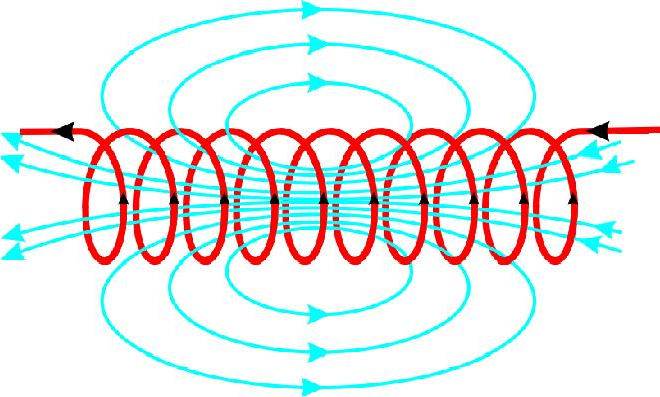
\includegraphics[height=3.8cm]{solenoid_field.png}};
  \node[anchor=north west,text width=9.4cm,font=\sffamily,align=left] at ([xshift=1.8cm,yshift=-10.8cm]current page.north west) {%
    {\large\bfseries Practise the way the exam asks.}\\[6pt]
    \small Every topic of the chapter, turned into questions you answer in this book:
    fill in the blanks, label and draw field lines, apply the hand rules, complete the
    derivation, solve the numerical, explain the reason. Each unit ends with a self check,
    and the book ends with a full 40-mark chapter test.\\[10pt]
    \faStar\ Marks badges: \badge{1M} \badge{2M} \badge{4M}\\[4pt]
    \faStar\ Academic standards: \asbadge{AS1} concept \asbadge{AS3} experiment \asbadge{AS5} diagram \asbadge{AS7} application\\[4pt]
    \faStar\ \tb\ marks every question from \emph{Improve your learning}};
  \node[anchor=south west,font=\sffamily] at ([xshift=1.8cm,yshift=2.2cm]current page.south west) {%
    \renewcommand{\arraystretch}{2.1}
    \begin{tabular}{@{}l@{\quad}p{8.5cm}@{}}
    \textbf{Name} & \hrulefill\\
    \textbf{Class / Section} & \hrulefill\\
    \textbf{Roll No.} & \hrulefill\\
    \textbf{School} & \hrulefill\\
    \end{tabular}};
\end{tikzpicture}
\null\clearpage

% =====================================================================
\section*{\sffamily\color{ecblue}How to use this workbook}
\begin{enumerate}[label=\textcolor{ecorange}{\faArrowRight},leftmargin=6mm]
\item Read the \textbf{Recall in 60 seconds} box first. If a point feels new, go back to the textbook page before you start.
\item Answer in the book, in pen. Do the questions \textbf{without} looking at the textbook, then check.
\item Numericals: \emph{formula $\rightarrow$ values in SI units (m, m$^2$, A, T) $\rightarrow$ answer with unit}.
\item Field-line diagrams: draw in pencil, put \textbf{arrows on every line}, mark N and S, $\odot$ and $\otimes$.
\item For every direction question, write which \textbf{rule} you used (thumb rule, right hand rule, Lenz's law).
\item Fill in the \textbf{Self check} after each unit; copy mistakes into the \textbf{Mistake log}.
\end{enumerate}

\subsection*{\sffamily\color{ecblue}What the exam asks from this chapter}
\renewcommand{\arraystretch}{1.35}
\begin{tabularx}{\linewidth}{>{\bfseries\sffamily}p{1.6cm}X}
\toprule
\rowcolor{ecblue}\textcolor{white}{Marks} & \textcolor{white}{\textbf{\sffamily Typical questions}}\\
\midrule
1 mark & Units (weber, tesla), one-line laws, energy change in motor/generator, force when parallel to $B$, MCQs.\\
2 marks & Direction of current/field/force from a figure, pole of a coil, TV distortion, closed field lines, short numericals on $B=\Phi/A$, $F=ILB$, $\varepsilon=Blv$, $\varepsilon=N\Delta\Phi/\Delta t$.\\
4 marks & Activities: current produces a field; force on a wire; Faraday's law. Working of motor and generators. Derivation of $\varepsilon=Blv$, $F=ILB$, $r=mv/Bq$. Lenz's law with energy argument. Levitation.\\
Diagrams & Field lines of bar magnet, straight wire, solenoid; right hand rules; coil in a field; motor; Faraday's activity; AC generator and emf graph.\\
\bottomrule
\end{tabularx}

\subsection*{\sffamily\color{ecblue}My progress tracker}
\renewcommand{\arraystretch}{1.55}
\begin{tabularx}{\linewidth}{>{\sffamily}l X c c c}
\toprule
\rowcolor{ecteal!15}\textbf{Unit} & \textbf{Topic} & \textbf{Score} & \textbf{Confidence} & \textbf{Revised on}\\
\midrule
1 & Oersted, magnetic field and field lines & \rule{1.3cm}{0.3pt} & \tick\,\tick\,\tick & \rule{1.6cm}{0.3pt}\\
2 & Magnetic flux and flux density & \rule{1.3cm}{0.3pt} & \tick\,\tick\,\tick & \rule{1.6cm}{0.3pt}\\
3 & Fields of a wire, coil and solenoid & \rule{1.3cm}{0.3pt} & \tick\,\tick\,\tick & \rule{1.6cm}{0.3pt}\\
4 & Force on a moving charge & \rule{1.3cm}{0.3pt} & \tick\,\tick\,\tick & \rule{1.6cm}{0.3pt}\\
5 & Force on a current; electric motor & \rule{1.3cm}{0.3pt} & \tick\,\tick\,\tick & \rule{1.6cm}{0.3pt}\\
6 & Induction: Faraday, Lenz, motional emf & \rule{1.3cm}{0.3pt} & \tick\,\tick\,\tick & \rule{1.6cm}{0.3pt}\\
7 & Applications, levitation, generators & \rule{1.3cm}{0.3pt} & \tick\,\tick\,\tick & \rule{1.6cm}{0.3pt}\\
-- & One-mark rapid fire & \rule{1.3cm}{0.3pt} & \tick\,\tick\,\tick & \rule{1.6cm}{0.3pt}\\
-- & Chapter test (40 marks) & \rule{1.3cm}{0.3pt} & \tick\,\tick\,\tick & \rule{1.6cm}{0.3pt}\\
\bottomrule
\end{tabularx}
{\small Confidence: tick one box for ``shaky'', two for ``fine'', three for ``I can teach it''.}

% =====================================================================
\unit{Magnetic field and field lines}{\badge{1M}\ \badge{2M}\ \badge{4M}}
% =====================================================================
\begin{recall}
\begin{itemize}[leftmargin=5mm,itemsep=0pt]
\item \key{Oersted (1820)}: a compass needle under a wire deflects when current flows $\Rightarrow$ a current produces a magnetic field.
\item A \key{magnetic field} is the region around a magnet where its force acts without contact. It has \textbf{strength} and \textbf{direction} and is three-dimensional.
\item \key{Field lines} are imaginary; the \textbf{tangent} gives the direction; crowded lines = strong field. Outside a magnet they go N $\to$ S. Uniform field: parallel, equally spaced lines.
\end{itemize}
\end{recall}

\exhead{A}{Fill in the blanks}{\asbadge{AS1}\ \badge{1M}}
\begin{enumerate}
\item The scientist who first showed that a current deflects a compass needle was \blank{Oersted}.
\item The direction of the field at a point is given by the \blank{tangent} to the field line at that point.
\item Field lines are \blank{crowded} near the poles, where the field is \blank{strong}.
\item A field whose strength and direction are the same everywhere is called a \blank{uniform} field.
\item Outside a bar magnet field lines go from \blank[1.5cm]{N} to \blank[1.5cm]{S}.
\end{enumerate}

\exhead{B}{True or false}{\asbadge{AS1}\ \badge{1M}}
{\small Write T or F. If false, correct it on the line below.}
\begin{enumerate}
\tf{Field lines of a magnet can cross each other.}{F}{They never cross; at a crossing the field would have two directions, which is impossible.}
\ifanswers\else\writelines{1}\fi
\tf{The magnetic field of a bar magnet exists only in the plane of the paper.}{F}{It is three-dimensional; it surrounds the magnet in all directions.}
\ifanswers\else\writelines{1}\fi
\tf{Far from a magnet a compass needle points almost north--south.}{T}{}
\ifanswers\else\writelines{1}\fi
\end{enumerate}

\exhead{C}{Label the Oersted apparatus}{\asbadge{AS5}\ \badge{2M}}
\begin{center}
\figlab{oersted_setup.png}{width=0.62\linewidth}{
\draw[fptr] (0.18,1.12) node[flab,anchor=south]{(a) \blank[2.3cm]{copper wire}} -- (0.36,0.82);
\draw[fptr] (0.85,1.12) node[flab,anchor=south]{(b) \blank[2.3cm]{battery}} -- (0.66,0.78);
\draw[fptr] (0.20,0.05) node[flab,anchor=north]{(c) \blank[2.3cm]{compass}} -- (0.40,0.60);
\draw[fptr] (0.72,0.05) node[flab,anchor=north]{(d) \blank[2.3cm]{key}} -- (0.54,0.40);}
\end{center}
\vspace{6pt}
\begin{enumerate}
\item What happens to the needle when the key is closed? What does it prove? \mk{2M}
\answer[3]{The needle deflects. When the key is opened it returns to the north--south direction. This proves that a current-carrying wire produces a magnetic field around it: electricity and magnetism are related.}
\end{enumerate}

\exhead{D}{Draw field lines}{\asbadge{AS5}\ \badge{2M}}
Draw at least six field lines of the bar magnet below, with arrows. \mk{2M}
\begin{center}
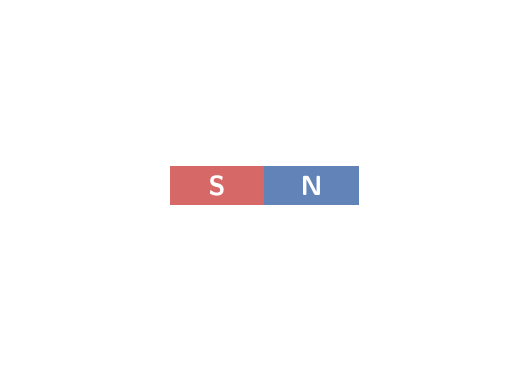
\begin{tikzpicture}
\fill[ecred!70] (-1.2,-0.25) rectangle (0,0.25); \fill[ecblue!70] (0,-0.25) rectangle (1.2,0.25);
\node[white,font=\sffamily\bfseries] at (-0.6,0) {S}; \node[white,font=\sffamily\bfseries] at (0.6,0) {N};
\ifanswers
\foreach \h in {0.8,1.4,2.1}{
  \draw[afl=0.5] (1.2,0.1) .. controls (2.5,\h) and (-2.5,\h) .. (-1.2,0.1);
  \draw[afl=0.5] (1.2,-0.1) .. controls (2.5,-\h) and (-2.5,-\h) .. (-1.2,-0.1);}
\draw[afl=0.5] (1.2,0) -- (3,0); \draw[afl=0.5] (-3,0) -- (-1.2,0);
\else
\draw[white] (-3,-2) rectangle (3,2);
\fi
\end{tikzpicture}
\end{center}

\exhead{E}{Short answers}{\tb\ \asbadge{AS1}\ \badge{2M}}
\begin{enumerate}
\item Are magnetic field lines closed? Explain. \mk{2M}
\answer[4]{Yes. Around a straight wire they are complete circles. For a solenoid (and a bar magnet) the lines outside go from N to S and continue inside from S to N, so every line is a closed loop.}
\item How can you find the strength and the direction of a magnetic field using field lines? \mk{2M}
\answer[3]{Direction: the tangent to the field line at the point (the way a compass needle points). Strength: how close the lines are; crowded lines mean a strong field, widely spaced lines a weak field.}
\end{enumerate}

\selfcheck{19}{
\item describe Oersted's experiment and its conclusion
\item state the properties of field lines
\item draw the field lines of a bar magnet with arrows}

% =====================================================================
\unit{Magnetic flux and flux density}{\badge{1M}\ \badge{2M}}
% =====================================================================
\begin{recall}
\begin{itemize}[leftmargin=5mm,itemsep=0pt]
\item \key{Magnetic flux} $\Phi$: number of field lines through a plane held perpendicular to the field. Unit \imp{weber (Wb)}.
\item \key{Flux density} $B=\dfrac{\Phi}{A}$ (area perpendicular to the field). Unit \imp{Wb/m$^2$ = tesla (T)}.
\item Plane tilted so its normal makes $\theta$ with $B$: effective area $A\cos\theta$, so \imp{$\Phi=BA\cos\theta$}. Plane parallel to $B$: $\Phi=0$.
\end{itemize}
\end{recall}

\exhead{A}{Fill in the blanks}{\asbadge{AS1}\ \badge{1M}}
\begin{enumerate}
\item The SI unit of magnetic flux is the \blank{weber}.
\item The SI unit of magnetic flux density is the \blank{tesla}, which equals \blank{Wb/m$^2$}.
\item Magnetic flux density is also called magnetic \blank{induction}.
\item The flux through a plane held parallel to the field is \blank[1.5cm]{zero}.
\end{enumerate}

\exhead{B}{Complete the derivation of $\Phi=BA\cos\theta$}{\asbadge{AS1}\ \badge{2M}}
\noindent
\begin{minipage}[c]{0.38\linewidth}\centering
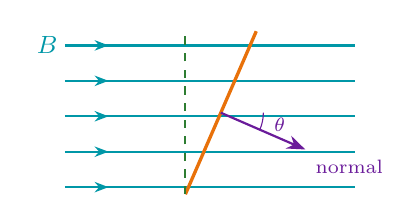
\begin{tikzpicture}[scale=0.9]
\foreach \y in {0.2,0.7,1.2,1.7,2.2} \draw[fl=0.15] (-0.5,\y) -- (3.6,\y);
\node[font=\small\bfseries,fieldc] at (-0.75,2.2) {$B$};
\draw[very thick,ecorange] (1.2,0.1) -- (2.2,2.4);
\coordinate (C) at (1.7,1.25);
\draw[-{Stealth},thick,ecpurple] (C) -- ($(C)+(-23.5:1.3)$) node[below right,font=\scriptsize]{normal};
\draw[ecpurple] ($(C)+(0.6,0)$) arc (0:-23.5:0.6); \node[font=\scriptsize,ecpurple] at ($(C)+(-12:0.85)$) {$\theta$};
\draw[thick,dashed,ecgreen] (1.2,0.1) -- (1.2,2.4);
\end{tikzpicture}\\{\small edge view of a plane of area $A$}
\end{minipage}\hfill
\begin{minipage}[c]{0.58\linewidth}
(1) $B$ uses the area \blank{perpendicular} to the field:\\ \hspace*{6mm}$B=\dfrac{\Phi}{A_\perp}$\\[4pt]
(2) The effective area perpendicular to the field is $A_\perp=\mblank{A\cos\theta}$.\\[4pt]
(3) So $B=\mblank[2.2cm]{\dfrac{\Phi}{A\cos\theta}}$ and $\Phi=\mblank[2.2cm]{BA\cos\theta}$.\\[4pt]
(4) $\theta=0^\circ$: $\Phi=\mblank{BA}$;\quad $\theta=90^\circ$: $\Phi=\mblank{0}$.
\end{minipage}

\exhead{C}{Numericals}{\asbadge{AS7}\ \badge{2M}}
\begin{worked}[Worked example: 0.02 Wb crosses 0.4 m$^2$ normally]
$B=\dfrac{\Phi}{A}=\dfrac{0.02}{0.4}=0.05$ T.\quad \textbf{Always} convert cm$^2$ to m$^2$ (1 cm$^2=10^{-4}$ m$^2$).
\end{worked}
\begin{enumerate}
\item $B=0.8$ T passes normally through a loop of area 0.05 m$^2$. Find the flux. \mk{2M}
\answer[2]{$\Phi=BA=0.8\times0.05=0.04$ Wb.}
\item The same loop is turned so that its normal makes $60^\circ$ with the field. Find the new flux. \mk{2M}
\answer[2]{$\Phi=BA\cos60^\circ=0.04\times\frac12=0.02$ Wb.}
\item A flux of $6\times10^{-4}$ Wb passes normally through 20 cm$^2$. Find $B$. \mk{2M}
\answer[3]{$A=20\times10^{-4}=2\times10^{-3}$ m$^2$. $B=\dfrac{6\times10^{-4}}{2\times10^{-3}}=0.3$ T.}
\end{enumerate}

\selfcheck{15}{
\item define magnetic flux and flux density with units
\item derive $\Phi=BA\cos\theta$ and use its special cases
\item convert areas to m$^2$ in numericals}

% =====================================================================
\unit{Fields of a wire, a coil and a solenoid}{\badge{1M}\ \badge{2M}\ \badge{4M}}
% =====================================================================
\begin{recall}
\begin{itemize}[leftmargin=5mm,itemsep=0pt]
\item \key{Straight wire}: field lines are concentric circles. \textbf{Right hand thumb rule}: thumb along current, curled fingers give the field. Out of the page $\odot$ $\Rightarrow$ anticlockwise; into the page $\otimes$ $\Rightarrow$ clockwise.
\item \key{Circular coil}: field at the centre is perpendicular to the plane of the coil. Curl fingers along the current, thumb gives $B$. Anticlockwise current (as seen) $\Rightarrow$ that face is \textbf{N}.
\item \key{Solenoid}: behaves like a bar magnet; outside N $\to$ S, inside S $\to$ N; lines are closed loops.
\end{itemize}
\end{recall}

\exhead{A}{Draw the field lines}{\asbadge{AS5}\ \badge{2M}}
Draw three field lines with arrows around each wire. \mk{2M}
\begin{center}
\begin{tabular}{c@{\hspace{2cm}}c}
\begin{tikzpicture}
\ifanswers\foreach \r in {0.5,0.9,1.3} \draw[anscol,thick,postaction={decorate},decoration={markings,mark=at position 0.25 with {\arrow{Stealth[length=5pt]}},mark=at position 0.75 with {\arrow{Stealth[length=5pt]}}}] (0,0) circle (\r);
\else\draw[white] (-1.4,-1.4) rectangle (1.4,1.4);\fi
\outpage{(0,0)}
\end{tikzpicture} &
\begin{tikzpicture}
\ifanswers\foreach \r in {0.5,0.9,1.3} \draw[anscol,thick,postaction={decorate},decoration={markings,mark=at position 0.25 with {\arrowreversed{Stealth[length=5pt]}},mark=at position 0.75 with {\arrowreversed{Stealth[length=5pt]}}}] (0,0) circle (\r);
\else\draw[white] (-1.4,-1.4) rectangle (1.4,1.4);\fi
\inpage{(0,0)}
\end{tikzpicture}\\
(1) current out of the page & (2) current into the page\\
\ifanswers{\small\color{anscol}anticlockwise}\fi & \ifanswers{\small\color{anscol}clockwise}\fi\\
\end{tabular}
\end{center}

\exhead{B}{Direction questions from the textbook}{\tb\ \asbadge{AS1}\ \badge{1M}\ \badge{2M}}
\noindent
\begin{minipage}[t]{0.22\linewidth}\centering
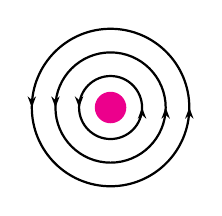
\begin{tikzpicture}[scale=0.5]
\foreach \r in {0.8,1.4,2.0} \draw[thick,postaction={decorate},decoration={markings,mark=at position 0.0 with {\arrow{Stealth[length=4pt]}},mark=at position 0.5 with {\arrow{Stealth[length=4pt]}}}] (0,0) circle (\r);
\fill[magenta] (0,0) circle (0.4);
\end{tikzpicture}\\{\small fig-Q1}
\end{minipage}\hfill
\begin{minipage}[t]{0.75\linewidth}
\begin{enumerate}
\item Field lines around a wire are shown in fig-Q1 (anticlockwise). What is the direction of the current? \mk{1M}
\answer[2]{Out of the page (towards the reader), by the right hand thumb rule.}
\end{enumerate}
\end{minipage}\\[6pt]
\begin{minipage}[t]{0.22\linewidth}\centering
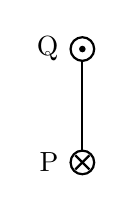
\begin{tikzpicture}[scale=0.6]
\draw[thick] (0,-1) -- (0,1);
\outpage[0.25]{(0,1.2)} \node[left] at (-0.3,1.2) {Q};
\inpage[0.25]{(0,-1.2)} \node[left] at (-0.3,-1.2) {P};
\end{tikzpicture}\\{\small fig-Q3}
\end{minipage}\hfill
\begin{minipage}[t]{0.75\linewidth}
\begin{enumerate}[start=2]
\item A coil is kept perpendicular to the page. At P the current flows into the page, at Q it comes out (fig-Q3). What is the direction of the field due to the coil? \mk{2M}
\answer[3]{At the centre, the wire at P (into page, clockwise field) gives a field to the right; the wire at Q (out of page, anticlockwise field) also gives a field to the right. So the field is along the axis of the coil, from left to right, perpendicular to the plane of the coil.}
\end{enumerate}
\end{minipage}\\[6pt]
\begin{minipage}[t]{0.22\linewidth}\centering
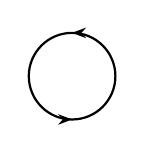
\begin{tikzpicture}[scale=0.55]
\draw[thick,postaction={decorate},decoration={markings,mark=at position 0.25 with {\arrow{Stealth[length=5pt]}},mark=at position 0.75 with {\arrow{Stealth[length=5pt]}}}] (0,0) circle (1);
\end{tikzpicture}\\{\small fig-Q4}
\end{minipage}\hfill
\begin{minipage}[t]{0.75\linewidth}
\begin{enumerate}[start=3]
\item The current in a coil flows as in fig-Q4 (anticlockwise as you see it). What pole is formed at this face? \mk{1M}
\answer[2]{North pole: curling the right-hand fingers anticlockwise, the thumb (field) points towards the viewer.}
\end{enumerate}
\end{minipage}

\exhead{C}{Label the solenoid}{\asbadge{AS5}\ \badge{2M}}
In the figure the current enters at the right end and leaves at the left. Mark the N and S ends and the direction of the field inside.
\begin{center}
\figlab{solenoid_field.png}{width=0.55\linewidth}{
\node[font=\sffamily\bfseries] at (-0.06,0.5) {\ifanswers\textcolor{anscol}{N}\else\fbox{\phantom{N}}\fi};
\node[font=\sffamily\bfseries] at (1.06,0.5) {\ifanswers\textcolor{anscol}{S}\else\fbox{\phantom{S}}\fi};
\ifanswers\draw[-{Stealth[length=6pt]},anscol,very thick] (0.75,0.5) -- (0.25,0.5) node[midway,below=6pt,font=\small]{inside: S $\to$ N};\fi}
\end{center}

\exhead{D}{Experiment}{\tb\ \asbadge{AS3}\ \badge{4M}}
Explain with the help of two activities that a current-carrying wire produces a magnetic field. \mk{4M}
\answer[12]{\textbf{Activity 1 (Oersted):} a wire stretched through the slits of two sticks is connected to a battery through a key; a compass is placed below it. When the key is closed the needle deflects; when it is opened the needle returns to N--S.\\
\textbf{Activity 4:} a vertical wire passes through a hole in a plank; 6--10 compass needles are placed on a circle around it. When the current flows, the needles set along tangents to the circle; iron filings sprinkled around form concentric circles.\\
\textbf{Conclusion:} the wire produces a magnetic field whose lines are concentric circles around it; the direction is given by the right hand thumb rule.}

\selfcheck{20}{
\item draw the field of a straight wire for both current directions
\item find the pole of a coil face from the current direction
\item describe the field of a solenoid and why its lines are closed loops}

% =====================================================================
\unit{Force on a moving charge}{\badge{1M}\ \badge{2M}\ \badge{4M}}
% =====================================================================
\begin{recall}
\begin{itemize}[leftmargin=5mm,itemsep=0pt]
\item A magnet distorts the picture on a CRT TV: the field exerts a force on the moving electrons.
\item \imp{$F=qvB\sin\theta$}; $F=qvB$ when $v\perp B$; $F=0$ when $v\parallel B$ or $v=0$.
\item Direction: right hand rule (forefinger $v$, middle finger $B$, thumb $F$), for a \textbf{positive} charge; reverse it for an electron. $F$ is always perpendicular to both $v$ and $B$.
\item A charge moving $\perp B$ goes round a circle: $r=\dfrac{mv}{Bq}$, $T=\dfrac{2\pi m}{Bq}$.
\end{itemize}
\end{recall}

\exhead{A}{Fill in the blanks}{\asbadge{AS1}\ \badge{1M}}
\begin{enumerate}
\item The force on a charge moving parallel to the field is \blank[1.5cm]{zero}.
\item The magnetic force is always perpendicular to both the \blank{velocity} and the \blank{field}.
\item For an electron, the direction of force is \blank{opposite} to that found for a positive charge.
\item The magnetic force on a charge moving $\perp B$ acts as the \blank{centripetal} force.
\end{enumerate}

\exhead{B}{Complete the derivation}{\asbadge{AS1}\ \badge{4M}}
A charge $q$ of mass $m$ moves with speed $v$ perpendicular to a uniform field $B$.\\[4pt]
(1) Magnetic force: $F=\mblank{qvB}$ \quad(since $\sin90^\circ=\mblank[1cm]{1}$).\\[4pt]
(2) This force is always perpendicular to the velocity, so the path is a \blank{circle}.\\[4pt]
(3) Centripetal force = magnetic force: \quad $\mblank{\dfrac{mv^2}{r}}=qvB$ \quad$\Rightarrow$\quad $r=\mblank[2cm]{\dfrac{mv}{Bq}}$\\[4pt]
(4) Time period $T=\dfrac{2\pi r}{v}=\mblank[2.2cm]{\dfrac{2\pi m}{Bq}}$, which does \blank{not} depend on the speed.

\exhead{C}{Numericals}{\asbadge{AS7}\ \badge{2M}}
\begin{enumerate}
\item A charge of $2\times10^{-6}$ C moves at $3\times10^4$ m/s perpendicular to $B=0.5$ T. Find the force. \mk{2M}
\answer[2]{$F=qvB=2\times10^{-6}\times3\times10^4\times0.5=3\times10^{-2}$ N.}
\item The same charge moves at $30^\circ$ to the field. Find the force. \mk{2M}
\answer[2]{$F=qvB\sin30^\circ=0.03\times\frac12=1.5\times10^{-2}$ N.}
\item A proton ($m=1.67\times10^{-27}$ kg, $q=1.6\times10^{-19}$ C) moves at $10^6$ m/s perpendicular to $B=1$ T. Find the radius of its path. \mk{2M}
\answer[3]{$r=\dfrac{mv}{Bq}=\dfrac{1.67\times10^{-27}\times10^6}{1\times1.6\times10^{-19}}=1.04\times10^{-2}$ m $\approx1$ cm.}
\end{enumerate}

\exhead{D}{Short answers}{\tb\ \asbadge{AS1}\ \badge{2M}}
\begin{enumerate}
\item Why does the picture appear distorted when a bar magnet is brought close to the screen of a television? \mk{2M}
\answer[3]{The picture on a CRT screen is made by a beam of fast-moving electrons. The magnet's field exerts a force $F=qvB\sin\theta$ on them, which changes their path, so they strike the wrong spots and the picture is distorted.}
\item State the right hand rule for the direction of force on a positive charge. \mk{2M}
\answer[3]{Stretch the thumb, forefinger and middle finger of the right hand mutually perpendicular. If the forefinger points along the velocity (or current) and the middle finger along the field, the thumb gives the direction of the force.}
\end{enumerate}

\selfcheck{25}{
\item use $F=qvB\sin\theta$ including the zero-force cases
\item find the direction of force with the right hand rule, and reverse it for electrons
\item derive $r=mv/Bq$ and $T=2\pi m/Bq$}

% =====================================================================
\unit{Force on a current; electric motor}{\badge{1M}\ \badge{2M}\ \badge{4M}}
% =====================================================================
\begin{recall}
\begin{itemize}[leftmargin=5mm,itemsep=0pt]
\item A current is moving charge, so a current-carrying wire in a field feels a force: \imp{$F=ILB\sin\theta$}; $F=ILB$ when $I\perp B$; $F=0$ when $I\parallel B$.
\item Activity 8: a wire in a horseshoe magnet is deflected; reversing the current or the poles reverses the deflection.
\item \key{Motor}: forces on opposite sides of a coil are equal and opposite (net force 0) but form a \textbf{couple} that rotates the coil. \textbf{Split rings} and brushes reverse the current every half turn. Electrical $\to$ mechanical energy.
\end{itemize}
\end{recall}

\exhead{A}{Complete the derivation of $F=ILB$}{\asbadge{AS1}\ \badge{4M}}
(1) Force on one charge moving with drift velocity $v$ perpendicular to $B$: $F_0=\mblank{qvB}$.\\[4pt]
(2) Total charge in the length $L$ inside the field is $Q$: $F=\mblank{QvB}$ \dots(1)\\[4pt]
(3) Time to cross length $L$: $t=\dfrac{L}{v}$, so $v=\mblank{\dfrac{L}{t}}$ \dots(2)\\[4pt]
(4) Put (2) in (1): $F=\mblank[2.2cm]{\dfrac{Q}{t}LB}$ \dots(3)\\[4pt]
(5) Since $\dfrac{Q}{t}=\mblank[1cm]{I}$, \quad $F=\mblank[1.6cm]{ILB}$. At an angle $\theta$: $F=\mblank[2cm]{ILB\sin\theta}$.

\exhead{B}{Numericals}{\tb\ \asbadge{AS7}\ \badge{2M}}
\begin{enumerate}
\item \tb\ An 8 N force acts on a 20 cm conductor placed perpendicular to a magnetic field. The current is 40 A. Find the magnetic field induction. \mk{2M}
\answer[3]{$L=0.2$ m. $B=\dfrac{F}{IL}=\dfrac{8}{40\times0.2}=1$ T.}
\item A wire 0.5 m long carries 4 A at $30^\circ$ to a field of 0.2 T. Find the force. \mk{2M}
\answer[2]{$F=ILB\sin30^\circ=4\times0.5\times0.2\times\frac12=0.2$ N.}
\end{enumerate}

\exhead{C}{Direction of force}{\tb\ \asbadge{AS1}\ \badge{2M}}
\noindent
\begin{minipage}[c]{0.3\linewidth}\centering
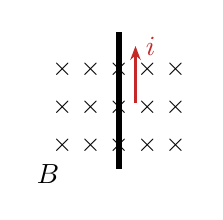
\begin{tikzpicture}[scale=0.6]
\foreach \x in {-2,...,2}{\foreach \y in {-1,...,1}{\node[font=\small] at (\x*0.6,\y*0.8) {$\times$};}}
\draw[line width=2pt] (0,-1.3) -- (0,1.6);
\draw[cur] (0.35,0.1) -- (0.35,1.3) node[right]{$i$};
\node at (-1.5,-1.4) {$B$};
\end{tikzpicture}\\{\small fig-Q5}
\end{minipage}\hfill
\begin{minipage}[c]{0.67\linewidth}
A straight wire carrying current $i$ upward is kept perpendicular to a field directed into the page; length $L$ is in the field. Find the magnitude and direction of the force. \mk{2M}
\answer[3]{Magnitude $F=iLB$ (since $\theta=90^\circ$). Right hand rule: forefinger up ($i$), middle finger into the page ($B$) $\Rightarrow$ thumb points to the \textbf{left}. The force acts to the left, in the plane of the page.}
\end{minipage}

\exhead{D}{Motor}{\asbadge{AS1}\ \asbadge{AS5}\ \badge{4M}}
\noindent
\begin{minipage}[c]{0.38\linewidth}\centering
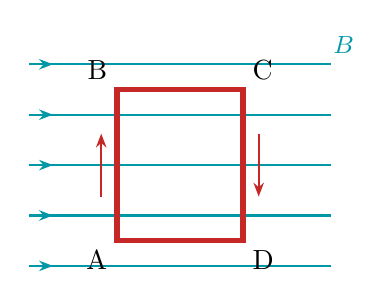
\begin{tikzpicture}[scale=0.8]
\foreach \y in {-1.6,-0.8,0,0.8,1.6} \draw[fl=0.08] (-2.4,\y) -- (2.4,\y);
\node[font=\small\bfseries,fieldc] at (2.6,1.9) {$B$};
\draw[ecred,line width=2pt] (-1,-1.2) -- (-1,1.2) -- (1,1.2) -- (1,-1.2) -- cycle;
\draw[cur] (-1.25,-0.5) -- (-1.25,0.5); \draw[cur] (1.25,0.5) -- (1.25,-0.5);
\node[below left] at (-1,-1.2) {A}; \node[above left] at (-1,1.2) {B};
\node[above right] at (1,1.2) {C}; \node[below right] at (1,-1.2) {D};
\end{tikzpicture}
\end{minipage}\hfill
\begin{minipage}[c]{0.6\linewidth}
\begin{enumerate}
\item The force on AB is directed \blank{into the page} and on CD \blank{out of the page}.\mk{1M}
\item The net force on the coil is \blank[1.5cm]{zero}, yet the coil \blank{rotates} because the two forces form a \blank{couple}. \mk{1M}
\item Why is the current reversed every half turn, and which part does it? \mk{2M}
\answer[3]{After half a turn the forces would turn the coil back, so it would only rock to and fro. The split rings (commutator), rotating with the coil, swap brushes every half turn, reversing the current so the rotation continues in the same direction.}
\end{enumerate}
\end{minipage}

\exhead{E}{Experiment}{\tb\ \asbadge{AS3}\ \badge{4M}}
How do you verify experimentally that a current-carrying conductor experiences a force when kept in a magnetic field? \mk{4M}
\answer[10]{\textbf{Materials:} wooden plank, two split sticks, copper wire, 9 V battery, switch, horseshoe magnet.\\
\textbf{Procedure:} pass the wire through the splits of the sticks and connect it to the battery through the switch. Close the switch and bring the horseshoe magnet so the wire lies between its poles.\\
\textbf{Observation:} the wire is deflected (pushed up or down). Reversing the poles of the magnet, or the direction of the current, reverses the deflection.\\
\textbf{Conclusion:} a current-carrying conductor in a field experiences a force $F=ILB$; its direction is given by the right hand rule.}

\selfcheck{27}{
\item derive $F=ILB$ from $F=qvB$
\item find the direction of force on a wire with the right hand rule
\item explain the working of a motor, including split rings}

% =====================================================================
\unit{Induction: Faraday, Lenz and motional emf}{\badge{1M}\ \badge{2M}\ \badge{4M}}
% =====================================================================
\begin{recall}
\begin{itemize}[leftmargin=5mm,itemsep=0pt]
\item \key{Electromagnetic induction}: a current is induced in a coil when the flux through it changes (relative motion of magnet and coil).
\item \key{Faraday's law}: $\varepsilon=\dfrac{\Delta\Phi}{\Delta t}$; for $N$ turns $\varepsilon=N\dfrac{\Delta\Phi_0}{\Delta t}$.
\item \key{Lenz's law}: the induced current opposes the change in flux (conservation of energy). N pole approaching $\Rightarrow$ near face of coil becomes N.
\item \key{Motional emf}: $\varepsilon=Blv$ for a conductor of length $l$ moving with speed $v$ perpendicular to $B$.
\end{itemize}
\end{recall}

\exhead{A}{Activity 9: what does the galvanometer show?}{\asbadge{AS3}\ \badge{1M}}
\renewcommand{\arraystretch}{1.7}
\begin{tabularx}{\linewidth}{>{\small}X>{\small}X}
\toprule
\rowcolor{ecblue}\textcolor{white}{\textbf{Action}} & \textcolor{white}{\textbf{Galvanometer}}\\
\midrule
Magnet held at rest inside the coil & \blank{no deflection}\\
N pole pushed towards the coil & \blank{deflects one way}\\
N pole pulled away from the coil & \blank{deflects the opposite way}\\
S pole pushed towards the coil & \blank{deflects opposite to N pushed in}\\
Magnet pushed in faster & \blank{larger deflection}\\
\bottomrule
\end{tabularx}

\exhead{B}{Fill in the blanks}{\asbadge{AS1}\ \badge{1M}}
\begin{enumerate}
\item The current produced by changing flux is called the \blank{induced current}.
\item Lenz's law is a consequence of the conservation of \blank{energy}.
\item When the N pole of a magnet approaches a coil, the face of the coil nearer to it becomes a \blank[1.5cm]{north} pole.
\item $\varepsilon=Blv$ is called the \blank{motional emf}.
\end{enumerate}

\exhead{C}{Complete the derivation of $\varepsilon=Blv$}{\asbadge{AS1}\ \badge{4M}}
A cross wire of length $l$ lies on two parallel conductors in a uniform field $B$. It is moved a distance $s$ in time $\Delta t$ and a current $I$ flows.\\[4pt]
(1) Force of the field on the cross wire: $F=\mblank{BIl}$ \dots(8)\\[4pt]
(2) Work done by us in moving it: $W=Fs=\mblank{BIls}$ \dots(9)\\[4pt]
(3) Change in flux as the loop area changes by $ls$: $\Delta\Phi=\mblank{Bls}$ \dots(10) \;$\Rightarrow W=\mblank{I\,\Delta\Phi}$\\[4pt]
(4) Dividing by $\Delta t$: $P=\dfrac{W}{\Delta t}=\mblank{\dfrac{I\Delta\Phi}{\Delta t}}$; comparing with $P=\varepsilon I$ gives $\varepsilon=\mblank{\dfrac{\Delta\Phi}{\Delta t}}$\\[4pt]
(5) Also $P=Fv=\mblank{BIlv}$ (since $\dfrac{s}{\Delta t}=v$). So $\varepsilon I=BIlv$ \;$\Rightarrow\;\varepsilon=\mblank[1.6cm]{Blv}$

\exhead{D}{Numericals}{\tb\ \asbadge{AS7}\ \badge{2M}}
\begin{worked}[Worked example (textbook): 400 turns, flux per turn rises by 0.001 Wb in 0.1 s]
$\varepsilon=N\dfrac{\Delta\Phi_0}{\Delta t}=\dfrac{400\times0.001}{0.1}=4$ V. While the flux stays constant (0.1 s to 0.3 s), $\varepsilon=0$.
\end{worked}
\begin{enumerate}
\item \tb\ Find the length of a conductor moving at 10 m/s perpendicular to a field of 0.8 T if it induces an emf of 8 V. \mk{2M}
\answer[2]{$l=\dfrac{\varepsilon}{Bv}=\dfrac{8}{0.8\times10}=1$ m.}
\item The flux per turn in a coil of 100 turns falls from 0.05 Wb to 0.01 Wb in 0.2 s. Find the induced emf. \mk{2M}
\answer[3]{$\Delta\Phi_0=0.04$ Wb. $\varepsilon=\dfrac{100\times0.04}{0.2}=20$ V.}
\item A 1.5 m rod moves at 2 m/s perpendicular to $B=0.4$ T. Find the emf. \mk{2M}
\answer[2]{$\varepsilon=Blv=0.4\times1.5\times2=1.2$ V.}
\end{enumerate}

\exhead{E}{Figure questions}{\tb\ \asbadge{AS1}\ \asbadge{AS2}\ \badge{2M}}
\noindent
\begin{minipage}[c]{0.3\linewidth}\centering
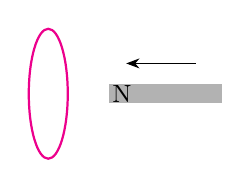
\begin{tikzpicture}[scale=0.55]
\draw[magenta,thick] (0,0) ellipse (0.45 and 1.5);
\fill[gray!60] (1.4,-0.22) rectangle (4,0.22); \node[font=\small] at (1.7,0) {N};
\draw[-{Stealth}] (3.4,0.7) -- (1.8,0.7);
\end{tikzpicture}\\{\small fig-Q2}
\end{minipage}\hfill
\begin{minipage}[c]{0.67\linewidth}
\begin{enumerate}
\item A bar magnet with its N pole facing a coil moves towards it (fig-Q2). What happens to the flux through the coil? Which way does the induced current flow as seen from the magnet? \mk{2M}
\answer[3]{The flux through the coil increases. By Lenz's law the near face becomes N to repel the magnet, so the induced current is anticlockwise as seen from the magnet.}
\end{enumerate}
\end{minipage}\\[6pt]
\begin{minipage}[c]{0.3\linewidth}\centering
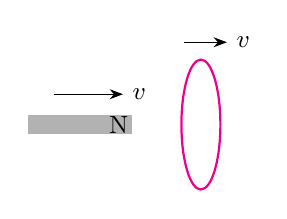
\begin{tikzpicture}[scale=0.55]
\fill[gray!60] (-3,-0.22) rectangle (-0.6,0.22); \node[font=\small] at (-0.9,0) {N};
\draw[-{Stealth}] (-2.4,0.7) -- (-0.8,0.7) node[right,font=\small]{$v$};
\draw[magenta,thick] (1,0) ellipse (0.45 and 1.5);
\draw[-{Stealth}] (0.6,1.9) -- (1.6,1.9) node[right,font=\small]{$v$};
\end{tikzpicture}\\{\small fig-Q6}
\end{minipage}\hfill
\begin{minipage}[c]{0.67\linewidth}
\begin{enumerate}[start=2]
\item \tb\ The coil and the bar magnet both move in the same direction with the same speed (fig-Q6). What happens? \mk{2M}
\answer[3]{There is no relative motion between the magnet and the coil, so the flux through the coil does not change. No emf is induced and no current flows.}
\end{enumerate}
\end{minipage}

\exhead{F}{Long answers}{\tb\ \asbadge{AS1}\ \asbadge{AS3}\ \badge{4M}}
\begin{enumerate}
\item Explain Faraday's law of induction with the help of an activity. \mk{4M}
\answer[10]{\textbf{Activity:} connect a coil to a galvanometer. Push the N pole of a bar magnet into the coil: the needle deflects. Hold it still: no deflection. Pull it out: the needle deflects the other way. With the S pole the deflections reverse. Moving the coil instead of the magnet gives the same result; faster motion gives a larger deflection.\\
\textbf{Law:} whenever the magnetic flux linked with a closed coil changes, an emf (and current) is induced. The induced emf equals the rate of change of flux: $\varepsilon=\dfrac{\Delta\Phi}{\Delta t}$; for $N$ turns, $\varepsilon=N\dfrac{\Delta\Phi_0}{\Delta t}$.}
\item State Lenz's law and show that it follows from the conservation of energy. \mk{4M}
\answer[9]{\textbf{Law:} the induced current flows in a direction that opposes the change in flux producing it.\\
\textbf{Energy argument:} push the N pole towards a coil. If the induced current made the near face S, it would attract the magnet, which would speed up by itself while electrical energy was also produced: energy from nothing, which is impossible. So the near face must be N and repel the magnet; we must do work to push it, and this work becomes electrical energy. Pulling the magnet away, the near face becomes S and attracts it, again opposing the motion.}
\item What experiment do you suggest to understand Faraday's law? What instruments are required? Give suggestions for good results and precautions. \mk{4M}
\answer[9]{\textbf{Experiment:} Activity 9 (magnet moved in and out of a coil connected to a galvanometer).\\
\textbf{Instruments:} coil of many turns of insulated copper wire, strong bar magnet, sensitive galvanometer, connecting wires.\\
\textbf{For good results:} use more turns, a stronger magnet and faster motion.\\
\textbf{Precautions:} tight connections; keep the galvanometer away from the magnet; check the zero before starting; move the magnet along the axis of the coil; do not drop the magnet.}
\end{enumerate}

\selfcheck{44}{
\item describe Activity 9 and state Faraday's law
\item state Lenz's law and give the energy argument
\item derive $\varepsilon=\Delta\Phi/\Delta t$ and $\varepsilon=Blv$
\item solve induced-emf numericals with $N$ turns}

% =====================================================================
\unit{Applications, levitation and generators}{\badge{1M}\ \badge{2M}\ \badge{4M}}
% =====================================================================
\begin{recall}
\begin{itemize}[leftmargin=5mm,itemsep=0pt]
\item Applications of induction: security metal detectors, tape recorder heads, induction stoves, ATM card readers.
\item \key{Levitation}: AC in a coil around an iron core $\Rightarrow$ changing flux through a metal ring $\Rightarrow$ induced current opposes it $\Rightarrow$ repulsion balances the ring's weight. With DC the ring only jumps at switch on/off.
\item \key{AC generator}: coil rotated in a field; full \textbf{slip rings}; emf zero when the coil is vertical, maximum when horizontal; reverses every half turn. \key{DC generator}: half (split) rings keep the output in one direction. Mechanical $\to$ electrical energy.
\end{itemize}
\end{recall}

\exhead{A}{Match the following}{\asbadge{AS1}\ \badge{1M}}
\renewcommand{\arraystretch}{1.3}
\begin{tabularx}{\linewidth}{@{}l l c X@{}}
\toprule
& \textbf{Column A} & & \textbf{Column B}\\
\midrule
1. & Induction stove & \bx{c} & a) Induced current in a large coil triggers an alarm\\
2. & Security check & \bx{a} & b) Magnetised tape moves past a small coil\\
3. & Tape recorder & \bx{b} & c) Induced current heats a metal pan\\
4. & Electric motor & \bx{e} & d) Mechanical energy into electrical energy\\
5. & Generator & \bx{d} & e) Electrical energy into mechanical energy\\
\bottomrule
\end{tabularx}

\exhead{B}{Levitation}{\asbadge{AS1}\ \asbadge{AS7}\ \badge{2M}\ \badge{4M}}
\begin{enumerate}
\item Why does the metal ring levitate when AC is used? \mk{4M}
\answer[8]{The ring is at rest, so the net force on it is zero: an upward force balances its weight. AC changes in size and direction continuously, so the flux through the ring keeps changing and a current is induced in it (Faraday). By Lenz's law this current opposes the change, so the ring's lower face always has the same polarity as the coil's upper face (e.g.\ coil top S, ring bottom S). The repulsion provides the upward force that holds the ring up.}
\item What happens if DC is used instead of AC? Why? \mk{2M}
\answer[3]{The ring jumps up only when the switch is closed (and again when it is opened) and then falls back, because the flux through the ring changes only at those instants. With a steady current there is no change of flux, no induced current and no repulsion.}
\end{enumerate}

\exhead{C}{AC generator}{\asbadge{AS1}\ \asbadge{AS5}\ \badge{2M}\ \badge{4M}}
\begin{enumerate}
\item Sketch the emf produced by an AC generator over one rotation, starting with the coil vertical. Mark where the emf is zero and maximum. \mk{2M}
\drawbox{4.5cm}{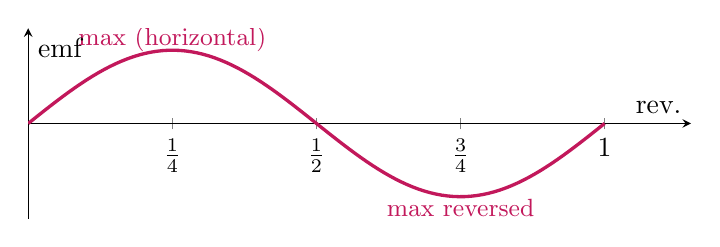
\begin{tikzpicture}
\begin{axis}[width=10cm,height=4cm,axis lines=middle,xmin=0,xmax=1.15,ymin=-1.3,ymax=1.3,
  xtick={0.25,0.5,0.75,1},xticklabels={$\frac14$,$\frac12$,$\frac34$,1},ytick=\empty,xlabel={rev.},ylabel={emf}]
\addplot[anscol,very thick,domain=0:1,samples=100] {sin(deg(2*pi*x))};
\node[font=\small,anscol] at (axis cs:0.25,1.15) {max (horizontal)};
\node[font=\small,anscol] at (axis cs:0.75,-1.15) {max reversed};
\end{axis}\end{tikzpicture}\\\small Zero at 0, $\frac12$, 1 rotation (coil vertical); maximum at $\frac14$ and $\frac34$ (coil horizontal).}
\item Why does the emf vary from zero to maximum during a rotation? \mk{2M}
\answer[3]{The emf depends on how fast the flux through the coil changes. When the coil is vertical (plane $\perp$ field) the flux is maximum but changing slowest, so the emf is zero. When it is horizontal (plane $\parallel$ field) the flux is changing fastest, so the emf is maximum.}
\item How is an AC generator converted into a DC generator? \mk{2M}
\answer[3]{Replace the two full slip rings by two half (split) rings. After every half rotation the ends of the coil change brushes, so the current in the external circuit always flows in the same direction (DC).}
\end{enumerate}

\exhead{D}{Textbook application}{\tb\ \asbadge{AS7}\ \badge{2M}}
Give a few applications of Faraday's law of induction in daily life. \mk{2M}
\answer[4]{Electric generators in power stations; metal detectors at security checks; tape recorder heads; induction stoves; ATM/credit card readers; transformers; bicycle dynamo.}

\selfcheck{25}{
\item explain four applications of induction
\item explain levitation with AC and why DC fails
\item explain the AC generator, its emf graph and the DC version}

% =====================================================================
\clearpage
\section*{\sffamily\color{ecblue}One-mark rapid fire}
{\small Answer in one word or one line. Target \textbf{8 minutes} for 25 questions.}\hfill Time taken: \rule{1.6cm}{0.3pt}\qquad Score: \rule{1cm}{0.3pt} / 25
\vspace{4pt}
\renewcommand{\arraystretch}{1.55}
\begin{multicols}{2}
\begin{enumerate}[itemsep=5pt]
\item Discovered the magnetic effect of current? \blank[2cm]{Oersted}
\item Unit of magnetic flux? \blank[2cm]{weber}
\item Unit of flux density? \blank[2cm]{tesla}
\item 1 T in N, A, m? \blank[2cm]{N/(A m)}
\item $\Phi$ for a plane $\parallel B$? \blank[2cm]{zero}
\item Field lines of a straight wire? \blank[2cm]{circles}
\item Current $\odot$: field lines are? \blank[2cm]{anticlockwise}
\item Rule for field of a wire? \blank[2cm]{thumb rule}
\item Anticlockwise current face is? \blank[2cm]{N pole}
\item Coil that acts like a bar magnet? \blank[2cm]{solenoid}
\item Force on a charge moving $\parallel B$? \blank[2cm]{zero}
\item Formula for force on a charge? \blank[2cm]{$qvB\sin\theta$}
\item Radius of path of a charge? \blank[2cm]{$mv/Bq$}
\item Force on a current $\perp B$? \blank[2cm]{$ILB$}
\item Motor converts? \blank[2cm]{elec.\ $\to$ mech.}
\item Reverses current in a motor? \blank[2cm]{split rings}
\item Faraday's law formula? \blank[2cm]{$\Delta\Phi/\Delta t$}
\item Law giving induced current direction? \blank[2cm]{Lenz's law}
\item Lenz's law is based on? \blank[2cm]{energy cons.}
\item Motional emf? \blank[2cm]{$Blv$}
\item Emf when coil plane $\perp B$ (generator)? \blank[2cm]{zero}
\item Rings in an AC generator? \blank[2cm]{slip rings}
\item Generator converts? \blank[2cm]{mech.\ $\to$ elec.}
\item Stove using induction? \blank[2cm]{induction stove}
\item Current reversing periodically? \blank[2cm]{AC}
\end{enumerate}
\end{multicols}

% =====================================================================
\clearpage
\section*{\sffamily\color{ecblue}Score boosters}
\subsection*{\sffamily Anatomy of a full-marks 4-mark answer}
{\small Example question: \emph{Explain the working of an electric motor.}}\par\vspace{2pt}
\renewcommand{\arraystretch}{1.5}
\begin{tabularx}{\linewidth}{>{\bfseries\sffamily\small}p{2.6cm}X>{\small}p{2.7cm}}
\toprule
\rowcolor{ecteal!15}Part & \textbf{What to write} & \textbf{Why it matters}\\
\midrule
1. Principle & A current-carrying coil in a field experiences a force ($F=ILB$). & Scores the concept mark.\\
2. Diagram & Coil ABCD between N and S, split rings, brushes, battery; arrows for current. & Diagrams carry marks.\\
3. Forces & AB and CD: equal, opposite forces $\Rightarrow$ couple $\Rightarrow$ rotation. & Shows you know why.\\
4. Commutator & Split rings reverse current every half turn $\Rightarrow$ continuous rotation. & Key idea examiners look for.\\
5. Energy & Electrical energy $\to$ mechanical energy. & Closes the answer.\\
\bottomrule
\end{tabularx}

\subsection*{\sffamily Keywords the examiner looks for}
\renewcommand{\arraystretch}{1.35}
\begin{tabularx}{\linewidth}{>{\bfseries\small}p{3.8cm}>{\small}X}
\toprule
Oersted & compass deflects $\cdot$ current produces field\\
Field lines & tangent gives direction $\cdot$ crowded = strong $\cdot$ closed loops\\
Straight wire & concentric circles $\cdot$ right hand thumb rule\\
Force & $qvB\sin\theta$ $\cdot$ $ILB\sin\theta$ $\cdot$ zero when parallel $\cdot$ right hand rule\\
Motor & couple $\cdot$ split rings $\cdot$ brushes $\cdot$ electrical to mechanical\\
Faraday & change of flux $\cdot$ rate of change $\cdot$ induced emf\\
Lenz & opposes the change $\cdot$ conservation of energy\\
Generator & rotating coil $\cdot$ slip rings $\cdot$ zero/maximum emf $\cdot$ mechanical to electrical\\
\bottomrule
\end{tabularx}

\begin{examtip}[Mistakes that cost marks]
\begin{multicols}{2}\small
\begin{itemize}[leftmargin=4mm,itemsep=1pt]
\item Field lines without arrows.
\item $\theta$ measured from the plane, not the normal, in $\Phi=BA\cos\theta$.
\item Forgetting $F=0$ when parallel to $B$.
\item Not reversing the force for an electron.
\item Using cm or cm$^2$ without converting.
\item Forgetting $N$ in $\varepsilon=N\Delta\Phi_0/\Delta t$.
\item Slip rings in a motor (it has split rings).
\item No energy argument in Lenz's law.
\end{itemize}
\end{multicols}
\end{examtip}

\subsection*{\sffamily Formula sheet \normalfont\small(cover the right column and test yourself)}
\renewcommand{\arraystretch}{1.7}
\begin{tabularx}{\linewidth}{>{\bfseries\small}p{5.3cm}X}
\toprule
\rowcolor{ecred}\textcolor{white}{Quantity} & \textcolor{white}{\textbf{Formula / unit}}\\
\midrule
Flux density & $B=\dfrac{\Phi}{A}$ \quad tesla = Wb/m$^2$\\
Flux & $\Phi=BA\cos\theta$ \quad weber\\
Force on a charge & $F=qvB\sin\theta$\\
Circular motion & $r=\dfrac{mv}{Bq}$,\quad $T=\dfrac{2\pi m}{Bq}$\\
Force on a current & $F=ILB\sin\theta$\\
Faraday's law & $\varepsilon=\dfrac{\Delta\Phi}{\Delta t}$;\quad $\varepsilon=N\dfrac{\Delta\Phi_0}{\Delta t}$\\
Motional emf & $\varepsilon=Blv$\\
\bottomrule
\end{tabularx}

\subsection*{\sffamily Diagram practice tracker}
{\small Draw each diagram three times on separate days. Tick when you can draw it from memory in under 4 minutes.}\par
\renewcommand{\arraystretch}{1.4}
\begin{tabularx}{\linewidth}{X c c c}
\toprule
\textbf{Diagram} & \textbf{Try 1} & \textbf{Try 2} & \textbf{Try 3}\\
\midrule
Field lines of a bar magnet & \tick & \tick & \tick\\
Field of a straight wire ($\odot$ and $\otimes$) & \tick & \tick & \tick\\
Field of a solenoid with N and S & \tick & \tick & \tick\\
Right hand rule for force & \tick & \tick & \tick\\
Electric motor with split rings & \tick & \tick & \tick\\
Faraday's activity (magnet, coil, galvanometer) & \tick & \tick & \tick\\
AC generator and emf graph & \tick & \tick & \tick\\
\bottomrule
\end{tabularx}

% =====================================================================
\clearpage
\section*{\sffamily\color{ecblue}Chapter test}
\begin{tcolorbox}[wbox,colback=ecblue!5,colframe=ecblue]
\sffamily\small\textbf{Time: 1 hour 30 minutes \hfill Maximum marks: 40}\\[2pt]
\rmfamily Section I: 6 questions $\times$ 1 mark. Section II: 5 questions $\times$ 2 marks. Section III: 4 questions $\times$ 4 marks, each with an internal choice. Section IV: 8 multiple choice questions $\times$ 1 mark.
\end{tcolorbox}

\exhead{Section I}{}{\badge{6 $\times$ 1 = 6}}
\begin{enumerate}
\item What is the SI unit of magnetic flux density? \answer[1]{Tesla (Wb/m$^2$).}
\item State Lenz's law. \answer[1]{The induced current opposes the change in flux producing it.}
\item What is the force on a current-carrying wire kept parallel to a magnetic field? \answer[1]{Zero.}
\item Which device converts mechanical energy into electrical energy? \answer[1]{Generator.}
\item Write the formula for motional emf. \answer[1]{$\varepsilon=Blv$.}
\item Name the rule used to find the direction of the field around a straight wire. \answer[1]{Right hand thumb rule.}
\end{enumerate}

\exhead{Section II}{}{\badge{5 $\times$ 2 = 10}}
\begin{enumerate}[resume]
\item Why does a TV picture get distorted when a magnet is brought near it? \answer[3]{The picture is made by moving electrons; the magnet's field exerts a force on them and deflects them.}
\item A 0.5 m wire carries 2 A perpendicular to a field of 0.4 T. Find the force. \answer[2]{$F=ILB=2\times0.5\times0.4=0.4$ N.}
\item A coil of 50 turns has its flux per turn changed by 0.02 Wb in 0.1 s. Find the induced emf. \answer[2]{$\varepsilon=\frac{50\times0.02}{0.1}=10$ V.}
\item Are magnetic field lines closed? Explain. \answer[3]{Yes: circles round a wire; for a solenoid/magnet the lines go N $\to$ S outside and S $\to$ N inside.}
\item A coil and a magnet move together in the same direction at the same speed. Is a current induced? Why? \answer[3]{No: no relative motion, so no change of flux.}
\end{enumerate}

\exhead{Section III}{}{\badge{4 $\times$ 4 = 16}}
\begin{enumerate}[resume]
\item Explain with two activities that a current-carrying wire produces a magnetic field.\\
\textbf{OR}\quad Describe an activity to show that a current-carrying wire experiences a force in a magnetic field.
\answer[8]{See Unit 3, Exercise D or Unit 5, Exercise E.}
\item Derive $F=ILB$ for a straight wire in a magnetic field.\\
\textbf{OR}\quad Derive $r=\dfrac{mv}{Bq}$ and $T=\dfrac{2\pi m}{Bq}$ for a charge moving perpendicular to a field.
\answer[8]{See Unit 5, Exercise A or Unit 4, Exercise B.}
\item Derive $\varepsilon=Blv$ using conservation of energy.\\
\textbf{OR}\quad State Faraday's law and explain it with an activity.
\answer[8]{See Unit 6, Exercise C or Exercise F1.}
\item Explain the working of an electric motor with a diagram.\\
\textbf{OR}\quad Explain the working of an AC generator with the graph of emf for one rotation.
\answer[8]{See the anatomy table in Score boosters (motor) or Unit 7, Exercise C.}
\end{enumerate}

\exhead{Section IV}{}{\badge{8 $\times$ 1 = 8}}
\begin{enumerate}[resume]
\mcq{Which converts electrical energy into mechanical energy?}{motor}{battery}{generator}{switch}{A}
\mcq{The force on a wire perpendicular to a uniform field is}{0}{$ILB$}{$2ILB$}{$ILB/2$}{B}
\mcq{One tesla is equal to}{N/C}{N/(A m)}{A/m}{N/(A s)}{B}
\mcq{Unit of magnetic flux is}{dyne}{oersted}{gauss}{weber}{D}
\mcq{No force acts on a current-carrying conductor kept}{parallel to the field}{perpendicular to the field}{in the field}{away from the field}{A}
\mcq{Current flows anticlockwise in a coil as you see it. The face towards you is}{S pole}{N pole}{neither}{both}{B}
\mcq{In an AC generator the emf is maximum when the plane of the coil is}{perpendicular to $B$}{parallel to $B$}{at $45^\circ$}{at rest}{B}
\mcq{The time period of a charge moving in a circle in a uniform field depends on}{its speed}{the radius}{$m$, $q$ and $B$}{none}{C}
\end{enumerate}

\vspace{6pt}
\begin{tcolorbox}[wbox,colback=ecgold!10,colframe=ecorange,title={\faChartLine\ My test result}]
\renewcommand{\arraystretch}{1.6}
\begin{tabularx}{\linewidth}{X c c c c c}
Section & I & II & III & IV & \textbf{Total}\\
Marks & \rule{0.9cm}{0.3pt}\,/6 & \rule{0.9cm}{0.3pt}\,/10 & \rule{0.9cm}{0.3pt}\,/16 & \rule{0.9cm}{0.3pt}\,/8 & \rule{0.9cm}{0.3pt}\,/40\\
\end{tabularx}
\end{tcolorbox}

% =====================================================================
\clearpage
\section*{\sffamily\color{ecblue}Mistake log}
{\small Write every question you got wrong. Redo it after one week without looking at the answer.}\par\vspace{4pt}
\renewcommand{\arraystretch}{2.5}
\begin{tabularx}{\linewidth}{|p{1.4cm}|X|X|c|}
\hline
\rowcolor{ecblue!12}\textbf{Unit / Q} & \textbf{What I wrote} & \textbf{The correct idea} & \textbf{Redone}\\\hline
\logrow\logrow\logrow\logrow\logrow\logrow\logrow\logrow\logrow\logrow\logrow\logrow\logrow\logrow
\end{tabularx}

\end{document}
"
\documentclass[11pt,a4paper]{article}
\usepackage[a4paper,margin=17mm,top=20mm,bottom=20mm,headsep=6mm]{geometry}
\usepackage[T1]{fontenc}
\usepackage{newtxtext,newtxmath}
\usepackage{amsmath}
\usepackage{graphicx}
\usepackage{tikz}
\usetikzlibrary{arrows.meta,calc,decorations.markings}
\usepackage[american]{circuitikz}
\usepackage{pgfplots}
\pgfplotsset{compat=1.18}
\usepackage[most]{tcolorbox}
\usepackage{booktabs,array,tabularx,multicol}
\usepackage[table]{xcolor}
\usepackage{enumitem}
\usepackage{fontawesome5}
\usepackage[normalem]{ulem}
\usepackage{fancyhdr}
\usepackage{xparse}
\graphicspath{{figures/}}

% ---------------- edition switch ----------------
\newif\ifanswers
\ifdefined\withanswers\answerstrue\fi

% ---------------- colours (same as the classroom deck) ----------------
\definecolor{ecblue}{HTML}{1F4E9A}
\definecolor{ecteal}{HTML}{0E8C8C}
\definecolor{ecorange}{HTML}{E8710A}
\definecolor{ecred}{HTML}{C62828}
\definecolor{ecgreen}{HTML}{2E7D32}
\definecolor{ecpurple}{HTML}{6A1B9A}
\definecolor{ecgold}{HTML}{F9A825}
\definecolor{ecnavy}{HTML}{0D2B5E}
\definecolor{anscol}{HTML}{C2185B}
\definecolor{rulecol}{HTML}{9AA7BD}

\setlength{\parindent}{0pt}
\setlength{\parskip}{3pt}
\setlist{itemsep=3pt,topsep=3pt}
\setlist[enumerate,1]{label=\textbf{\arabic*.},leftmargin=7mm}

% ---------------- header / footer ----------------
\pagestyle{fancy}
\fancyhf{}
\renewcommand{\headrulewidth}{0.4pt}
\fancyhead[L]{\small\sffamily\color{ecblue}Magnetic Effects of Electric Current \;$\cdot$\; Workbook}
\fancyhead[R]{\small\sffamily\ifanswers\textcolor{anscol}{\textbf{ANSWER KEY}}\;$\cdot$\;\fi Class X Physical Science}
\fancyfoot[C]{\small\sffamily\thepage}
\fancyfoot[R]{\ifanswers\else\scriptsize\sffamily\color{gray}Name: \rule{3.5cm}{0.3pt}\fi}

% ---------------- building blocks ----------------
\newcommand{\badge}[1]{\tikz[baseline=(b.base)]\node[fill=ecgold,text=black,rounded corners=2.5pt,
  inner sep=2pt,font=\sffamily\scriptsize\bfseries](b){#1};}
\newcommand{\asbadge}[1]{\tikz[baseline=(b.base)]\node[draw=ecteal,text=ecteal,rounded corners=2.5pt,
  inner sep=1.6pt,font=\sffamily\scriptsize\bfseries](b){#1};}
\newcommand{\tb}{\tikz[baseline=(b.base)]\node[fill=ecblue,text=white,rounded corners=2.5pt,
  inner sep=1.8pt,font=\sffamily\scriptsize\bfseries](b){Textbook};}
\newcommand{\imp}[1]{\textcolor{ecred}{\textbf{#1}}}
\newcommand{\key}[1]{\textcolor{ecblue}{\textbf{#1}}}
\newcommand{\mk}[1]{\hfill\badge{#1}}
\newcommand{\tick}{\faSquare[regular]}
\newcommand{\logrow}{ & & & \tick\\\hline}
\newcommand{\bx}[1]{[\,\makebox[1em]{\ifanswers\textcolor{anscol}{\textbf{#1}}\fi}\,]}

% blank for a word or phrase
\newcommand{\blank}[2][2.8cm]{\ifanswers\leavevmode{\color{anscol}\bfseries\uline{#2}}\else\rule[-2pt]{#1}{0.5pt}\fi}
% blank inside mathematics
\newcommand{\mblank}[2][1.8cm]{\ifanswers\leavevmode{\color{anscol}\ensuremath{#2}}\else\ensuremath{\underline{\hspace{#1}}}\fi}
% ruled writing lines
\newcommand{\writelines}[1]{\par\foreach\n in {1,...,#1}{\vspace*{7.2mm}\noindent{\color{rulecol}\rule{\linewidth}{0.4pt}}\par}\vspace{1mm}}
% answer box in key, ruled lines in student edition
\newtcolorbox{anskey}{enhanced,breakable,colback=anscol!4,colframe=anscol!70,boxrule=0.5pt,arc=1.5mm,
  left=5pt,right=5pt,top=3pt,bottom=3pt,fontupper=\small,before skip=4pt,after skip=6pt}
\NewDocumentCommand{\answer}{O{3} +m}{\ifanswers\begin{anskey}#2\end{anskey}\else\writelines{#1}\fi}
% drawing space: grid box for students, model diagram in key
\NewDocumentCommand{\drawbox}{m +m}{\ifanswers\begin{anskey}\centering #2\end{anskey}\else
  \begin{tcolorbox}[enhanced,height=#1,colback=white,colframe=rulecol,boxrule=0.5pt,arc=1mm,
    interior code={\fill[white] (interior.south west) rectangle (interior.north east);
    \draw[step=5mm,gray!18] (interior.south west) grid (interior.north east);}]
  \end{tcolorbox}\fi}
% MCQ: question, four options, correct letter
\NewDocumentCommand{\mcq}{m m m m m m}{\item #1\hfill\textbf{[\,\makebox[1.2em]{\ifanswers\textcolor{anscol}{#6}\fi}\,]}\\[1pt]
  \begin{tabular}{@{}p{0.47\linewidth}p{0.47\linewidth}@{}}A) #2 & B) #3\\ C) #4 & D) #5\end{tabular}}
% true/false
\NewDocumentCommand{\tf}{m m m}{\item #1\hfill\textbf{[\,\makebox[1.2em]{\ifanswers\textcolor{anscol}{#2}\fi}\,]}
  \ifanswers\ifx&#3&\else\\{\small\textcolor{anscol}{Correct: #3}}\fi\fi}

% boxes
\tcbset{wbox/.style={enhanced,breakable,boxrule=0.8pt,arc=2mm,left=6pt,right=6pt,top=3pt,bottom=4pt,
  fonttitle=\sffamily\bfseries\small,before skip=6pt,after skip=6pt}}
\newtcolorbox{recall}{wbox,colback=ecblue!5,colframe=ecblue,title={\faBolt\ Recall in 60 seconds}}
\newtcolorbox{examtip}[1][Exam tip]{wbox,colback=ecgold!12,colframe=ecorange,title={\faStar\ #1}}
\newtcolorbox{worked}[1][Worked example]{wbox,colback=ecgreen!5,colframe=ecgreen,title={\faCheckCircle\ #1}}
\newtcolorbox{hots}[1][Think deeper (HOTS)]{wbox,colback=ecpurple!5,colframe=ecpurple,title={\faBrain\ #1}}

% colour strip
\newcommand{\ecstrip}[2]{\tikz{\foreach \c [count=\i] in {ecnavy,ecblue,ecteal,ecgreen,ecgold,ecorange,ecred}
  \fill[\c] ({(\i-1)*#1/7},0) rectangle ++(#1/7,#2);}}

% unit banner
\newcounter{unit}
\NewDocumentCommand{\unit}{m m}{\clearpage\stepcounter{unit}%
  \begin{tcolorbox}[enhanced,colback=ecblue,colframe=ecblue,arc=0mm,boxrule=0pt,left=8pt,top=6pt,bottom=6pt,
    before skip=0pt,after skip=0pt]
  \sffamily\color{white}{\small UNIT \theunit}\\[1pt]{\LARGE\bfseries #1}\hfill{#2}
  \end{tcolorbox}\par\nointerlineskip
  \ecstrip{\linewidth}{0.14}\par\vspace{4pt}}
% exercise heading
\newcommand{\exhead}[3]{\par\vspace{8pt}{\sffamily\bfseries\color{ecblue}\large #1\quad #2}\hfill{#3}\par
  \vspace{-4pt}{\color{ecblue!40}\rule{\linewidth}{0.6pt}}\par\vspace{2pt}}
% end-of-unit self check
\NewDocumentCommand{\selfcheck}{m +m}{\par\vspace{8pt}\begin{tcolorbox}[wbox,colback=ecteal!6,colframe=ecteal,
  title={\faClipboardCheck\ Self check}]
  \begin{minipage}[t]{0.68\linewidth}\small\textbf{I can \dots}\\[-2pt]
  \begin{itemize}[label=\tick,leftmargin=6mm,itemsep=0pt]#2\end{itemize}\end{minipage}\hfill
  \begin{minipage}[t]{0.28\linewidth}\centering\small\textbf{My score}\\[4pt]
  {\Large\rule{1.2cm}{0.4pt} / #1}\\[6pt]\scriptsize Redo every question you got wrong on the \textbf{Mistake log} page.\end{minipage}
  \end{tcolorbox}}

\ctikzset{bipoles/length=1.0cm}
\definecolor{fieldc}{HTML}{0097A7}
\tikzset{cur/.style={-{Stealth[length=5pt]},ecred,thick},acur/.style={-{Stealth[length=5pt]},anscol,thick},
  fl/.style={fieldc,thick,postaction={decorate},decoration={markings,mark=at position #1 with {\arrow{Stealth[length=5pt]}}}},fl/.default=0.5,
  afl/.style={anscol,thick,postaction={decorate},decoration={markings,mark=at position #1 with {\arrow{Stealth[length=5pt]}}}},afl/.default=0.5,
  flab/.style={font=\sffamily\small,inner sep=1.5pt},fptr/.style={-{Stealth[length=4pt]},ecred,thick}}
\newcommand{\outpage}[2][0.18]{\draw[thick,fill=white] #2 circle (#1); \fill #2 circle (#1*0.28);}
\newcommand{\inpage}[2][0.18]{\draw[thick,fill=white] #2 circle (#1);
  \draw[thick] ($#2+(-#1*0.6,-#1*0.6)$) -- ($#2+(#1*0.6,#1*0.6)$) ($#2+(-#1*0.6,#1*0.6)$) -- ($#2+(#1*0.6,-#1*0.6)$);}
\newcommand{\figlab}[3]{\begin{tikzpicture}
  \node[inner sep=0,anchor=south west] (im) at (0,0) {\includegraphics[#2]{#1}};
  \begin{scope}[x={(im.south east)},y={(im.north west)}]#3\end{scope}\end{tikzpicture}}

\begin{document}

% =====================================================================
% COVER
% =====================================================================
\thispagestyle{empty}
\begin{tikzpicture}[remember picture,overlay]
  \fill[ecblue] (current page.north west) rectangle ([yshift=-9cm]current page.north east);
  \foreach \c [count=\i] in {ecnavy,ecblue,ecteal,ecgreen,ecgold,ecorange,ecred}
    \fill[\c] ([yshift=-9cm-(\i-1)*0.18cm]current page.north west) rectangle
              ([yshift=-9cm-\i*0.18cm]current page.north east);
  \node[white,font=\sffamily\large\bfseries,anchor=west] at ([xshift=1.8cm,yshift=-2.0cm]current page.north west)
     {CLASS X \;$\cdot$\; PHYSICAL SCIENCE \;$\cdot$\; CHAPTER 10};
  \node[white,font=\sffamily\fontsize{36}{40}\selectfont\bfseries,anchor=west] at ([xshift=1.7cm,yshift=-3.8cm]current page.north west) {Magnetic Effects of};
  \node[white,font=\sffamily\fontsize{36}{40}\selectfont\bfseries,anchor=west] at ([xshift=1.7cm,yshift=-5.4cm]current page.north west) {Electric Current};
  \node[ecgold,font=\sffamily\LARGE\bfseries,anchor=west] at ([xshift=1.8cm,yshift=-7.3cm]current page.north west)
     {Student Workbook\ifanswers\ \textcolor{white}{--} \textcolor{white}{Answer Key}\fi};
  \node[anchor=north east] at ([xshift=-1.2cm,yshift=-10.8cm]current page.north east) {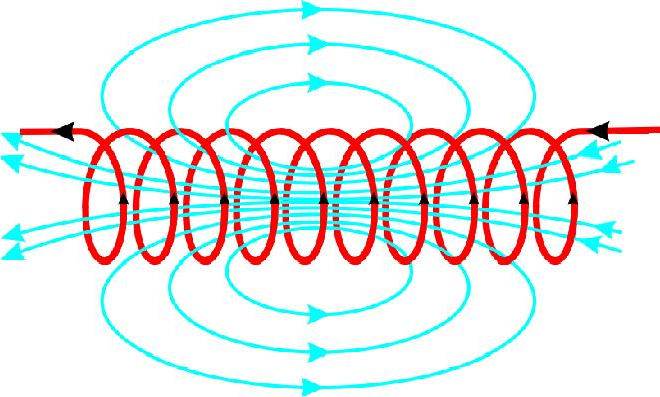
\includegraphics[height=3.8cm]{solenoid_field.png}};
  \node[anchor=north west,text width=9.4cm,font=\sffamily,align=left] at ([xshift=1.8cm,yshift=-10.8cm]current page.north west) {%
    {\large\bfseries Practise the way the exam asks.}\\[6pt]
    \small Every topic of the chapter, turned into questions you answer in this book:
    fill in the blanks, label and draw field lines, apply the hand rules, complete the
    derivation, solve the numerical, explain the reason. Each unit ends with a self check,
    and the book ends with a full 40-mark chapter test.\\[10pt]
    \faStar\ Marks badges: \badge{1M} \badge{2M} \badge{4M}\\[4pt]
    \faStar\ Academic standards: \asbadge{AS1} concept \asbadge{AS3} experiment \asbadge{AS5} diagram \asbadge{AS7} application\\[4pt]
    \faStar\ \tb\ marks every question from \emph{Improve your learning}};
  \node[anchor=south west,font=\sffamily] at ([xshift=1.8cm,yshift=2.2cm]current page.south west) {%
    \renewcommand{\arraystretch}{2.1}
    \begin{tabular}{@{}l@{\quad}p{8.5cm}@{}}
    \textbf{Name} & \hrulefill\\
    \textbf{Class / Section} & \hrulefill\\
    \textbf{Roll No.} & \hrulefill\\
    \textbf{School} & \hrulefill\\
    \end{tabular}};
\end{tikzpicture}
\null\clearpage

% =====================================================================
\section*{\sffamily\color{ecblue}How to use this workbook}
\begin{enumerate}[label=\textcolor{ecorange}{\faArrowRight},leftmargin=6mm]
\item Read the \textbf{Recall in 60 seconds} box first. If a point feels new, go back to the textbook page before you start.
\item Answer in the book, in pen. Do the questions \textbf{without} looking at the textbook, then check.
\item Numericals: \emph{formula $\rightarrow$ values in SI units (m, m$^2$, A, T) $\rightarrow$ answer with unit}.
\item Field-line diagrams: draw in pencil, put \textbf{arrows on every line}, mark N and S, $\odot$ and $\otimes$.
\item For every direction question, write which \textbf{rule} you used (thumb rule, right hand rule, Lenz's law).
\item Fill in the \textbf{Self check} after each unit; copy mistakes into the \textbf{Mistake log}.
\end{enumerate}

\subsection*{\sffamily\color{ecblue}What the exam asks from this chapter}
\renewcommand{\arraystretch}{1.35}
\begin{tabularx}{\linewidth}{>{\bfseries\sffamily}p{1.6cm}X}
\toprule
\rowcolor{ecblue}\textcolor{white}{Marks} & \textcolor{white}{\textbf{\sffamily Typical questions}}\\
\midrule
1 mark & Units (weber, tesla), one-line laws, energy change in motor/generator, force when parallel to $B$, MCQs.\\
2 marks & Direction of current/field/force from a figure, pole of a coil, TV distortion, closed field lines, short numericals on $B=\Phi/A$, $F=ILB$, $\varepsilon=Blv$, $\varepsilon=N\Delta\Phi/\Delta t$.\\
4 marks & Activities: current produces a field; force on a wire; Faraday's law. Working of motor and generators. Derivation of $\varepsilon=Blv$, $F=ILB$, $r=mv/Bq$. Lenz's law with energy argument. Levitation.\\
Diagrams & Field lines of bar magnet, straight wire, solenoid; right hand rules; coil in a field; motor; Faraday's activity; AC generator and emf graph.\\
\bottomrule
\end{tabularx}

\subsection*{\sffamily\color{ecblue}My progress tracker}
\renewcommand{\arraystretch}{1.55}
\begin{tabularx}{\linewidth}{>{\sffamily}l X c c c}
\toprule
\rowcolor{ecteal!15}\textbf{Unit} & \textbf{Topic} & \textbf{Score} & \textbf{Confidence} & \textbf{Revised on}\\
\midrule
1 & Oersted, magnetic field and field lines & \rule{1.3cm}{0.3pt} & \tick\,\tick\,\tick & \rule{1.6cm}{0.3pt}\\
2 & Magnetic flux and flux density & \rule{1.3cm}{0.3pt} & \tick\,\tick\,\tick & \rule{1.6cm}{0.3pt}\\
3 & Fields of a wire, coil and solenoid & \rule{1.3cm}{0.3pt} & \tick\,\tick\,\tick & \rule{1.6cm}{0.3pt}\\
4 & Force on a moving charge & \rule{1.3cm}{0.3pt} & \tick\,\tick\,\tick & \rule{1.6cm}{0.3pt}\\
5 & Force on a current; electric motor & \rule{1.3cm}{0.3pt} & \tick\,\tick\,\tick & \rule{1.6cm}{0.3pt}\\
6 & Induction: Faraday, Lenz, motional emf & \rule{1.3cm}{0.3pt} & \tick\,\tick\,\tick & \rule{1.6cm}{0.3pt}\\
7 & Applications, levitation, generators & \rule{1.3cm}{0.3pt} & \tick\,\tick\,\tick & \rule{1.6cm}{0.3pt}\\
-- & One-mark rapid fire & \rule{1.3cm}{0.3pt} & \tick\,\tick\,\tick & \rule{1.6cm}{0.3pt}\\
-- & Chapter test (40 marks) & \rule{1.3cm}{0.3pt} & \tick\,\tick\,\tick & \rule{1.6cm}{0.3pt}\\
\bottomrule
\end{tabularx}
{\small Confidence: tick one box for ``shaky'', two for ``fine'', three for ``I can teach it''.}

% =====================================================================
\unit{Magnetic field and field lines}{\badge{1M}\ \badge{2M}\ \badge{4M}}
% =====================================================================
\begin{recall}
\begin{itemize}[leftmargin=5mm,itemsep=0pt]
\item \key{Oersted (1820)}: a compass needle under a wire deflects when current flows $\Rightarrow$ a current produces a magnetic field.
\item A \key{magnetic field} is the region around a magnet where its force acts without contact. It has \textbf{strength} and \textbf{direction} and is three-dimensional.
\item \key{Field lines} are imaginary; the \textbf{tangent} gives the direction; crowded lines = strong field. Outside a magnet they go N $\to$ S. Uniform field: parallel, equally spaced lines.
\end{itemize}
\end{recall}

\exhead{A}{Fill in the blanks}{\asbadge{AS1}\ \badge{1M}}
\begin{enumerate}
\item The scientist who first showed that a current deflects a compass needle was \blank{Oersted}.
\item The direction of the field at a point is given by the \blank{tangent} to the field line at that point.
\item Field lines are \blank{crowded} near the poles, where the field is \blank{strong}.
\item A field whose strength and direction are the same everywhere is called a \blank{uniform} field.
\item Outside a bar magnet field lines go from \blank[1.5cm]{N} to \blank[1.5cm]{S}.
\end{enumerate}

\exhead{B}{True or false}{\asbadge{AS1}\ \badge{1M}}
{\small Write T or F. If false, correct it on the line below.}
\begin{enumerate}
\tf{Field lines of a magnet can cross each other.}{F}{They never cross; at a crossing the field would have two directions, which is impossible.}
\ifanswers\else\writelines{1}\fi
\tf{The magnetic field of a bar magnet exists only in the plane of the paper.}{F}{It is three-dimensional; it surrounds the magnet in all directions.}
\ifanswers\else\writelines{1}\fi
\tf{Far from a magnet a compass needle points almost north--south.}{T}{}
\ifanswers\else\writelines{1}\fi
\end{enumerate}

\exhead{C}{Label the Oersted apparatus}{\asbadge{AS5}\ \badge{2M}}
\begin{center}
\figlab{oersted_setup.png}{width=0.62\linewidth}{
\draw[fptr] (0.18,1.12) node[flab,anchor=south]{(a) \blank[2.3cm]{copper wire}} -- (0.36,0.82);
\draw[fptr] (0.85,1.12) node[flab,anchor=south]{(b) \blank[2.3cm]{battery}} -- (0.66,0.78);
\draw[fptr] (0.20,0.05) node[flab,anchor=north]{(c) \blank[2.3cm]{compass}} -- (0.40,0.60);
\draw[fptr] (0.72,0.05) node[flab,anchor=north]{(d) \blank[2.3cm]{key}} -- (0.54,0.40);}
\end{center}
\vspace{6pt}
\begin{enumerate}
\item What happens to the needle when the key is closed? What does it prove? \mk{2M}
\answer[3]{The needle deflects. When the key is opened it returns to the north--south direction. This proves that a current-carrying wire produces a magnetic field around it: electricity and magnetism are related.}
\end{enumerate}

\exhead{D}{Draw field lines}{\asbadge{AS5}\ \badge{2M}}
Draw at least six field lines of the bar magnet below, with arrows. \mk{2M}
\begin{center}
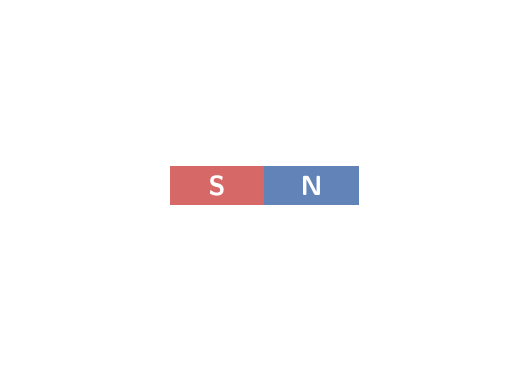
\begin{tikzpicture}
\fill[ecred!70] (-1.2,-0.25) rectangle (0,0.25); \fill[ecblue!70] (0,-0.25) rectangle (1.2,0.25);
\node[white,font=\sffamily\bfseries] at (-0.6,0) {S}; \node[white,font=\sffamily\bfseries] at (0.6,0) {N};
\ifanswers
\foreach \h in {0.8,1.4,2.1}{
  \draw[afl=0.5] (1.2,0.1) .. controls (2.5,\h) and (-2.5,\h) .. (-1.2,0.1);
  \draw[afl=0.5] (1.2,-0.1) .. controls (2.5,-\h) and (-2.5,-\h) .. (-1.2,-0.1);}
\draw[afl=0.5] (1.2,0) -- (3,0); \draw[afl=0.5] (-3,0) -- (-1.2,0);
\else
\draw[white] (-3,-2) rectangle (3,2);
\fi
\end{tikzpicture}
\end{center}

\exhead{E}{Short answers}{\tb\ \asbadge{AS1}\ \badge{2M}}
\begin{enumerate}
\item Are magnetic field lines closed? Explain. \mk{2M}
\answer[4]{Yes. Around a straight wire they are complete circles. For a solenoid (and a bar magnet) the lines outside go from N to S and continue inside from S to N, so every line is a closed loop.}
\item How can you find the strength and the direction of a magnetic field using field lines? \mk{2M}
\answer[3]{Direction: the tangent to the field line at the point (the way a compass needle points). Strength: how close the lines are; crowded lines mean a strong field, widely spaced lines a weak field.}
\end{enumerate}

\selfcheck{19}{
\item describe Oersted's experiment and its conclusion
\item state the properties of field lines
\item draw the field lines of a bar magnet with arrows}

% =====================================================================
\unit{Magnetic flux and flux density}{\badge{1M}\ \badge{2M}}
% =====================================================================
\begin{recall}
\begin{itemize}[leftmargin=5mm,itemsep=0pt]
\item \key{Magnetic flux} $\Phi$: number of field lines through a plane held perpendicular to the field. Unit \imp{weber (Wb)}.
\item \key{Flux density} $B=\dfrac{\Phi}{A}$ (area perpendicular to the field). Unit \imp{Wb/m$^2$ = tesla (T)}.
\item Plane tilted so its normal makes $\theta$ with $B$: effective area $A\cos\theta$, so \imp{$\Phi=BA\cos\theta$}. Plane parallel to $B$: $\Phi=0$.
\end{itemize}
\end{recall}

\exhead{A}{Fill in the blanks}{\asbadge{AS1}\ \badge{1M}}
\begin{enumerate}
\item The SI unit of magnetic flux is the \blank{weber}.
\item The SI unit of magnetic flux density is the \blank{tesla}, which equals \blank{Wb/m$^2$}.
\item Magnetic flux density is also called magnetic \blank{induction}.
\item The flux through a plane held parallel to the field is \blank[1.5cm]{zero}.
\end{enumerate}

\exhead{B}{Complete the derivation of $\Phi=BA\cos\theta$}{\asbadge{AS1}\ \badge{2M}}
\noindent
\begin{minipage}[c]{0.38\linewidth}\centering
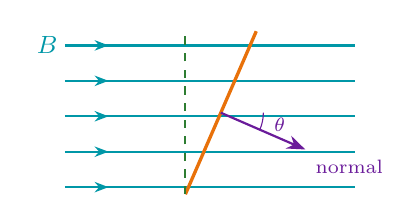
\begin{tikzpicture}[scale=0.9]
\foreach \y in {0.2,0.7,1.2,1.7,2.2} \draw[fl=0.15] (-0.5,\y) -- (3.6,\y);
\node[font=\small\bfseries,fieldc] at (-0.75,2.2) {$B$};
\draw[very thick,ecorange] (1.2,0.1) -- (2.2,2.4);
\coordinate (C) at (1.7,1.25);
\draw[-{Stealth},thick,ecpurple] (C) -- ($(C)+(-23.5:1.3)$) node[below right,font=\scriptsize]{normal};
\draw[ecpurple] ($(C)+(0.6,0)$) arc (0:-23.5:0.6); \node[font=\scriptsize,ecpurple] at ($(C)+(-12:0.85)$) {$\theta$};
\draw[thick,dashed,ecgreen] (1.2,0.1) -- (1.2,2.4);
\end{tikzpicture}\\{\small edge view of a plane of area $A$}
\end{minipage}\hfill
\begin{minipage}[c]{0.58\linewidth}
(1) $B$ uses the area \blank{perpendicular} to the field:\\ \hspace*{6mm}$B=\dfrac{\Phi}{A_\perp}$\\[4pt]
(2) The effective area perpendicular to the field is $A_\perp=\mblank{A\cos\theta}$.\\[4pt]
(3) So $B=\mblank[2.2cm]{\dfrac{\Phi}{A\cos\theta}}$ and $\Phi=\mblank[2.2cm]{BA\cos\theta}$.\\[4pt]
(4) $\theta=0^\circ$: $\Phi=\mblank{BA}$;\quad $\theta=90^\circ$: $\Phi=\mblank{0}$.
\end{minipage}

\exhead{C}{Numericals}{\asbadge{AS7}\ \badge{2M}}
\begin{worked}[Worked example: 0.02 Wb crosses 0.4 m$^2$ normally]
$B=\dfrac{\Phi}{A}=\dfrac{0.02}{0.4}=0.05$ T.\quad \textbf{Always} convert cm$^2$ to m$^2$ (1 cm$^2=10^{-4}$ m$^2$).
\end{worked}
\begin{enumerate}
\item $B=0.8$ T passes normally through a loop of area 0.05 m$^2$. Find the flux. \mk{2M}
\answer[2]{$\Phi=BA=0.8\times0.05=0.04$ Wb.}
\item The same loop is turned so that its normal makes $60^\circ$ with the field. Find the new flux. \mk{2M}
\answer[2]{$\Phi=BA\cos60^\circ=0.04\times\frac12=0.02$ Wb.}
\item A flux of $6\times10^{-4}$ Wb passes normally through 20 cm$^2$. Find $B$. \mk{2M}
\answer[3]{$A=20\times10^{-4}=2\times10^{-3}$ m$^2$. $B=\dfrac{6\times10^{-4}}{2\times10^{-3}}=0.3$ T.}
\end{enumerate}

\selfcheck{15}{
\item define magnetic flux and flux density with units
\item derive $\Phi=BA\cos\theta$ and use its special cases
\item convert areas to m$^2$ in numericals}

% =====================================================================
\unit{Fields of a wire, a coil and a solenoid}{\badge{1M}\ \badge{2M}\ \badge{4M}}
% =====================================================================
\begin{recall}
\begin{itemize}[leftmargin=5mm,itemsep=0pt]
\item \key{Straight wire}: field lines are concentric circles. \textbf{Right hand thumb rule}: thumb along current, curled fingers give the field. Out of the page $\odot$ $\Rightarrow$ anticlockwise; into the page $\otimes$ $\Rightarrow$ clockwise.
\item \key{Circular coil}: field at the centre is perpendicular to the plane of the coil. Curl fingers along the current, thumb gives $B$. Anticlockwise current (as seen) $\Rightarrow$ that face is \textbf{N}.
\item \key{Solenoid}: behaves like a bar magnet; outside N $\to$ S, inside S $\to$ N; lines are closed loops.
\end{itemize}
\end{recall}

\exhead{A}{Draw the field lines}{\asbadge{AS5}\ \badge{2M}}
Draw three field lines with arrows around each wire. \mk{2M}
\begin{center}
\begin{tabular}{c@{\hspace{2cm}}c}
\begin{tikzpicture}
\ifanswers\foreach \r in {0.5,0.9,1.3} \draw[anscol,thick,postaction={decorate},decoration={markings,mark=at position 0.25 with {\arrow{Stealth[length=5pt]}},mark=at position 0.75 with {\arrow{Stealth[length=5pt]}}}] (0,0) circle (\r);
\else\draw[white] (-1.4,-1.4) rectangle (1.4,1.4);\fi
\outpage{(0,0)}
\end{tikzpicture} &
\begin{tikzpicture}
\ifanswers\foreach \r in {0.5,0.9,1.3} \draw[anscol,thick,postaction={decorate},decoration={markings,mark=at position 0.25 with {\arrowreversed{Stealth[length=5pt]}},mark=at position 0.75 with {\arrowreversed{Stealth[length=5pt]}}}] (0,0) circle (\r);
\else\draw[white] (-1.4,-1.4) rectangle (1.4,1.4);\fi
\inpage{(0,0)}
\end{tikzpicture}\\
(1) current out of the page & (2) current into the page\\
\ifanswers{\small\color{anscol}anticlockwise}\fi & \ifanswers{\small\color{anscol}clockwise}\fi\\
\end{tabular}
\end{center}

\exhead{B}{Direction questions from the textbook}{\tb\ \asbadge{AS1}\ \badge{1M}\ \badge{2M}}
\noindent
\begin{minipage}[t]{0.22\linewidth}\centering
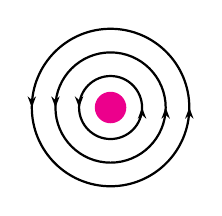
\begin{tikzpicture}[scale=0.5]
\foreach \r in {0.8,1.4,2.0} \draw[thick,postaction={decorate},decoration={markings,mark=at position 0.0 with {\arrow{Stealth[length=4pt]}},mark=at position 0.5 with {\arrow{Stealth[length=4pt]}}}] (0,0) circle (\r);
\fill[magenta] (0,0) circle (0.4);
\end{tikzpicture}\\{\small fig-Q1}
\end{minipage}\hfill
\begin{minipage}[t]{0.75\linewidth}
\begin{enumerate}
\item Field lines around a wire are shown in fig-Q1 (anticlockwise). What is the direction of the current? \mk{1M}
\answer[2]{Out of the page (towards the reader), by the right hand thumb rule.}
\end{enumerate}
\end{minipage}\\[6pt]
\begin{minipage}[t]{0.22\linewidth}\centering
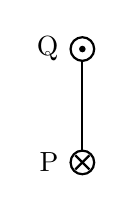
\begin{tikzpicture}[scale=0.6]
\draw[thick] (0,-1) -- (0,1);
\outpage[0.25]{(0,1.2)} \node[left] at (-0.3,1.2) {Q};
\inpage[0.25]{(0,-1.2)} \node[left] at (-0.3,-1.2) {P};
\end{tikzpicture}\\{\small fig-Q3}
\end{minipage}\hfill
\begin{minipage}[t]{0.75\linewidth}
\begin{enumerate}[start=2]
\item A coil is kept perpendicular to the page. At P the current flows into the page, at Q it comes out (fig-Q3). What is the direction of the field due to the coil? \mk{2M}
\answer[3]{At the centre, the wire at P (into page, clockwise field) gives a field to the right; the wire at Q (out of page, anticlockwise field) also gives a field to the right. So the field is along the axis of the coil, from left to right, perpendicular to the plane of the coil.}
\end{enumerate}
\end{minipage}\\[6pt]
\begin{minipage}[t]{0.22\linewidth}\centering
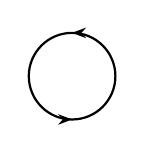
\begin{tikzpicture}[scale=0.55]
\draw[thick,postaction={decorate},decoration={markings,mark=at position 0.25 with {\arrow{Stealth[length=5pt]}},mark=at position 0.75 with {\arrow{Stealth[length=5pt]}}}] (0,0) circle (1);
\end{tikzpicture}\\{\small fig-Q4}
\end{minipage}\hfill
\begin{minipage}[t]{0.75\linewidth}
\begin{enumerate}[start=3]
\item The current in a coil flows as in fig-Q4 (anticlockwise as you see it). What pole is formed at this face? \mk{1M}
\answer[2]{North pole: curling the right-hand fingers anticlockwise, the thumb (field) points towards the viewer.}
\end{enumerate}
\end{minipage}

\exhead{C}{Label the solenoid}{\asbadge{AS5}\ \badge{2M}}
In the figure the current enters at the right end and leaves at the left. Mark the N and S ends and the direction of the field inside.
\begin{center}
\figlab{solenoid_field.png}{width=0.55\linewidth}{
\node[font=\sffamily\bfseries] at (-0.06,0.5) {\ifanswers\textcolor{anscol}{N}\else\fbox{\phantom{N}}\fi};
\node[font=\sffamily\bfseries] at (1.06,0.5) {\ifanswers\textcolor{anscol}{S}\else\fbox{\phantom{S}}\fi};
\ifanswers\draw[-{Stealth[length=6pt]},anscol,very thick] (0.75,0.5) -- (0.25,0.5) node[midway,below=6pt,font=\small]{inside: S $\to$ N};\fi}
\end{center}

\exhead{D}{Experiment}{\tb\ \asbadge{AS3}\ \badge{4M}}
Explain with the help of two activities that a current-carrying wire produces a magnetic field. \mk{4M}
\answer[12]{\textbf{Activity 1 (Oersted):} a wire stretched through the slits of two sticks is connected to a battery through a key; a compass is placed below it. When the key is closed the needle deflects; when it is opened the needle returns to N--S.\\
\textbf{Activity 4:} a vertical wire passes through a hole in a plank; 6--10 compass needles are placed on a circle around it. When the current flows, the needles set along tangents to the circle; iron filings sprinkled around form concentric circles.\\
\textbf{Conclusion:} the wire produces a magnetic field whose lines are concentric circles around it; the direction is given by the right hand thumb rule.}

\selfcheck{20}{
\item draw the field of a straight wire for both current directions
\item find the pole of a coil face from the current direction
\item describe the field of a solenoid and why its lines are closed loops}

% =====================================================================
\unit{Force on a moving charge}{\badge{1M}\ \badge{2M}\ \badge{4M}}
% =====================================================================
\begin{recall}
\begin{itemize}[leftmargin=5mm,itemsep=0pt]
\item A magnet distorts the picture on a CRT TV: the field exerts a force on the moving electrons.
\item \imp{$F=qvB\sin\theta$}; $F=qvB$ when $v\perp B$; $F=0$ when $v\parallel B$ or $v=0$.
\item Direction: right hand rule (forefinger $v$, middle finger $B$, thumb $F$), for a \textbf{positive} charge; reverse it for an electron. $F$ is always perpendicular to both $v$ and $B$.
\item A charge moving $\perp B$ goes round a circle: $r=\dfrac{mv}{Bq}$, $T=\dfrac{2\pi m}{Bq}$.
\end{itemize}
\end{recall}

\exhead{A}{Fill in the blanks}{\asbadge{AS1}\ \badge{1M}}
\begin{enumerate}
\item The force on a charge moving parallel to the field is \blank[1.5cm]{zero}.
\item The magnetic force is always perpendicular to both the \blank{velocity} and the \blank{field}.
\item For an electron, the direction of force is \blank{opposite} to that found for a positive charge.
\item The magnetic force on a charge moving $\perp B$ acts as the \blank{centripetal} force.
\end{enumerate}

\exhead{B}{Complete the derivation}{\asbadge{AS1}\ \badge{4M}}
A charge $q$ of mass $m$ moves with speed $v$ perpendicular to a uniform field $B$.\\[4pt]
(1) Magnetic force: $F=\mblank{qvB}$ \quad(since $\sin90^\circ=\mblank[1cm]{1}$).\\[4pt]
(2) This force is always perpendicular to the velocity, so the path is a \blank{circle}.\\[4pt]
(3) Centripetal force = magnetic force: \quad $\mblank{\dfrac{mv^2}{r}}=qvB$ \quad$\Rightarrow$\quad $r=\mblank[2cm]{\dfrac{mv}{Bq}}$\\[4pt]
(4) Time period $T=\dfrac{2\pi r}{v}=\mblank[2.2cm]{\dfrac{2\pi m}{Bq}}$, which does \blank{not} depend on the speed.

\exhead{C}{Numericals}{\asbadge{AS7}\ \badge{2M}}
\begin{enumerate}
\item A charge of $2\times10^{-6}$ C moves at $3\times10^4$ m/s perpendicular to $B=0.5$ T. Find the force. \mk{2M}
\answer[2]{$F=qvB=2\times10^{-6}\times3\times10^4\times0.5=3\times10^{-2}$ N.}
\item The same charge moves at $30^\circ$ to the field. Find the force. \mk{2M}
\answer[2]{$F=qvB\sin30^\circ=0.03\times\frac12=1.5\times10^{-2}$ N.}
\item A proton ($m=1.67\times10^{-27}$ kg, $q=1.6\times10^{-19}$ C) moves at $10^6$ m/s perpendicular to $B=1$ T. Find the radius of its path. \mk{2M}
\answer[3]{$r=\dfrac{mv}{Bq}=\dfrac{1.67\times10^{-27}\times10^6}{1\times1.6\times10^{-19}}=1.04\times10^{-2}$ m $\approx1$ cm.}
\end{enumerate}

\exhead{D}{Short answers}{\tb\ \asbadge{AS1}\ \badge{2M}}
\begin{enumerate}
\item Why does the picture appear distorted when a bar magnet is brought close to the screen of a television? \mk{2M}
\answer[3]{The picture on a CRT screen is made by a beam of fast-moving electrons. The magnet's field exerts a force $F=qvB\sin\theta$ on them, which changes their path, so they strike the wrong spots and the picture is distorted.}
\item State the right hand rule for the direction of force on a positive charge. \mk{2M}
\answer[3]{Stretch the thumb, forefinger and middle finger of the right hand mutually perpendicular. If the forefinger points along the velocity (or current) and the middle finger along the field, the thumb gives the direction of the force.}
\end{enumerate}

\selfcheck{25}{
\item use $F=qvB\sin\theta$ including the zero-force cases
\item find the direction of force with the right hand rule, and reverse it for electrons
\item derive $r=mv/Bq$ and $T=2\pi m/Bq$}

% =====================================================================
\unit{Force on a current; electric motor}{\badge{1M}\ \badge{2M}\ \badge{4M}}
% =====================================================================
\begin{recall}
\begin{itemize}[leftmargin=5mm,itemsep=0pt]
\item A current is moving charge, so a current-carrying wire in a field feels a force: \imp{$F=ILB\sin\theta$}; $F=ILB$ when $I\perp B$; $F=0$ when $I\parallel B$.
\item Activity 8: a wire in a horseshoe magnet is deflected; reversing the current or the poles reverses the deflection.
\item \key{Motor}: forces on opposite sides of a coil are equal and opposite (net force 0) but form a \textbf{couple} that rotates the coil. \textbf{Split rings} and brushes reverse the current every half turn. Electrical $\to$ mechanical energy.
\end{itemize}
\end{recall}

\exhead{A}{Complete the derivation of $F=ILB$}{\asbadge{AS1}\ \badge{4M}}
(1) Force on one charge moving with drift velocity $v$ perpendicular to $B$: $F_0=\mblank{qvB}$.\\[4pt]
(2) Total charge in the length $L$ inside the field is $Q$: $F=\mblank{QvB}$ \dots(1)\\[4pt]
(3) Time to cross length $L$: $t=\dfrac{L}{v}$, so $v=\mblank{\dfrac{L}{t}}$ \dots(2)\\[4pt]
(4) Put (2) in (1): $F=\mblank[2.2cm]{\dfrac{Q}{t}LB}$ \dots(3)\\[4pt]
(5) Since $\dfrac{Q}{t}=\mblank[1cm]{I}$, \quad $F=\mblank[1.6cm]{ILB}$. At an angle $\theta$: $F=\mblank[2cm]{ILB\sin\theta}$.

\exhead{B}{Numericals}{\tb\ \asbadge{AS7}\ \badge{2M}}
\begin{enumerate}
\item \tb\ An 8 N force acts on a 20 cm conductor placed perpendicular to a magnetic field. The current is 40 A. Find the magnetic field induction. \mk{2M}
\answer[3]{$L=0.2$ m. $B=\dfrac{F}{IL}=\dfrac{8}{40\times0.2}=1$ T.}
\item A wire 0.5 m long carries 4 A at $30^\circ$ to a field of 0.2 T. Find the force. \mk{2M}
\answer[2]{$F=ILB\sin30^\circ=4\times0.5\times0.2\times\frac12=0.2$ N.}
\end{enumerate}

\exhead{C}{Direction of force}{\tb\ \asbadge{AS1}\ \badge{2M}}
\noindent
\begin{minipage}[c]{0.3\linewidth}\centering
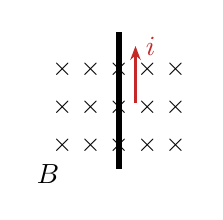
\begin{tikzpicture}[scale=0.6]
\foreach \x in {-2,...,2}{\foreach \y in {-1,...,1}{\node[font=\small] at (\x*0.6,\y*0.8) {$\times$};}}
\draw[line width=2pt] (0,-1.3) -- (0,1.6);
\draw[cur] (0.35,0.1) -- (0.35,1.3) node[right]{$i$};
\node at (-1.5,-1.4) {$B$};
\end{tikzpicture}\\{\small fig-Q5}
\end{minipage}\hfill
\begin{minipage}[c]{0.67\linewidth}
A straight wire carrying current $i$ upward is kept perpendicular to a field directed into the page; length $L$ is in the field. Find the magnitude and direction of the force. \mk{2M}
\answer[3]{Magnitude $F=iLB$ (since $\theta=90^\circ$). Right hand rule: forefinger up ($i$), middle finger into the page ($B$) $\Rightarrow$ thumb points to the \textbf{left}. The force acts to the left, in the plane of the page.}
\end{minipage}

\exhead{D}{Motor}{\asbadge{AS1}\ \asbadge{AS5}\ \badge{4M}}
\noindent
\begin{minipage}[c]{0.38\linewidth}\centering
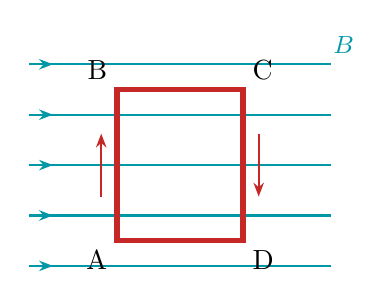
\begin{tikzpicture}[scale=0.8]
\foreach \y in {-1.6,-0.8,0,0.8,1.6} \draw[fl=0.08] (-2.4,\y) -- (2.4,\y);
\node[font=\small\bfseries,fieldc] at (2.6,1.9) {$B$};
\draw[ecred,line width=2pt] (-1,-1.2) -- (-1,1.2) -- (1,1.2) -- (1,-1.2) -- cycle;
\draw[cur] (-1.25,-0.5) -- (-1.25,0.5); \draw[cur] (1.25,0.5) -- (1.25,-0.5);
\node[below left] at (-1,-1.2) {A}; \node[above left] at (-1,1.2) {B};
\node[above right] at (1,1.2) {C}; \node[below right] at (1,-1.2) {D};
\end{tikzpicture}
\end{minipage}\hfill
\begin{minipage}[c]{0.6\linewidth}
\begin{enumerate}
\item The force on AB is directed \blank{into the page} and on CD \blank{out of the page}.\mk{1M}
\item The net force on the coil is \blank[1.5cm]{zero}, yet the coil \blank{rotates} because the two forces form a \blank{couple}. \mk{1M}
\item Why is the current reversed every half turn, and which part does it? \mk{2M}
\answer[3]{After half a turn the forces would turn the coil back, so it would only rock to and fro. The split rings (commutator), rotating with the coil, swap brushes every half turn, reversing the current so the rotation continues in the same direction.}
\end{enumerate}
\end{minipage}

\exhead{E}{Experiment}{\tb\ \asbadge{AS3}\ \badge{4M}}
How do you verify experimentally that a current-carrying conductor experiences a force when kept in a magnetic field? \mk{4M}
\answer[10]{\textbf{Materials:} wooden plank, two split sticks, copper wire, 9 V battery, switch, horseshoe magnet.\\
\textbf{Procedure:} pass the wire through the splits of the sticks and connect it to the battery through the switch. Close the switch and bring the horseshoe magnet so the wire lies between its poles.\\
\textbf{Observation:} the wire is deflected (pushed up or down). Reversing the poles of the magnet, or the direction of the current, reverses the deflection.\\
\textbf{Conclusion:} a current-carrying conductor in a field experiences a force $F=ILB$; its direction is given by the right hand rule.}

\selfcheck{27}{
\item derive $F=ILB$ from $F=qvB$
\item find the direction of force on a wire with the right hand rule
\item explain the working of a motor, including split rings}

% =====================================================================
\unit{Induction: Faraday, Lenz and motional emf}{\badge{1M}\ \badge{2M}\ \badge{4M}}
% =====================================================================
\begin{recall}
\begin{itemize}[leftmargin=5mm,itemsep=0pt]
\item \key{Electromagnetic induction}: a current is induced in a coil when the flux through it changes (relative motion of magnet and coil).
\item \key{Faraday's law}: $\varepsilon=\dfrac{\Delta\Phi}{\Delta t}$; for $N$ turns $\varepsilon=N\dfrac{\Delta\Phi_0}{\Delta t}$.
\item \key{Lenz's law}: the induced current opposes the change in flux (conservation of energy). N pole approaching $\Rightarrow$ near face of coil becomes N.
\item \key{Motional emf}: $\varepsilon=Blv$ for a conductor of length $l$ moving with speed $v$ perpendicular to $B$.
\end{itemize}
\end{recall}

\exhead{A}{Activity 9: what does the galvanometer show?}{\asbadge{AS3}\ \badge{1M}}
\renewcommand{\arraystretch}{1.7}
\begin{tabularx}{\linewidth}{>{\small}X>{\small}X}
\toprule
\rowcolor{ecblue}\textcolor{white}{\textbf{Action}} & \textcolor{white}{\textbf{Galvanometer}}\\
\midrule
Magnet held at rest inside the coil & \blank{no deflection}\\
N pole pushed towards the coil & \blank{deflects one way}\\
N pole pulled away from the coil & \blank{deflects the opposite way}\\
S pole pushed towards the coil & \blank{deflects opposite to N pushed in}\\
Magnet pushed in faster & \blank{larger deflection}\\
\bottomrule
\end{tabularx}

\exhead{B}{Fill in the blanks}{\asbadge{AS1}\ \badge{1M}}
\begin{enumerate}
\item The current produced by changing flux is called the \blank{induced current}.
\item Lenz's law is a consequence of the conservation of \blank{energy}.
\item When the N pole of a magnet approaches a coil, the face of the coil nearer to it becomes a \blank[1.5cm]{north} pole.
\item $\varepsilon=Blv$ is called the \blank{motional emf}.
\end{enumerate}

\exhead{C}{Complete the derivation of $\varepsilon=Blv$}{\asbadge{AS1}\ \badge{4M}}
A cross wire of length $l$ lies on two parallel conductors in a uniform field $B$. It is moved a distance $s$ in time $\Delta t$ and a current $I$ flows.\\[4pt]
(1) Force of the field on the cross wire: $F=\mblank{BIl}$ \dots(8)\\[4pt]
(2) Work done by us in moving it: $W=Fs=\mblank{BIls}$ \dots(9)\\[4pt]
(3) Change in flux as the loop area changes by $ls$: $\Delta\Phi=\mblank{Bls}$ \dots(10) \;$\Rightarrow W=\mblank{I\,\Delta\Phi}$\\[4pt]
(4) Dividing by $\Delta t$: $P=\dfrac{W}{\Delta t}=\mblank{\dfrac{I\Delta\Phi}{\Delta t}}$; comparing with $P=\varepsilon I$ gives $\varepsilon=\mblank{\dfrac{\Delta\Phi}{\Delta t}}$\\[4pt]
(5) Also $P=Fv=\mblank{BIlv}$ (since $\dfrac{s}{\Delta t}=v$). So $\varepsilon I=BIlv$ \;$\Rightarrow\;\varepsilon=\mblank[1.6cm]{Blv}$

\exhead{D}{Numericals}{\tb\ \asbadge{AS7}\ \badge{2M}}
\begin{worked}[Worked example (textbook): 400 turns, flux per turn rises by 0.001 Wb in 0.1 s]
$\varepsilon=N\dfrac{\Delta\Phi_0}{\Delta t}=\dfrac{400\times0.001}{0.1}=4$ V. While the flux stays constant (0.1 s to 0.3 s), $\varepsilon=0$.
\end{worked}
\begin{enumerate}
\item \tb\ Find the length of a conductor moving at 10 m/s perpendicular to a field of 0.8 T if it induces an emf of 8 V. \mk{2M}
\answer[2]{$l=\dfrac{\varepsilon}{Bv}=\dfrac{8}{0.8\times10}=1$ m.}
\item The flux per turn in a coil of 100 turns falls from 0.05 Wb to 0.01 Wb in 0.2 s. Find the induced emf. \mk{2M}
\answer[3]{$\Delta\Phi_0=0.04$ Wb. $\varepsilon=\dfrac{100\times0.04}{0.2}=20$ V.}
\item A 1.5 m rod moves at 2 m/s perpendicular to $B=0.4$ T. Find the emf. \mk{2M}
\answer[2]{$\varepsilon=Blv=0.4\times1.5\times2=1.2$ V.}
\end{enumerate}

\exhead{E}{Figure questions}{\tb\ \asbadge{AS1}\ \asbadge{AS2}\ \badge{2M}}
\noindent
\begin{minipage}[c]{0.3\linewidth}\centering
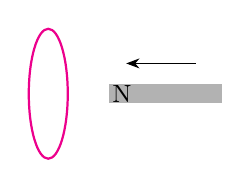
\begin{tikzpicture}[scale=0.55]
\draw[magenta,thick] (0,0) ellipse (0.45 and 1.5);
\fill[gray!60] (1.4,-0.22) rectangle (4,0.22); \node[font=\small] at (1.7,0) {N};
\draw[-{Stealth}] (3.4,0.7) -- (1.8,0.7);
\end{tikzpicture}\\{\small fig-Q2}
\end{minipage}\hfill
\begin{minipage}[c]{0.67\linewidth}
\begin{enumerate}
\item A bar magnet with its N pole facing a coil moves towards it (fig-Q2). What happens to the flux through the coil? Which way does the induced current flow as seen from the magnet? \mk{2M}
\answer[3]{The flux through the coil increases. By Lenz's law the near face becomes N to repel the magnet, so the induced current is anticlockwise as seen from the magnet.}
\end{enumerate}
\end{minipage}\\[6pt]
\begin{minipage}[c]{0.3\linewidth}\centering
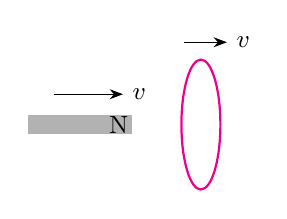
\begin{tikzpicture}[scale=0.55]
\fill[gray!60] (-3,-0.22) rectangle (-0.6,0.22); \node[font=\small] at (-0.9,0) {N};
\draw[-{Stealth}] (-2.4,0.7) -- (-0.8,0.7) node[right,font=\small]{$v$};
\draw[magenta,thick] (1,0) ellipse (0.45 and 1.5);
\draw[-{Stealth}] (0.6,1.9) -- (1.6,1.9) node[right,font=\small]{$v$};
\end{tikzpicture}\\{\small fig-Q6}
\end{minipage}\hfill
\begin{minipage}[c]{0.67\linewidth}
\begin{enumerate}[start=2]
\item \tb\ The coil and the bar magnet both move in the same direction with the same speed (fig-Q6). What happens? \mk{2M}
\answer[3]{There is no relative motion between the magnet and the coil, so the flux through the coil does not change. No emf is induced and no current flows.}
\end{enumerate}
\end{minipage}

\exhead{F}{Long answers}{\tb\ \asbadge{AS1}\ \asbadge{AS3}\ \badge{4M}}
\begin{enumerate}
\item Explain Faraday's law of induction with the help of an activity. \mk{4M}
\answer[10]{\textbf{Activity:} connect a coil to a galvanometer. Push the N pole of a bar magnet into the coil: the needle deflects. Hold it still: no deflection. Pull it out: the needle deflects the other way. With the S pole the deflections reverse. Moving the coil instead of the magnet gives the same result; faster motion gives a larger deflection.\\
\textbf{Law:} whenever the magnetic flux linked with a closed coil changes, an emf (and current) is induced. The induced emf equals the rate of change of flux: $\varepsilon=\dfrac{\Delta\Phi}{\Delta t}$; for $N$ turns, $\varepsilon=N\dfrac{\Delta\Phi_0}{\Delta t}$.}
\item State Lenz's law and show that it follows from the conservation of energy. \mk{4M}
\answer[9]{\textbf{Law:} the induced current flows in a direction that opposes the change in flux producing it.\\
\textbf{Energy argument:} push the N pole towards a coil. If the induced current made the near face S, it would attract the magnet, which would speed up by itself while electrical energy was also produced: energy from nothing, which is impossible. So the near face must be N and repel the magnet; we must do work to push it, and this work becomes electrical energy. Pulling the magnet away, the near face becomes S and attracts it, again opposing the motion.}
\item What experiment do you suggest to understand Faraday's law? What instruments are required? Give suggestions for good results and precautions. \mk{4M}
\answer[9]{\textbf{Experiment:} Activity 9 (magnet moved in and out of a coil connected to a galvanometer).\\
\textbf{Instruments:} coil of many turns of insulated copper wire, strong bar magnet, sensitive galvanometer, connecting wires.\\
\textbf{For good results:} use more turns, a stronger magnet and faster motion.\\
\textbf{Precautions:} tight connections; keep the galvanometer away from the magnet; check the zero before starting; move the magnet along the axis of the coil; do not drop the magnet.}
\end{enumerate}

\selfcheck{44}{
\item describe Activity 9 and state Faraday's law
\item state Lenz's law and give the energy argument
\item derive $\varepsilon=\Delta\Phi/\Delta t$ and $\varepsilon=Blv$
\item solve induced-emf numericals with $N$ turns}

% =====================================================================
\unit{Applications, levitation and generators}{\badge{1M}\ \badge{2M}\ \badge{4M}}
% =====================================================================
\begin{recall}
\begin{itemize}[leftmargin=5mm,itemsep=0pt]
\item Applications of induction: security metal detectors, tape recorder heads, induction stoves, ATM card readers.
\item \key{Levitation}: AC in a coil around an iron core $\Rightarrow$ changing flux through a metal ring $\Rightarrow$ induced current opposes it $\Rightarrow$ repulsion balances the ring's weight. With DC the ring only jumps at switch on/off.
\item \key{AC generator}: coil rotated in a field; full \textbf{slip rings}; emf zero when the coil is vertical, maximum when horizontal; reverses every half turn. \key{DC generator}: half (split) rings keep the output in one direction. Mechanical $\to$ electrical energy.
\end{itemize}
\end{recall}

\exhead{A}{Match the following}{\asbadge{AS1}\ \badge{1M}}
\renewcommand{\arraystretch}{1.3}
\begin{tabularx}{\linewidth}{@{}l l c X@{}}
\toprule
& \textbf{Column A} & & \textbf{Column B}\\
\midrule
1. & Induction stove & \bx{c} & a) Induced current in a large coil triggers an alarm\\
2. & Security check & \bx{a} & b) Magnetised tape moves past a small coil\\
3. & Tape recorder & \bx{b} & c) Induced current heats a metal pan\\
4. & Electric motor & \bx{e} & d) Mechanical energy into electrical energy\\
5. & Generator & \bx{d} & e) Electrical energy into mechanical energy\\
\bottomrule
\end{tabularx}

\exhead{B}{Levitation}{\asbadge{AS1}\ \asbadge{AS7}\ \badge{2M}\ \badge{4M}}
\begin{enumerate}
\item Why does the metal ring levitate when AC is used? \mk{4M}
\answer[8]{The ring is at rest, so the net force on it is zero: an upward force balances its weight. AC changes in size and direction continuously, so the flux through the ring keeps changing and a current is induced in it (Faraday). By Lenz's law this current opposes the change, so the ring's lower face always has the same polarity as the coil's upper face (e.g.\ coil top S, ring bottom S). The repulsion provides the upward force that holds the ring up.}
\item What happens if DC is used instead of AC? Why? \mk{2M}
\answer[3]{The ring jumps up only when the switch is closed (and again when it is opened) and then falls back, because the flux through the ring changes only at those instants. With a steady current there is no change of flux, no induced current and no repulsion.}
\end{enumerate}

\exhead{C}{AC generator}{\asbadge{AS1}\ \asbadge{AS5}\ \badge{2M}\ \badge{4M}}
\begin{enumerate}
\item Sketch the emf produced by an AC generator over one rotation, starting with the coil vertical. Mark where the emf is zero and maximum. \mk{2M}
\drawbox{4.5cm}{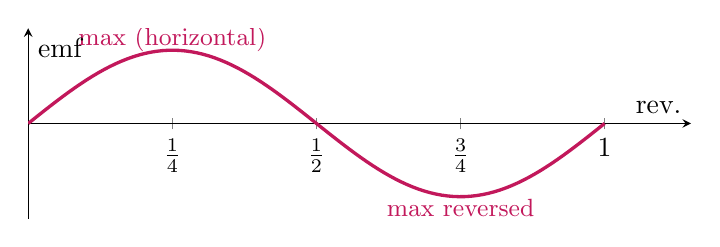
\begin{tikzpicture}
\begin{axis}[width=10cm,height=4cm,axis lines=middle,xmin=0,xmax=1.15,ymin=-1.3,ymax=1.3,
  xtick={0.25,0.5,0.75,1},xticklabels={$\frac14$,$\frac12$,$\frac34$,1},ytick=\empty,xlabel={rev.},ylabel={emf}]
\addplot[anscol,very thick,domain=0:1,samples=100] {sin(deg(2*pi*x))};
\node[font=\small,anscol] at (axis cs:0.25,1.15) {max (horizontal)};
\node[font=\small,anscol] at (axis cs:0.75,-1.15) {max reversed};
\end{axis}\end{tikzpicture}\\\small Zero at 0, $\frac12$, 1 rotation (coil vertical); maximum at $\frac14$ and $\frac34$ (coil horizontal).}
\item Why does the emf vary from zero to maximum during a rotation? \mk{2M}
\answer[3]{The emf depends on how fast the flux through the coil changes. When the coil is vertical (plane $\perp$ field) the flux is maximum but changing slowest, so the emf is zero. When it is horizontal (plane $\parallel$ field) the flux is changing fastest, so the emf is maximum.}
\item How is an AC generator converted into a DC generator? \mk{2M}
\answer[3]{Replace the two full slip rings by two half (split) rings. After every half rotation the ends of the coil change brushes, so the current in the external circuit always flows in the same direction (DC).}
\end{enumerate}

\exhead{D}{Textbook application}{\tb\ \asbadge{AS7}\ \badge{2M}}
Give a few applications of Faraday's law of induction in daily life. \mk{2M}
\answer[4]{Electric generators in power stations; metal detectors at security checks; tape recorder heads; induction stoves; ATM/credit card readers; transformers; bicycle dynamo.}

\selfcheck{25}{
\item explain four applications of induction
\item explain levitation with AC and why DC fails
\item explain the AC generator, its emf graph and the DC version}

% =====================================================================
\clearpage
\section*{\sffamily\color{ecblue}One-mark rapid fire}
{\small Answer in one word or one line. Target \textbf{8 minutes} for 25 questions.}\hfill Time taken: \rule{1.6cm}{0.3pt}\qquad Score: \rule{1cm}{0.3pt} / 25
\vspace{4pt}
\renewcommand{\arraystretch}{1.55}
\begin{multicols}{2}
\begin{enumerate}[itemsep=5pt]
\item Discovered the magnetic effect of current? \blank[2cm]{Oersted}
\item Unit of magnetic flux? \blank[2cm]{weber}
\item Unit of flux density? \blank[2cm]{tesla}
\item 1 T in N, A, m? \blank[2cm]{N/(A m)}
\item $\Phi$ for a plane $\parallel B$? \blank[2cm]{zero}
\item Field lines of a straight wire? \blank[2cm]{circles}
\item Current $\odot$: field lines are? \blank[2cm]{anticlockwise}
\item Rule for field of a wire? \blank[2cm]{thumb rule}
\item Anticlockwise current face is? \blank[2cm]{N pole}
\item Coil that acts like a bar magnet? \blank[2cm]{solenoid}
\item Force on a charge moving $\parallel B$? \blank[2cm]{zero}
\item Formula for force on a charge? \blank[2cm]{$qvB\sin\theta$}
\item Radius of path of a charge? \blank[2cm]{$mv/Bq$}
\item Force on a current $\perp B$? \blank[2cm]{$ILB$}
\item Motor converts? \blank[2cm]{elec.\ $\to$ mech.}
\item Reverses current in a motor? \blank[2cm]{split rings}
\item Faraday's law formula? \blank[2cm]{$\Delta\Phi/\Delta t$}
\item Law giving induced current direction? \blank[2cm]{Lenz's law}
\item Lenz's law is based on? \blank[2cm]{energy cons.}
\item Motional emf? \blank[2cm]{$Blv$}
\item Emf when coil plane $\perp B$ (generator)? \blank[2cm]{zero}
\item Rings in an AC generator? \blank[2cm]{slip rings}
\item Generator converts? \blank[2cm]{mech.\ $\to$ elec.}
\item Stove using induction? \blank[2cm]{induction stove}
\item Current reversing periodically? \blank[2cm]{AC}
\end{enumerate}
\end{multicols}

% =====================================================================
\clearpage
\section*{\sffamily\color{ecblue}Score boosters}
\subsection*{\sffamily Anatomy of a full-marks 4-mark answer}
{\small Example question: \emph{Explain the working of an electric motor.}}\par\vspace{2pt}
\renewcommand{\arraystretch}{1.5}
\begin{tabularx}{\linewidth}{>{\bfseries\sffamily\small}p{2.6cm}X>{\small}p{2.7cm}}
\toprule
\rowcolor{ecteal!15}Part & \textbf{What to write} & \textbf{Why it matters}\\
\midrule
1. Principle & A current-carrying coil in a field experiences a force ($F=ILB$). & Scores the concept mark.\\
2. Diagram & Coil ABCD between N and S, split rings, brushes, battery; arrows for current. & Diagrams carry marks.\\
3. Forces & AB and CD: equal, opposite forces $\Rightarrow$ couple $\Rightarrow$ rotation. & Shows you know why.\\
4. Commutator & Split rings reverse current every half turn $\Rightarrow$ continuous rotation. & Key idea examiners look for.\\
5. Energy & Electrical energy $\to$ mechanical energy. & Closes the answer.\\
\bottomrule
\end{tabularx}

\subsection*{\sffamily Keywords the examiner looks for}
\renewcommand{\arraystretch}{1.35}
\begin{tabularx}{\linewidth}{>{\bfseries\small}p{3.8cm}>{\small}X}
\toprule
Oersted & compass deflects $\cdot$ current produces field\\
Field lines & tangent gives direction $\cdot$ crowded = strong $\cdot$ closed loops\\
Straight wire & concentric circles $\cdot$ right hand thumb rule\\
Force & $qvB\sin\theta$ $\cdot$ $ILB\sin\theta$ $\cdot$ zero when parallel $\cdot$ right hand rule\\
Motor & couple $\cdot$ split rings $\cdot$ brushes $\cdot$ electrical to mechanical\\
Faraday & change of flux $\cdot$ rate of change $\cdot$ induced emf\\
Lenz & opposes the change $\cdot$ conservation of energy\\
Generator & rotating coil $\cdot$ slip rings $\cdot$ zero/maximum emf $\cdot$ mechanical to electrical\\
\bottomrule
\end{tabularx}

\begin{examtip}[Mistakes that cost marks]
\begin{multicols}{2}\small
\begin{itemize}[leftmargin=4mm,itemsep=1pt]
\item Field lines without arrows.
\item $\theta$ measured from the plane, not the normal, in $\Phi=BA\cos\theta$.
\item Forgetting $F=0$ when parallel to $B$.
\item Not reversing the force for an electron.
\item Using cm or cm$^2$ without converting.
\item Forgetting $N$ in $\varepsilon=N\Delta\Phi_0/\Delta t$.
\item Slip rings in a motor (it has split rings).
\item No energy argument in Lenz's law.
\end{itemize}
\end{multicols}
\end{examtip}

\subsection*{\sffamily Formula sheet \normalfont\small(cover the right column and test yourself)}
\renewcommand{\arraystretch}{1.7}
\begin{tabularx}{\linewidth}{>{\bfseries\small}p{5.3cm}X}
\toprule
\rowcolor{ecred}\textcolor{white}{Quantity} & \textcolor{white}{\textbf{Formula / unit}}\\
\midrule
Flux density & $B=\dfrac{\Phi}{A}$ \quad tesla = Wb/m$^2$\\
Flux & $\Phi=BA\cos\theta$ \quad weber\\
Force on a charge & $F=qvB\sin\theta$\\
Circular motion & $r=\dfrac{mv}{Bq}$,\quad $T=\dfrac{2\pi m}{Bq}$\\
Force on a current & $F=ILB\sin\theta$\\
Faraday's law & $\varepsilon=\dfrac{\Delta\Phi}{\Delta t}$;\quad $\varepsilon=N\dfrac{\Delta\Phi_0}{\Delta t}$\\
Motional emf & $\varepsilon=Blv$\\
\bottomrule
\end{tabularx}

\subsection*{\sffamily Diagram practice tracker}
{\small Draw each diagram three times on separate days. Tick when you can draw it from memory in under 4 minutes.}\par
\renewcommand{\arraystretch}{1.4}
\begin{tabularx}{\linewidth}{X c c c}
\toprule
\textbf{Diagram} & \textbf{Try 1} & \textbf{Try 2} & \textbf{Try 3}\\
\midrule
Field lines of a bar magnet & \tick & \tick & \tick\\
Field of a straight wire ($\odot$ and $\otimes$) & \tick & \tick & \tick\\
Field of a solenoid with N and S & \tick & \tick & \tick\\
Right hand rule for force & \tick & \tick & \tick\\
Electric motor with split rings & \tick & \tick & \tick\\
Faraday's activity (magnet, coil, galvanometer) & \tick & \tick & \tick\\
AC generator and emf graph & \tick & \tick & \tick\\
\bottomrule
\end{tabularx}

% =====================================================================
\clearpage
\section*{\sffamily\color{ecblue}Chapter test}
\begin{tcolorbox}[wbox,colback=ecblue!5,colframe=ecblue]
\sffamily\small\textbf{Time: 1 hour 30 minutes \hfill Maximum marks: 40}\\[2pt]
\rmfamily Section I: 6 questions $\times$ 1 mark. Section II: 5 questions $\times$ 2 marks. Section III: 4 questions $\times$ 4 marks, each with an internal choice. Section IV: 8 multiple choice questions $\times$ 1 mark.
\end{tcolorbox}

\exhead{Section I}{}{\badge{6 $\times$ 1 = 6}}
\begin{enumerate}
\item What is the SI unit of magnetic flux density? \answer[1]{Tesla (Wb/m$^2$).}
\item State Lenz's law. \answer[1]{The induced current opposes the change in flux producing it.}
\item What is the force on a current-carrying wire kept parallel to a magnetic field? \answer[1]{Zero.}
\item Which device converts mechanical energy into electrical energy? \answer[1]{Generator.}
\item Write the formula for motional emf. \answer[1]{$\varepsilon=Blv$.}
\item Name the rule used to find the direction of the field around a straight wire. \answer[1]{Right hand thumb rule.}
\end{enumerate}

\exhead{Section II}{}{\badge{5 $\times$ 2 = 10}}
\begin{enumerate}[resume]
\item Why does a TV picture get distorted when a magnet is brought near it? \answer[3]{The picture is made by moving electrons; the magnet's field exerts a force on them and deflects them.}
\item A 0.5 m wire carries 2 A perpendicular to a field of 0.4 T. Find the force. \answer[2]{$F=ILB=2\times0.5\times0.4=0.4$ N.}
\item A coil of 50 turns has its flux per turn changed by 0.02 Wb in 0.1 s. Find the induced emf. \answer[2]{$\varepsilon=\frac{50\times0.02}{0.1}=10$ V.}
\item Are magnetic field lines closed? Explain. \answer[3]{Yes: circles round a wire; for a solenoid/magnet the lines go N $\to$ S outside and S $\to$ N inside.}
\item A coil and a magnet move together in the same direction at the same speed. Is a current induced? Why? \answer[3]{No: no relative motion, so no change of flux.}
\end{enumerate}

\exhead{Section III}{}{\badge{4 $\times$ 4 = 16}}
\begin{enumerate}[resume]
\item Explain with two activities that a current-carrying wire produces a magnetic field.\\
\textbf{OR}\quad Describe an activity to show that a current-carrying wire experiences a force in a magnetic field.
\answer[8]{See Unit 3, Exercise D or Unit 5, Exercise E.}
\item Derive $F=ILB$ for a straight wire in a magnetic field.\\
\textbf{OR}\quad Derive $r=\dfrac{mv}{Bq}$ and $T=\dfrac{2\pi m}{Bq}$ for a charge moving perpendicular to a field.
\answer[8]{See Unit 5, Exercise A or Unit 4, Exercise B.}
\item Derive $\varepsilon=Blv$ using conservation of energy.\\
\textbf{OR}\quad State Faraday's law and explain it with an activity.
\answer[8]{See Unit 6, Exercise C or Exercise F1.}
\item Explain the working of an electric motor with a diagram.\\
\textbf{OR}\quad Explain the working of an AC generator with the graph of emf for one rotation.
\answer[8]{See the anatomy table in Score boosters (motor) or Unit 7, Exercise C.}
\end{enumerate}

\exhead{Section IV}{}{\badge{8 $\times$ 1 = 8}}
\begin{enumerate}[resume]
\mcq{Which converts electrical energy into mechanical energy?}{motor}{battery}{generator}{switch}{A}
\mcq{The force on a wire perpendicular to a uniform field is}{0}{$ILB$}{$2ILB$}{$ILB/2$}{B}
\mcq{One tesla is equal to}{N/C}{N/(A m)}{A/m}{N/(A s)}{B}
\mcq{Unit of magnetic flux is}{dyne}{oersted}{gauss}{weber}{D}
\mcq{No force acts on a current-carrying conductor kept}{parallel to the field}{perpendicular to the field}{in the field}{away from the field}{A}
\mcq{Current flows anticlockwise in a coil as you see it. The face towards you is}{S pole}{N pole}{neither}{both}{B}
\mcq{In an AC generator the emf is maximum when the plane of the coil is}{perpendicular to $B$}{parallel to $B$}{at $45^\circ$}{at rest}{B}
\mcq{The time period of a charge moving in a circle in a uniform field depends on}{its speed}{the radius}{$m$, $q$ and $B$}{none}{C}
\end{enumerate}

\vspace{6pt}
\begin{tcolorbox}[wbox,colback=ecgold!10,colframe=ecorange,title={\faChartLine\ My test result}]
\renewcommand{\arraystretch}{1.6}
\begin{tabularx}{\linewidth}{X c c c c c}
Section & I & II & III & IV & \textbf{Total}\\
Marks & \rule{0.9cm}{0.3pt}\,/6 & \rule{0.9cm}{0.3pt}\,/10 & \rule{0.9cm}{0.3pt}\,/16 & \rule{0.9cm}{0.3pt}\,/8 & \rule{0.9cm}{0.3pt}\,/40\\
\end{tabularx}
\end{tcolorbox}

% =====================================================================
\clearpage
\section*{\sffamily\color{ecblue}Mistake log}
{\small Write every question you got wrong. Redo it after one week without looking at the answer.}\par\vspace{4pt}
\renewcommand{\arraystretch}{2.5}
\begin{tabularx}{\linewidth}{|p{1.4cm}|X|X|c|}
\hline
\rowcolor{ecblue!12}\textbf{Unit / Q} & \textbf{What I wrote} & \textbf{The correct idea} & \textbf{Redone}\\\hline
\logrow\logrow\logrow\logrow\logrow\logrow\logrow\logrow\logrow\logrow\logrow\logrow\logrow\logrow
\end{tabularx}

\end{document}
"
\documentclass[11pt,a4paper]{article}
\usepackage[a4paper,margin=17mm,top=20mm,bottom=20mm,headsep=6mm]{geometry}
\usepackage[T1]{fontenc}
\usepackage{newtxtext,newtxmath}
\usepackage{amsmath}
\usepackage{graphicx}
\usepackage{tikz}
\usetikzlibrary{arrows.meta,calc,decorations.markings}
\usepackage[american]{circuitikz}
\usepackage{pgfplots}
\pgfplotsset{compat=1.18}
\usepackage[most]{tcolorbox}
\usepackage{booktabs,array,tabularx,multicol}
\usepackage[table]{xcolor}
\usepackage{enumitem}
\usepackage{fontawesome5}
\usepackage[normalem]{ulem}
\usepackage{fancyhdr}
\usepackage{xparse}
\graphicspath{{figures/}}

% ---------------- edition switch ----------------
\newif\ifanswers
\ifdefined\withanswers\answerstrue\fi

% ---------------- colours (same as the classroom deck) ----------------
\definecolor{ecblue}{HTML}{1F4E9A}
\definecolor{ecteal}{HTML}{0E8C8C}
\definecolor{ecorange}{HTML}{E8710A}
\definecolor{ecred}{HTML}{C62828}
\definecolor{ecgreen}{HTML}{2E7D32}
\definecolor{ecpurple}{HTML}{6A1B9A}
\definecolor{ecgold}{HTML}{F9A825}
\definecolor{ecnavy}{HTML}{0D2B5E}
\definecolor{anscol}{HTML}{C2185B}
\definecolor{rulecol}{HTML}{9AA7BD}

\setlength{\parindent}{0pt}
\setlength{\parskip}{3pt}
\setlist{itemsep=3pt,topsep=3pt}
\setlist[enumerate,1]{label=\textbf{\arabic*.},leftmargin=7mm}

% ---------------- header / footer ----------------
\pagestyle{fancy}
\fancyhf{}
\renewcommand{\headrulewidth}{0.4pt}
\fancyhead[L]{\small\sffamily\color{ecblue}Magnetic Effects of Electric Current \;$\cdot$\; Workbook}
\fancyhead[R]{\small\sffamily\ifanswers\textcolor{anscol}{\textbf{ANSWER KEY}}\;$\cdot$\;\fi Class X Physical Science}
\fancyfoot[C]{\small\sffamily\thepage}
\fancyfoot[R]{\ifanswers\else\scriptsize\sffamily\color{gray}Name: \rule{3.5cm}{0.3pt}\fi}

% ---------------- building blocks ----------------
\newcommand{\badge}[1]{\tikz[baseline=(b.base)]\node[fill=ecgold,text=black,rounded corners=2.5pt,
  inner sep=2pt,font=\sffamily\scriptsize\bfseries](b){#1};}
\newcommand{\asbadge}[1]{\tikz[baseline=(b.base)]\node[draw=ecteal,text=ecteal,rounded corners=2.5pt,
  inner sep=1.6pt,font=\sffamily\scriptsize\bfseries](b){#1};}
\newcommand{\tb}{\tikz[baseline=(b.base)]\node[fill=ecblue,text=white,rounded corners=2.5pt,
  inner sep=1.8pt,font=\sffamily\scriptsize\bfseries](b){Textbook};}
\newcommand{\imp}[1]{\textcolor{ecred}{\textbf{#1}}}
\newcommand{\key}[1]{\textcolor{ecblue}{\textbf{#1}}}
\newcommand{\mk}[1]{\hfill\badge{#1}}
\newcommand{\tick}{\faSquare[regular]}
\newcommand{\logrow}{ & & & \tick\\\hline}
\newcommand{\bx}[1]{[\,\makebox[1em]{\ifanswers\textcolor{anscol}{\textbf{#1}}\fi}\,]}

% blank for a word or phrase
\newcommand{\blank}[2][2.8cm]{\ifanswers\leavevmode{\color{anscol}\bfseries\uline{#2}}\else\rule[-2pt]{#1}{0.5pt}\fi}
% blank inside mathematics
\newcommand{\mblank}[2][1.8cm]{\ifanswers\leavevmode{\color{anscol}\ensuremath{#2}}\else\ensuremath{\underline{\hspace{#1}}}\fi}
% ruled writing lines
\newcommand{\writelines}[1]{\par\foreach\n in {1,...,#1}{\vspace*{7.2mm}\noindent{\color{rulecol}\rule{\linewidth}{0.4pt}}\par}\vspace{1mm}}
% answer box in key, ruled lines in student edition
\newtcolorbox{anskey}{enhanced,breakable,colback=anscol!4,colframe=anscol!70,boxrule=0.5pt,arc=1.5mm,
  left=5pt,right=5pt,top=3pt,bottom=3pt,fontupper=\small,before skip=4pt,after skip=6pt}
\NewDocumentCommand{\answer}{O{3} +m}{\ifanswers\begin{anskey}#2\end{anskey}\else\writelines{#1}\fi}
% drawing space: grid box for students, model diagram in key
\NewDocumentCommand{\drawbox}{m +m}{\ifanswers\begin{anskey}\centering #2\end{anskey}\else
  \begin{tcolorbox}[enhanced,height=#1,colback=white,colframe=rulecol,boxrule=0.5pt,arc=1mm,
    interior code={\fill[white] (interior.south west) rectangle (interior.north east);
    \draw[step=5mm,gray!18] (interior.south west) grid (interior.north east);}]
  \end{tcolorbox}\fi}
% MCQ: question, four options, correct letter
\NewDocumentCommand{\mcq}{m m m m m m}{\item #1\hfill\textbf{[\,\makebox[1.2em]{\ifanswers\textcolor{anscol}{#6}\fi}\,]}\\[1pt]
  \begin{tabular}{@{}p{0.47\linewidth}p{0.47\linewidth}@{}}A) #2 & B) #3\\ C) #4 & D) #5\end{tabular}}
% true/false
\NewDocumentCommand{\tf}{m m m}{\item #1\hfill\textbf{[\,\makebox[1.2em]{\ifanswers\textcolor{anscol}{#2}\fi}\,]}
  \ifanswers\ifx&#3&\else\\{\small\textcolor{anscol}{Correct: #3}}\fi\fi}

% boxes
\tcbset{wbox/.style={enhanced,breakable,boxrule=0.8pt,arc=2mm,left=6pt,right=6pt,top=3pt,bottom=4pt,
  fonttitle=\sffamily\bfseries\small,before skip=6pt,after skip=6pt}}
\newtcolorbox{recall}{wbox,colback=ecblue!5,colframe=ecblue,title={\faBolt\ Recall in 60 seconds}}
\newtcolorbox{examtip}[1][Exam tip]{wbox,colback=ecgold!12,colframe=ecorange,title={\faStar\ #1}}
\newtcolorbox{worked}[1][Worked example]{wbox,colback=ecgreen!5,colframe=ecgreen,title={\faCheckCircle\ #1}}
\newtcolorbox{hots}[1][Think deeper (HOTS)]{wbox,colback=ecpurple!5,colframe=ecpurple,title={\faBrain\ #1}}

% colour strip
\newcommand{\ecstrip}[2]{\tikz{\foreach \c [count=\i] in {ecnavy,ecblue,ecteal,ecgreen,ecgold,ecorange,ecred}
  \fill[\c] ({(\i-1)*#1/7},0) rectangle ++(#1/7,#2);}}

% unit banner
\newcounter{unit}
\NewDocumentCommand{\unit}{m m}{\clearpage\stepcounter{unit}%
  \begin{tcolorbox}[enhanced,colback=ecblue,colframe=ecblue,arc=0mm,boxrule=0pt,left=8pt,top=6pt,bottom=6pt,
    before skip=0pt,after skip=0pt]
  \sffamily\color{white}{\small UNIT \theunit}\\[1pt]{\LARGE\bfseries #1}\hfill{#2}
  \end{tcolorbox}\par\nointerlineskip
  \ecstrip{\linewidth}{0.14}\par\vspace{4pt}}
% exercise heading
\newcommand{\exhead}[3]{\par\vspace{8pt}{\sffamily\bfseries\color{ecblue}\large #1\quad #2}\hfill{#3}\par
  \vspace{-4pt}{\color{ecblue!40}\rule{\linewidth}{0.6pt}}\par\vspace{2pt}}
% end-of-unit self check
\NewDocumentCommand{\selfcheck}{m +m}{\par\vspace{8pt}\begin{tcolorbox}[wbox,colback=ecteal!6,colframe=ecteal,
  title={\faClipboardCheck\ Self check}]
  \begin{minipage}[t]{0.68\linewidth}\small\textbf{I can \dots}\\[-2pt]
  \begin{itemize}[label=\tick,leftmargin=6mm,itemsep=0pt]#2\end{itemize}\end{minipage}\hfill
  \begin{minipage}[t]{0.28\linewidth}\centering\small\textbf{My score}\\[4pt]
  {\Large\rule{1.2cm}{0.4pt} / #1}\\[6pt]\scriptsize Redo every question you got wrong on the \textbf{Mistake log} page.\end{minipage}
  \end{tcolorbox}}

\ctikzset{bipoles/length=1.0cm}
\definecolor{fieldc}{HTML}{0097A7}
\tikzset{cur/.style={-{Stealth[length=5pt]},ecred,thick},acur/.style={-{Stealth[length=5pt]},anscol,thick},
  fl/.style={fieldc,thick,postaction={decorate},decoration={markings,mark=at position #1 with {\arrow{Stealth[length=5pt]}}}},fl/.default=0.5,
  afl/.style={anscol,thick,postaction={decorate},decoration={markings,mark=at position #1 with {\arrow{Stealth[length=5pt]}}}},afl/.default=0.5,
  flab/.style={font=\sffamily\small,inner sep=1.5pt},fptr/.style={-{Stealth[length=4pt]},ecred,thick}}
\newcommand{\outpage}[2][0.18]{\draw[thick,fill=white] #2 circle (#1); \fill #2 circle (#1*0.28);}
\newcommand{\inpage}[2][0.18]{\draw[thick,fill=white] #2 circle (#1);
  \draw[thick] ($#2+(-#1*0.6,-#1*0.6)$) -- ($#2+(#1*0.6,#1*0.6)$) ($#2+(-#1*0.6,#1*0.6)$) -- ($#2+(#1*0.6,-#1*0.6)$);}
\newcommand{\figlab}[3]{\begin{tikzpicture}
  \node[inner sep=0,anchor=south west] (im) at (0,0) {\includegraphics[#2]{#1}};
  \begin{scope}[x={(im.south east)},y={(im.north west)}]#3\end{scope}\end{tikzpicture}}

\begin{document}

% =====================================================================
% COVER
% =====================================================================
\thispagestyle{empty}
\begin{tikzpicture}[remember picture,overlay]
  \fill[ecblue] (current page.north west) rectangle ([yshift=-9cm]current page.north east);
  \foreach \c [count=\i] in {ecnavy,ecblue,ecteal,ecgreen,ecgold,ecorange,ecred}
    \fill[\c] ([yshift=-9cm-(\i-1)*0.18cm]current page.north west) rectangle
              ([yshift=-9cm-\i*0.18cm]current page.north east);
  \node[white,font=\sffamily\large\bfseries,anchor=west] at ([xshift=1.8cm,yshift=-2.0cm]current page.north west)
     {CLASS X \;$\cdot$\; PHYSICAL SCIENCE \;$\cdot$\; CHAPTER 10};
  \node[white,font=\sffamily\fontsize{36}{40}\selectfont\bfseries,anchor=west] at ([xshift=1.7cm,yshift=-3.8cm]current page.north west) {Magnetic Effects of};
  \node[white,font=\sffamily\fontsize{36}{40}\selectfont\bfseries,anchor=west] at ([xshift=1.7cm,yshift=-5.4cm]current page.north west) {Electric Current};
  \node[ecgold,font=\sffamily\LARGE\bfseries,anchor=west] at ([xshift=1.8cm,yshift=-7.3cm]current page.north west)
     {Student Workbook\ifanswers\ \textcolor{white}{--} \textcolor{white}{Answer Key}\fi};
  \node[anchor=north east] at ([xshift=-1.2cm,yshift=-10.8cm]current page.north east) {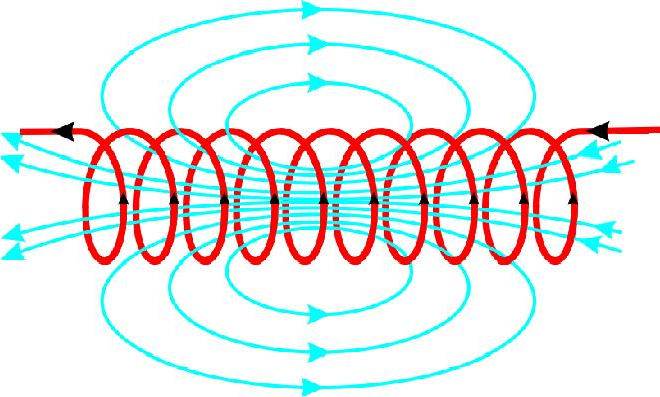
\includegraphics[height=3.8cm]{solenoid_field.png}};
  \node[anchor=north west,text width=9.4cm,font=\sffamily,align=left] at ([xshift=1.8cm,yshift=-10.8cm]current page.north west) {%
    {\large\bfseries Practise the way the exam asks.}\\[6pt]
    \small Every topic of the chapter, turned into questions you answer in this book:
    fill in the blanks, label and draw field lines, apply the hand rules, complete the
    derivation, solve the numerical, explain the reason. Each unit ends with a self check,
    and the book ends with a full 40-mark chapter test.\\[10pt]
    \faStar\ Marks badges: \badge{1M} \badge{2M} \badge{4M}\\[4pt]
    \faStar\ Academic standards: \asbadge{AS1} concept \asbadge{AS3} experiment \asbadge{AS5} diagram \asbadge{AS7} application\\[4pt]
    \faStar\ \tb\ marks every question from \emph{Improve your learning}};
  \node[anchor=south west,font=\sffamily] at ([xshift=1.8cm,yshift=2.2cm]current page.south west) {%
    \renewcommand{\arraystretch}{2.1}
    \begin{tabular}{@{}l@{\quad}p{8.5cm}@{}}
    \textbf{Name} & \hrulefill\\
    \textbf{Class / Section} & \hrulefill\\
    \textbf{Roll No.} & \hrulefill\\
    \textbf{School} & \hrulefill\\
    \end{tabular}};
\end{tikzpicture}
\null\clearpage

% =====================================================================
\section*{\sffamily\color{ecblue}How to use this workbook}
\begin{enumerate}[label=\textcolor{ecorange}{\faArrowRight},leftmargin=6mm]
\item Read the \textbf{Recall in 60 seconds} box first. If a point feels new, go back to the textbook page before you start.
\item Answer in the book, in pen. Do the questions \textbf{without} looking at the textbook, then check.
\item Numericals: \emph{formula $\rightarrow$ values in SI units (m, m$^2$, A, T) $\rightarrow$ answer with unit}.
\item Field-line diagrams: draw in pencil, put \textbf{arrows on every line}, mark N and S, $\odot$ and $\otimes$.
\item For every direction question, write which \textbf{rule} you used (thumb rule, right hand rule, Lenz's law).
\item Fill in the \textbf{Self check} after each unit; copy mistakes into the \textbf{Mistake log}.
\end{enumerate}

\subsection*{\sffamily\color{ecblue}What the exam asks from this chapter}
\renewcommand{\arraystretch}{1.35}
\begin{tabularx}{\linewidth}{>{\bfseries\sffamily}p{1.6cm}X}
\toprule
\rowcolor{ecblue}\textcolor{white}{Marks} & \textcolor{white}{\textbf{\sffamily Typical questions}}\\
\midrule
1 mark & Units (weber, tesla), one-line laws, energy change in motor/generator, force when parallel to $B$, MCQs.\\
2 marks & Direction of current/field/force from a figure, pole of a coil, TV distortion, closed field lines, short numericals on $B=\Phi/A$, $F=ILB$, $\varepsilon=Blv$, $\varepsilon=N\Delta\Phi/\Delta t$.\\
4 marks & Activities: current produces a field; force on a wire; Faraday's law. Working of motor and generators. Derivation of $\varepsilon=Blv$, $F=ILB$, $r=mv/Bq$. Lenz's law with energy argument. Levitation.\\
Diagrams & Field lines of bar magnet, straight wire, solenoid; right hand rules; coil in a field; motor; Faraday's activity; AC generator and emf graph.\\
\bottomrule
\end{tabularx}

\subsection*{\sffamily\color{ecblue}My progress tracker}
\renewcommand{\arraystretch}{1.55}
\begin{tabularx}{\linewidth}{>{\sffamily}l X c c c}
\toprule
\rowcolor{ecteal!15}\textbf{Unit} & \textbf{Topic} & \textbf{Score} & \textbf{Confidence} & \textbf{Revised on}\\
\midrule
1 & Oersted, magnetic field and field lines & \rule{1.3cm}{0.3pt} & \tick\,\tick\,\tick & \rule{1.6cm}{0.3pt}\\
2 & Magnetic flux and flux density & \rule{1.3cm}{0.3pt} & \tick\,\tick\,\tick & \rule{1.6cm}{0.3pt}\\
3 & Fields of a wire, coil and solenoid & \rule{1.3cm}{0.3pt} & \tick\,\tick\,\tick & \rule{1.6cm}{0.3pt}\\
4 & Force on a moving charge & \rule{1.3cm}{0.3pt} & \tick\,\tick\,\tick & \rule{1.6cm}{0.3pt}\\
5 & Force on a current; electric motor & \rule{1.3cm}{0.3pt} & \tick\,\tick\,\tick & \rule{1.6cm}{0.3pt}\\
6 & Induction: Faraday, Lenz, motional emf & \rule{1.3cm}{0.3pt} & \tick\,\tick\,\tick & \rule{1.6cm}{0.3pt}\\
7 & Applications, levitation, generators & \rule{1.3cm}{0.3pt} & \tick\,\tick\,\tick & \rule{1.6cm}{0.3pt}\\
-- & One-mark rapid fire & \rule{1.3cm}{0.3pt} & \tick\,\tick\,\tick & \rule{1.6cm}{0.3pt}\\
-- & Chapter test (40 marks) & \rule{1.3cm}{0.3pt} & \tick\,\tick\,\tick & \rule{1.6cm}{0.3pt}\\
\bottomrule
\end{tabularx}
{\small Confidence: tick one box for ``shaky'', two for ``fine'', three for ``I can teach it''.}

% =====================================================================
\unit{Magnetic field and field lines}{\badge{1M}\ \badge{2M}\ \badge{4M}}
% =====================================================================
\begin{recall}
\begin{itemize}[leftmargin=5mm,itemsep=0pt]
\item \key{Oersted (1820)}: a compass needle under a wire deflects when current flows $\Rightarrow$ a current produces a magnetic field.
\item A \key{magnetic field} is the region around a magnet where its force acts without contact. It has \textbf{strength} and \textbf{direction} and is three-dimensional.
\item \key{Field lines} are imaginary; the \textbf{tangent} gives the direction; crowded lines = strong field. Outside a magnet they go N $\to$ S. Uniform field: parallel, equally spaced lines.
\end{itemize}
\end{recall}

\exhead{A}{Fill in the blanks}{\asbadge{AS1}\ \badge{1M}}
\begin{enumerate}
\item The scientist who first showed that a current deflects a compass needle was \blank{Oersted}.
\item The direction of the field at a point is given by the \blank{tangent} to the field line at that point.
\item Field lines are \blank{crowded} near the poles, where the field is \blank{strong}.
\item A field whose strength and direction are the same everywhere is called a \blank{uniform} field.
\item Outside a bar magnet field lines go from \blank[1.5cm]{N} to \blank[1.5cm]{S}.
\end{enumerate}

\exhead{B}{True or false}{\asbadge{AS1}\ \badge{1M}}
{\small Write T or F. If false, correct it on the line below.}
\begin{enumerate}
\tf{Field lines of a magnet can cross each other.}{F}{They never cross; at a crossing the field would have two directions, which is impossible.}
\ifanswers\else\writelines{1}\fi
\tf{The magnetic field of a bar magnet exists only in the plane of the paper.}{F}{It is three-dimensional; it surrounds the magnet in all directions.}
\ifanswers\else\writelines{1}\fi
\tf{Far from a magnet a compass needle points almost north--south.}{T}{}
\ifanswers\else\writelines{1}\fi
\end{enumerate}

\exhead{C}{Label the Oersted apparatus}{\asbadge{AS5}\ \badge{2M}}
\begin{center}
\figlab{oersted_setup.png}{width=0.62\linewidth}{
\draw[fptr] (0.18,1.12) node[flab,anchor=south]{(a) \blank[2.3cm]{copper wire}} -- (0.36,0.82);
\draw[fptr] (0.85,1.12) node[flab,anchor=south]{(b) \blank[2.3cm]{battery}} -- (0.66,0.78);
\draw[fptr] (0.20,0.05) node[flab,anchor=north]{(c) \blank[2.3cm]{compass}} -- (0.40,0.60);
\draw[fptr] (0.72,0.05) node[flab,anchor=north]{(d) \blank[2.3cm]{key}} -- (0.54,0.40);}
\end{center}
\vspace{6pt}
\begin{enumerate}
\item What happens to the needle when the key is closed? What does it prove? \mk{2M}
\answer[3]{The needle deflects. When the key is opened it returns to the north--south direction. This proves that a current-carrying wire produces a magnetic field around it: electricity and magnetism are related.}
\end{enumerate}

\exhead{D}{Draw field lines}{\asbadge{AS5}\ \badge{2M}}
Draw at least six field lines of the bar magnet below, with arrows. \mk{2M}
\begin{center}
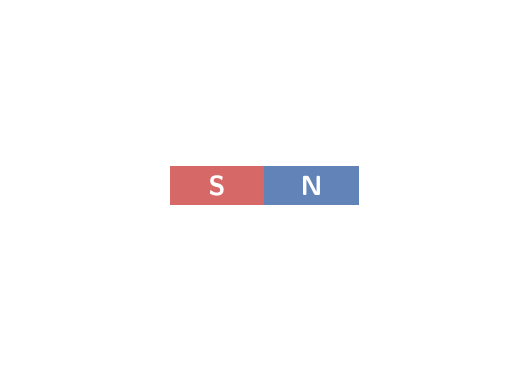
\begin{tikzpicture}
\fill[ecred!70] (-1.2,-0.25) rectangle (0,0.25); \fill[ecblue!70] (0,-0.25) rectangle (1.2,0.25);
\node[white,font=\sffamily\bfseries] at (-0.6,0) {S}; \node[white,font=\sffamily\bfseries] at (0.6,0) {N};
\ifanswers
\foreach \h in {0.8,1.4,2.1}{
  \draw[afl=0.5] (1.2,0.1) .. controls (2.5,\h) and (-2.5,\h) .. (-1.2,0.1);
  \draw[afl=0.5] (1.2,-0.1) .. controls (2.5,-\h) and (-2.5,-\h) .. (-1.2,-0.1);}
\draw[afl=0.5] (1.2,0) -- (3,0); \draw[afl=0.5] (-3,0) -- (-1.2,0);
\else
\draw[white] (-3,-2) rectangle (3,2);
\fi
\end{tikzpicture}
\end{center}

\exhead{E}{Short answers}{\tb\ \asbadge{AS1}\ \badge{2M}}
\begin{enumerate}
\item Are magnetic field lines closed? Explain. \mk{2M}
\answer[4]{Yes. Around a straight wire they are complete circles. For a solenoid (and a bar magnet) the lines outside go from N to S and continue inside from S to N, so every line is a closed loop.}
\item How can you find the strength and the direction of a magnetic field using field lines? \mk{2M}
\answer[3]{Direction: the tangent to the field line at the point (the way a compass needle points). Strength: how close the lines are; crowded lines mean a strong field, widely spaced lines a weak field.}
\end{enumerate}

\selfcheck{19}{
\item describe Oersted's experiment and its conclusion
\item state the properties of field lines
\item draw the field lines of a bar magnet with arrows}

% =====================================================================
\unit{Magnetic flux and flux density}{\badge{1M}\ \badge{2M}}
% =====================================================================
\begin{recall}
\begin{itemize}[leftmargin=5mm,itemsep=0pt]
\item \key{Magnetic flux} $\Phi$: number of field lines through a plane held perpendicular to the field. Unit \imp{weber (Wb)}.
\item \key{Flux density} $B=\dfrac{\Phi}{A}$ (area perpendicular to the field). Unit \imp{Wb/m$^2$ = tesla (T)}.
\item Plane tilted so its normal makes $\theta$ with $B$: effective area $A\cos\theta$, so \imp{$\Phi=BA\cos\theta$}. Plane parallel to $B$: $\Phi=0$.
\end{itemize}
\end{recall}

\exhead{A}{Fill in the blanks}{\asbadge{AS1}\ \badge{1M}}
\begin{enumerate}
\item The SI unit of magnetic flux is the \blank{weber}.
\item The SI unit of magnetic flux density is the \blank{tesla}, which equals \blank{Wb/m$^2$}.
\item Magnetic flux density is also called magnetic \blank{induction}.
\item The flux through a plane held parallel to the field is \blank[1.5cm]{zero}.
\end{enumerate}

\exhead{B}{Complete the derivation of $\Phi=BA\cos\theta$}{\asbadge{AS1}\ \badge{2M}}
\noindent
\begin{minipage}[c]{0.38\linewidth}\centering
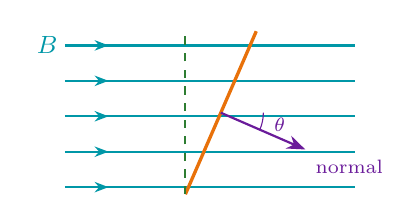
\begin{tikzpicture}[scale=0.9]
\foreach \y in {0.2,0.7,1.2,1.7,2.2} \draw[fl=0.15] (-0.5,\y) -- (3.6,\y);
\node[font=\small\bfseries,fieldc] at (-0.75,2.2) {$B$};
\draw[very thick,ecorange] (1.2,0.1) -- (2.2,2.4);
\coordinate (C) at (1.7,1.25);
\draw[-{Stealth},thick,ecpurple] (C) -- ($(C)+(-23.5:1.3)$) node[below right,font=\scriptsize]{normal};
\draw[ecpurple] ($(C)+(0.6,0)$) arc (0:-23.5:0.6); \node[font=\scriptsize,ecpurple] at ($(C)+(-12:0.85)$) {$\theta$};
\draw[thick,dashed,ecgreen] (1.2,0.1) -- (1.2,2.4);
\end{tikzpicture}\\{\small edge view of a plane of area $A$}
\end{minipage}\hfill
\begin{minipage}[c]{0.58\linewidth}
(1) $B$ uses the area \blank{perpendicular} to the field:\\ \hspace*{6mm}$B=\dfrac{\Phi}{A_\perp}$\\[4pt]
(2) The effective area perpendicular to the field is $A_\perp=\mblank{A\cos\theta}$.\\[4pt]
(3) So $B=\mblank[2.2cm]{\dfrac{\Phi}{A\cos\theta}}$ and $\Phi=\mblank[2.2cm]{BA\cos\theta}$.\\[4pt]
(4) $\theta=0^\circ$: $\Phi=\mblank{BA}$;\quad $\theta=90^\circ$: $\Phi=\mblank{0}$.
\end{minipage}

\exhead{C}{Numericals}{\asbadge{AS7}\ \badge{2M}}
\begin{worked}[Worked example: 0.02 Wb crosses 0.4 m$^2$ normally]
$B=\dfrac{\Phi}{A}=\dfrac{0.02}{0.4}=0.05$ T.\quad \textbf{Always} convert cm$^2$ to m$^2$ (1 cm$^2=10^{-4}$ m$^2$).
\end{worked}
\begin{enumerate}
\item $B=0.8$ T passes normally through a loop of area 0.05 m$^2$. Find the flux. \mk{2M}
\answer[2]{$\Phi=BA=0.8\times0.05=0.04$ Wb.}
\item The same loop is turned so that its normal makes $60^\circ$ with the field. Find the new flux. \mk{2M}
\answer[2]{$\Phi=BA\cos60^\circ=0.04\times\frac12=0.02$ Wb.}
\item A flux of $6\times10^{-4}$ Wb passes normally through 20 cm$^2$. Find $B$. \mk{2M}
\answer[3]{$A=20\times10^{-4}=2\times10^{-3}$ m$^2$. $B=\dfrac{6\times10^{-4}}{2\times10^{-3}}=0.3$ T.}
\end{enumerate}

\selfcheck{15}{
\item define magnetic flux and flux density with units
\item derive $\Phi=BA\cos\theta$ and use its special cases
\item convert areas to m$^2$ in numericals}

% =====================================================================
\unit{Fields of a wire, a coil and a solenoid}{\badge{1M}\ \badge{2M}\ \badge{4M}}
% =====================================================================
\begin{recall}
\begin{itemize}[leftmargin=5mm,itemsep=0pt]
\item \key{Straight wire}: field lines are concentric circles. \textbf{Right hand thumb rule}: thumb along current, curled fingers give the field. Out of the page $\odot$ $\Rightarrow$ anticlockwise; into the page $\otimes$ $\Rightarrow$ clockwise.
\item \key{Circular coil}: field at the centre is perpendicular to the plane of the coil. Curl fingers along the current, thumb gives $B$. Anticlockwise current (as seen) $\Rightarrow$ that face is \textbf{N}.
\item \key{Solenoid}: behaves like a bar magnet; outside N $\to$ S, inside S $\to$ N; lines are closed loops.
\end{itemize}
\end{recall}

\exhead{A}{Draw the field lines}{\asbadge{AS5}\ \badge{2M}}
Draw three field lines with arrows around each wire. \mk{2M}
\begin{center}
\begin{tabular}{c@{\hspace{2cm}}c}
\begin{tikzpicture}
\ifanswers\foreach \r in {0.5,0.9,1.3} \draw[anscol,thick,postaction={decorate},decoration={markings,mark=at position 0.25 with {\arrow{Stealth[length=5pt]}},mark=at position 0.75 with {\arrow{Stealth[length=5pt]}}}] (0,0) circle (\r);
\else\draw[white] (-1.4,-1.4) rectangle (1.4,1.4);\fi
\outpage{(0,0)}
\end{tikzpicture} &
\begin{tikzpicture}
\ifanswers\foreach \r in {0.5,0.9,1.3} \draw[anscol,thick,postaction={decorate},decoration={markings,mark=at position 0.25 with {\arrowreversed{Stealth[length=5pt]}},mark=at position 0.75 with {\arrowreversed{Stealth[length=5pt]}}}] (0,0) circle (\r);
\else\draw[white] (-1.4,-1.4) rectangle (1.4,1.4);\fi
\inpage{(0,0)}
\end{tikzpicture}\\
(1) current out of the page & (2) current into the page\\
\ifanswers{\small\color{anscol}anticlockwise}\fi & \ifanswers{\small\color{anscol}clockwise}\fi\\
\end{tabular}
\end{center}

\exhead{B}{Direction questions from the textbook}{\tb\ \asbadge{AS1}\ \badge{1M}\ \badge{2M}}
\noindent
\begin{minipage}[t]{0.22\linewidth}\centering
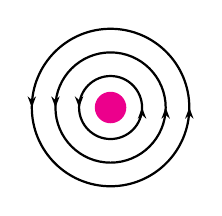
\begin{tikzpicture}[scale=0.5]
\foreach \r in {0.8,1.4,2.0} \draw[thick,postaction={decorate},decoration={markings,mark=at position 0.0 with {\arrow{Stealth[length=4pt]}},mark=at position 0.5 with {\arrow{Stealth[length=4pt]}}}] (0,0) circle (\r);
\fill[magenta] (0,0) circle (0.4);
\end{tikzpicture}\\{\small fig-Q1}
\end{minipage}\hfill
\begin{minipage}[t]{0.75\linewidth}
\begin{enumerate}
\item Field lines around a wire are shown in fig-Q1 (anticlockwise). What is the direction of the current? \mk{1M}
\answer[2]{Out of the page (towards the reader), by the right hand thumb rule.}
\end{enumerate}
\end{minipage}\\[6pt]
\begin{minipage}[t]{0.22\linewidth}\centering
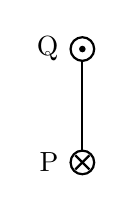
\begin{tikzpicture}[scale=0.6]
\draw[thick] (0,-1) -- (0,1);
\outpage[0.25]{(0,1.2)} \node[left] at (-0.3,1.2) {Q};
\inpage[0.25]{(0,-1.2)} \node[left] at (-0.3,-1.2) {P};
\end{tikzpicture}\\{\small fig-Q3}
\end{minipage}\hfill
\begin{minipage}[t]{0.75\linewidth}
\begin{enumerate}[start=2]
\item A coil is kept perpendicular to the page. At P the current flows into the page, at Q it comes out (fig-Q3). What is the direction of the field due to the coil? \mk{2M}
\answer[3]{At the centre, the wire at P (into page, clockwise field) gives a field to the right; the wire at Q (out of page, anticlockwise field) also gives a field to the right. So the field is along the axis of the coil, from left to right, perpendicular to the plane of the coil.}
\end{enumerate}
\end{minipage}\\[6pt]
\begin{minipage}[t]{0.22\linewidth}\centering
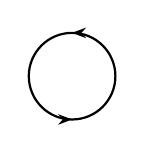
\begin{tikzpicture}[scale=0.55]
\draw[thick,postaction={decorate},decoration={markings,mark=at position 0.25 with {\arrow{Stealth[length=5pt]}},mark=at position 0.75 with {\arrow{Stealth[length=5pt]}}}] (0,0) circle (1);
\end{tikzpicture}\\{\small fig-Q4}
\end{minipage}\hfill
\begin{minipage}[t]{0.75\linewidth}
\begin{enumerate}[start=3]
\item The current in a coil flows as in fig-Q4 (anticlockwise as you see it). What pole is formed at this face? \mk{1M}
\answer[2]{North pole: curling the right-hand fingers anticlockwise, the thumb (field) points towards the viewer.}
\end{enumerate}
\end{minipage}

\exhead{C}{Label the solenoid}{\asbadge{AS5}\ \badge{2M}}
In the figure the current enters at the right end and leaves at the left. Mark the N and S ends and the direction of the field inside.
\begin{center}
\figlab{solenoid_field.png}{width=0.55\linewidth}{
\node[font=\sffamily\bfseries] at (-0.06,0.5) {\ifanswers\textcolor{anscol}{N}\else\fbox{\phantom{N}}\fi};
\node[font=\sffamily\bfseries] at (1.06,0.5) {\ifanswers\textcolor{anscol}{S}\else\fbox{\phantom{S}}\fi};
\ifanswers\draw[-{Stealth[length=6pt]},anscol,very thick] (0.75,0.5) -- (0.25,0.5) node[midway,below=6pt,font=\small]{inside: S $\to$ N};\fi}
\end{center}

\exhead{D}{Experiment}{\tb\ \asbadge{AS3}\ \badge{4M}}
Explain with the help of two activities that a current-carrying wire produces a magnetic field. \mk{4M}
\answer[12]{\textbf{Activity 1 (Oersted):} a wire stretched through the slits of two sticks is connected to a battery through a key; a compass is placed below it. When the key is closed the needle deflects; when it is opened the needle returns to N--S.\\
\textbf{Activity 4:} a vertical wire passes through a hole in a plank; 6--10 compass needles are placed on a circle around it. When the current flows, the needles set along tangents to the circle; iron filings sprinkled around form concentric circles.\\
\textbf{Conclusion:} the wire produces a magnetic field whose lines are concentric circles around it; the direction is given by the right hand thumb rule.}

\selfcheck{20}{
\item draw the field of a straight wire for both current directions
\item find the pole of a coil face from the current direction
\item describe the field of a solenoid and why its lines are closed loops}

% =====================================================================
\unit{Force on a moving charge}{\badge{1M}\ \badge{2M}\ \badge{4M}}
% =====================================================================
\begin{recall}
\begin{itemize}[leftmargin=5mm,itemsep=0pt]
\item A magnet distorts the picture on a CRT TV: the field exerts a force on the moving electrons.
\item \imp{$F=qvB\sin\theta$}; $F=qvB$ when $v\perp B$; $F=0$ when $v\parallel B$ or $v=0$.
\item Direction: right hand rule (forefinger $v$, middle finger $B$, thumb $F$), for a \textbf{positive} charge; reverse it for an electron. $F$ is always perpendicular to both $v$ and $B$.
\item A charge moving $\perp B$ goes round a circle: $r=\dfrac{mv}{Bq}$, $T=\dfrac{2\pi m}{Bq}$.
\end{itemize}
\end{recall}

\exhead{A}{Fill in the blanks}{\asbadge{AS1}\ \badge{1M}}
\begin{enumerate}
\item The force on a charge moving parallel to the field is \blank[1.5cm]{zero}.
\item The magnetic force is always perpendicular to both the \blank{velocity} and the \blank{field}.
\item For an electron, the direction of force is \blank{opposite} to that found for a positive charge.
\item The magnetic force on a charge moving $\perp B$ acts as the \blank{centripetal} force.
\end{enumerate}

\exhead{B}{Complete the derivation}{\asbadge{AS1}\ \badge{4M}}
A charge $q$ of mass $m$ moves with speed $v$ perpendicular to a uniform field $B$.\\[4pt]
(1) Magnetic force: $F=\mblank{qvB}$ \quad(since $\sin90^\circ=\mblank[1cm]{1}$).\\[4pt]
(2) This force is always perpendicular to the velocity, so the path is a \blank{circle}.\\[4pt]
(3) Centripetal force = magnetic force: \quad $\mblank{\dfrac{mv^2}{r}}=qvB$ \quad$\Rightarrow$\quad $r=\mblank[2cm]{\dfrac{mv}{Bq}}$\\[4pt]
(4) Time period $T=\dfrac{2\pi r}{v}=\mblank[2.2cm]{\dfrac{2\pi m}{Bq}}$, which does \blank{not} depend on the speed.

\exhead{C}{Numericals}{\asbadge{AS7}\ \badge{2M}}
\begin{enumerate}
\item A charge of $2\times10^{-6}$ C moves at $3\times10^4$ m/s perpendicular to $B=0.5$ T. Find the force. \mk{2M}
\answer[2]{$F=qvB=2\times10^{-6}\times3\times10^4\times0.5=3\times10^{-2}$ N.}
\item The same charge moves at $30^\circ$ to the field. Find the force. \mk{2M}
\answer[2]{$F=qvB\sin30^\circ=0.03\times\frac12=1.5\times10^{-2}$ N.}
\item A proton ($m=1.67\times10^{-27}$ kg, $q=1.6\times10^{-19}$ C) moves at $10^6$ m/s perpendicular to $B=1$ T. Find the radius of its path. \mk{2M}
\answer[3]{$r=\dfrac{mv}{Bq}=\dfrac{1.67\times10^{-27}\times10^6}{1\times1.6\times10^{-19}}=1.04\times10^{-2}$ m $\approx1$ cm.}
\end{enumerate}

\exhead{D}{Short answers}{\tb\ \asbadge{AS1}\ \badge{2M}}
\begin{enumerate}
\item Why does the picture appear distorted when a bar magnet is brought close to the screen of a television? \mk{2M}
\answer[3]{The picture on a CRT screen is made by a beam of fast-moving electrons. The magnet's field exerts a force $F=qvB\sin\theta$ on them, which changes their path, so they strike the wrong spots and the picture is distorted.}
\item State the right hand rule for the direction of force on a positive charge. \mk{2M}
\answer[3]{Stretch the thumb, forefinger and middle finger of the right hand mutually perpendicular. If the forefinger points along the velocity (or current) and the middle finger along the field, the thumb gives the direction of the force.}
\end{enumerate}

\selfcheck{25}{
\item use $F=qvB\sin\theta$ including the zero-force cases
\item find the direction of force with the right hand rule, and reverse it for electrons
\item derive $r=mv/Bq$ and $T=2\pi m/Bq$}

% =====================================================================
\unit{Force on a current; electric motor}{\badge{1M}\ \badge{2M}\ \badge{4M}}
% =====================================================================
\begin{recall}
\begin{itemize}[leftmargin=5mm,itemsep=0pt]
\item A current is moving charge, so a current-carrying wire in a field feels a force: \imp{$F=ILB\sin\theta$}; $F=ILB$ when $I\perp B$; $F=0$ when $I\parallel B$.
\item Activity 8: a wire in a horseshoe magnet is deflected; reversing the current or the poles reverses the deflection.
\item \key{Motor}: forces on opposite sides of a coil are equal and opposite (net force 0) but form a \textbf{couple} that rotates the coil. \textbf{Split rings} and brushes reverse the current every half turn. Electrical $\to$ mechanical energy.
\end{itemize}
\end{recall}

\exhead{A}{Complete the derivation of $F=ILB$}{\asbadge{AS1}\ \badge{4M}}
(1) Force on one charge moving with drift velocity $v$ perpendicular to $B$: $F_0=\mblank{qvB}$.\\[4pt]
(2) Total charge in the length $L$ inside the field is $Q$: $F=\mblank{QvB}$ \dots(1)\\[4pt]
(3) Time to cross length $L$: $t=\dfrac{L}{v}$, so $v=\mblank{\dfrac{L}{t}}$ \dots(2)\\[4pt]
(4) Put (2) in (1): $F=\mblank[2.2cm]{\dfrac{Q}{t}LB}$ \dots(3)\\[4pt]
(5) Since $\dfrac{Q}{t}=\mblank[1cm]{I}$, \quad $F=\mblank[1.6cm]{ILB}$. At an angle $\theta$: $F=\mblank[2cm]{ILB\sin\theta}$.

\exhead{B}{Numericals}{\tb\ \asbadge{AS7}\ \badge{2M}}
\begin{enumerate}
\item \tb\ An 8 N force acts on a 20 cm conductor placed perpendicular to a magnetic field. The current is 40 A. Find the magnetic field induction. \mk{2M}
\answer[3]{$L=0.2$ m. $B=\dfrac{F}{IL}=\dfrac{8}{40\times0.2}=1$ T.}
\item A wire 0.5 m long carries 4 A at $30^\circ$ to a field of 0.2 T. Find the force. \mk{2M}
\answer[2]{$F=ILB\sin30^\circ=4\times0.5\times0.2\times\frac12=0.2$ N.}
\end{enumerate}

\exhead{C}{Direction of force}{\tb\ \asbadge{AS1}\ \badge{2M}}
\noindent
\begin{minipage}[c]{0.3\linewidth}\centering
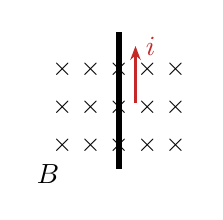
\begin{tikzpicture}[scale=0.6]
\foreach \x in {-2,...,2}{\foreach \y in {-1,...,1}{\node[font=\small] at (\x*0.6,\y*0.8) {$\times$};}}
\draw[line width=2pt] (0,-1.3) -- (0,1.6);
\draw[cur] (0.35,0.1) -- (0.35,1.3) node[right]{$i$};
\node at (-1.5,-1.4) {$B$};
\end{tikzpicture}\\{\small fig-Q5}
\end{minipage}\hfill
\begin{minipage}[c]{0.67\linewidth}
A straight wire carrying current $i$ upward is kept perpendicular to a field directed into the page; length $L$ is in the field. Find the magnitude and direction of the force. \mk{2M}
\answer[3]{Magnitude $F=iLB$ (since $\theta=90^\circ$). Right hand rule: forefinger up ($i$), middle finger into the page ($B$) $\Rightarrow$ thumb points to the \textbf{left}. The force acts to the left, in the plane of the page.}
\end{minipage}

\exhead{D}{Motor}{\asbadge{AS1}\ \asbadge{AS5}\ \badge{4M}}
\noindent
\begin{minipage}[c]{0.38\linewidth}\centering
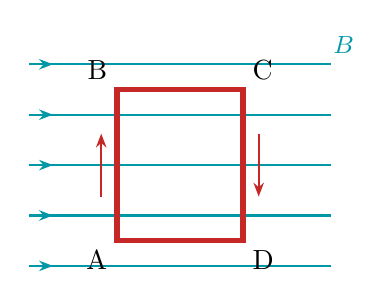
\begin{tikzpicture}[scale=0.8]
\foreach \y in {-1.6,-0.8,0,0.8,1.6} \draw[fl=0.08] (-2.4,\y) -- (2.4,\y);
\node[font=\small\bfseries,fieldc] at (2.6,1.9) {$B$};
\draw[ecred,line width=2pt] (-1,-1.2) -- (-1,1.2) -- (1,1.2) -- (1,-1.2) -- cycle;
\draw[cur] (-1.25,-0.5) -- (-1.25,0.5); \draw[cur] (1.25,0.5) -- (1.25,-0.5);
\node[below left] at (-1,-1.2) {A}; \node[above left] at (-1,1.2) {B};
\node[above right] at (1,1.2) {C}; \node[below right] at (1,-1.2) {D};
\end{tikzpicture}
\end{minipage}\hfill
\begin{minipage}[c]{0.6\linewidth}
\begin{enumerate}
\item The force on AB is directed \blank{into the page} and on CD \blank{out of the page}.\mk{1M}
\item The net force on the coil is \blank[1.5cm]{zero}, yet the coil \blank{rotates} because the two forces form a \blank{couple}. \mk{1M}
\item Why is the current reversed every half turn, and which part does it? \mk{2M}
\answer[3]{After half a turn the forces would turn the coil back, so it would only rock to and fro. The split rings (commutator), rotating with the coil, swap brushes every half turn, reversing the current so the rotation continues in the same direction.}
\end{enumerate}
\end{minipage}

\exhead{E}{Experiment}{\tb\ \asbadge{AS3}\ \badge{4M}}
How do you verify experimentally that a current-carrying conductor experiences a force when kept in a magnetic field? \mk{4M}
\answer[10]{\textbf{Materials:} wooden plank, two split sticks, copper wire, 9 V battery, switch, horseshoe magnet.\\
\textbf{Procedure:} pass the wire through the splits of the sticks and connect it to the battery through the switch. Close the switch and bring the horseshoe magnet so the wire lies between its poles.\\
\textbf{Observation:} the wire is deflected (pushed up or down). Reversing the poles of the magnet, or the direction of the current, reverses the deflection.\\
\textbf{Conclusion:} a current-carrying conductor in a field experiences a force $F=ILB$; its direction is given by the right hand rule.}

\selfcheck{27}{
\item derive $F=ILB$ from $F=qvB$
\item find the direction of force on a wire with the right hand rule
\item explain the working of a motor, including split rings}

% =====================================================================
\unit{Induction: Faraday, Lenz and motional emf}{\badge{1M}\ \badge{2M}\ \badge{4M}}
% =====================================================================
\begin{recall}
\begin{itemize}[leftmargin=5mm,itemsep=0pt]
\item \key{Electromagnetic induction}: a current is induced in a coil when the flux through it changes (relative motion of magnet and coil).
\item \key{Faraday's law}: $\varepsilon=\dfrac{\Delta\Phi}{\Delta t}$; for $N$ turns $\varepsilon=N\dfrac{\Delta\Phi_0}{\Delta t}$.
\item \key{Lenz's law}: the induced current opposes the change in flux (conservation of energy). N pole approaching $\Rightarrow$ near face of coil becomes N.
\item \key{Motional emf}: $\varepsilon=Blv$ for a conductor of length $l$ moving with speed $v$ perpendicular to $B$.
\end{itemize}
\end{recall}

\exhead{A}{Activity 9: what does the galvanometer show?}{\asbadge{AS3}\ \badge{1M}}
\renewcommand{\arraystretch}{1.7}
\begin{tabularx}{\linewidth}{>{\small}X>{\small}X}
\toprule
\rowcolor{ecblue}\textcolor{white}{\textbf{Action}} & \textcolor{white}{\textbf{Galvanometer}}\\
\midrule
Magnet held at rest inside the coil & \blank{no deflection}\\
N pole pushed towards the coil & \blank{deflects one way}\\
N pole pulled away from the coil & \blank{deflects the opposite way}\\
S pole pushed towards the coil & \blank{deflects opposite to N pushed in}\\
Magnet pushed in faster & \blank{larger deflection}\\
\bottomrule
\end{tabularx}

\exhead{B}{Fill in the blanks}{\asbadge{AS1}\ \badge{1M}}
\begin{enumerate}
\item The current produced by changing flux is called the \blank{induced current}.
\item Lenz's law is a consequence of the conservation of \blank{energy}.
\item When the N pole of a magnet approaches a coil, the face of the coil nearer to it becomes a \blank[1.5cm]{north} pole.
\item $\varepsilon=Blv$ is called the \blank{motional emf}.
\end{enumerate}

\exhead{C}{Complete the derivation of $\varepsilon=Blv$}{\asbadge{AS1}\ \badge{4M}}
A cross wire of length $l$ lies on two parallel conductors in a uniform field $B$. It is moved a distance $s$ in time $\Delta t$ and a current $I$ flows.\\[4pt]
(1) Force of the field on the cross wire: $F=\mblank{BIl}$ \dots(8)\\[4pt]
(2) Work done by us in moving it: $W=Fs=\mblank{BIls}$ \dots(9)\\[4pt]
(3) Change in flux as the loop area changes by $ls$: $\Delta\Phi=\mblank{Bls}$ \dots(10) \;$\Rightarrow W=\mblank{I\,\Delta\Phi}$\\[4pt]
(4) Dividing by $\Delta t$: $P=\dfrac{W}{\Delta t}=\mblank{\dfrac{I\Delta\Phi}{\Delta t}}$; comparing with $P=\varepsilon I$ gives $\varepsilon=\mblank{\dfrac{\Delta\Phi}{\Delta t}}$\\[4pt]
(5) Also $P=Fv=\mblank{BIlv}$ (since $\dfrac{s}{\Delta t}=v$). So $\varepsilon I=BIlv$ \;$\Rightarrow\;\varepsilon=\mblank[1.6cm]{Blv}$

\exhead{D}{Numericals}{\tb\ \asbadge{AS7}\ \badge{2M}}
\begin{worked}[Worked example (textbook): 400 turns, flux per turn rises by 0.001 Wb in 0.1 s]
$\varepsilon=N\dfrac{\Delta\Phi_0}{\Delta t}=\dfrac{400\times0.001}{0.1}=4$ V. While the flux stays constant (0.1 s to 0.3 s), $\varepsilon=0$.
\end{worked}
\begin{enumerate}
\item \tb\ Find the length of a conductor moving at 10 m/s perpendicular to a field of 0.8 T if it induces an emf of 8 V. \mk{2M}
\answer[2]{$l=\dfrac{\varepsilon}{Bv}=\dfrac{8}{0.8\times10}=1$ m.}
\item The flux per turn in a coil of 100 turns falls from 0.05 Wb to 0.01 Wb in 0.2 s. Find the induced emf. \mk{2M}
\answer[3]{$\Delta\Phi_0=0.04$ Wb. $\varepsilon=\dfrac{100\times0.04}{0.2}=20$ V.}
\item A 1.5 m rod moves at 2 m/s perpendicular to $B=0.4$ T. Find the emf. \mk{2M}
\answer[2]{$\varepsilon=Blv=0.4\times1.5\times2=1.2$ V.}
\end{enumerate}

\exhead{E}{Figure questions}{\tb\ \asbadge{AS1}\ \asbadge{AS2}\ \badge{2M}}
\noindent
\begin{minipage}[c]{0.3\linewidth}\centering
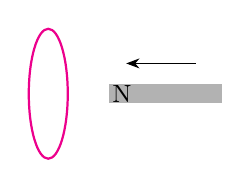
\begin{tikzpicture}[scale=0.55]
\draw[magenta,thick] (0,0) ellipse (0.45 and 1.5);
\fill[gray!60] (1.4,-0.22) rectangle (4,0.22); \node[font=\small] at (1.7,0) {N};
\draw[-{Stealth}] (3.4,0.7) -- (1.8,0.7);
\end{tikzpicture}\\{\small fig-Q2}
\end{minipage}\hfill
\begin{minipage}[c]{0.67\linewidth}
\begin{enumerate}
\item A bar magnet with its N pole facing a coil moves towards it (fig-Q2). What happens to the flux through the coil? Which way does the induced current flow as seen from the magnet? \mk{2M}
\answer[3]{The flux through the coil increases. By Lenz's law the near face becomes N to repel the magnet, so the induced current is anticlockwise as seen from the magnet.}
\end{enumerate}
\end{minipage}\\[6pt]
\begin{minipage}[c]{0.3\linewidth}\centering
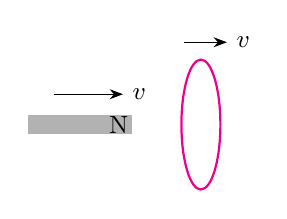
\begin{tikzpicture}[scale=0.55]
\fill[gray!60] (-3,-0.22) rectangle (-0.6,0.22); \node[font=\small] at (-0.9,0) {N};
\draw[-{Stealth}] (-2.4,0.7) -- (-0.8,0.7) node[right,font=\small]{$v$};
\draw[magenta,thick] (1,0) ellipse (0.45 and 1.5);
\draw[-{Stealth}] (0.6,1.9) -- (1.6,1.9) node[right,font=\small]{$v$};
\end{tikzpicture}\\{\small fig-Q6}
\end{minipage}\hfill
\begin{minipage}[c]{0.67\linewidth}
\begin{enumerate}[start=2]
\item \tb\ The coil and the bar magnet both move in the same direction with the same speed (fig-Q6). What happens? \mk{2M}
\answer[3]{There is no relative motion between the magnet and the coil, so the flux through the coil does not change. No emf is induced and no current flows.}
\end{enumerate}
\end{minipage}

\exhead{F}{Long answers}{\tb\ \asbadge{AS1}\ \asbadge{AS3}\ \badge{4M}}
\begin{enumerate}
\item Explain Faraday's law of induction with the help of an activity. \mk{4M}
\answer[10]{\textbf{Activity:} connect a coil to a galvanometer. Push the N pole of a bar magnet into the coil: the needle deflects. Hold it still: no deflection. Pull it out: the needle deflects the other way. With the S pole the deflections reverse. Moving the coil instead of the magnet gives the same result; faster motion gives a larger deflection.\\
\textbf{Law:} whenever the magnetic flux linked with a closed coil changes, an emf (and current) is induced. The induced emf equals the rate of change of flux: $\varepsilon=\dfrac{\Delta\Phi}{\Delta t}$; for $N$ turns, $\varepsilon=N\dfrac{\Delta\Phi_0}{\Delta t}$.}
\item State Lenz's law and show that it follows from the conservation of energy. \mk{4M}
\answer[9]{\textbf{Law:} the induced current flows in a direction that opposes the change in flux producing it.\\
\textbf{Energy argument:} push the N pole towards a coil. If the induced current made the near face S, it would attract the magnet, which would speed up by itself while electrical energy was also produced: energy from nothing, which is impossible. So the near face must be N and repel the magnet; we must do work to push it, and this work becomes electrical energy. Pulling the magnet away, the near face becomes S and attracts it, again opposing the motion.}
\item What experiment do you suggest to understand Faraday's law? What instruments are required? Give suggestions for good results and precautions. \mk{4M}
\answer[9]{\textbf{Experiment:} Activity 9 (magnet moved in and out of a coil connected to a galvanometer).\\
\textbf{Instruments:} coil of many turns of insulated copper wire, strong bar magnet, sensitive galvanometer, connecting wires.\\
\textbf{For good results:} use more turns, a stronger magnet and faster motion.\\
\textbf{Precautions:} tight connections; keep the galvanometer away from the magnet; check the zero before starting; move the magnet along the axis of the coil; do not drop the magnet.}
\end{enumerate}

\selfcheck{44}{
\item describe Activity 9 and state Faraday's law
\item state Lenz's law and give the energy argument
\item derive $\varepsilon=\Delta\Phi/\Delta t$ and $\varepsilon=Blv$
\item solve induced-emf numericals with $N$ turns}

% =====================================================================
\unit{Applications, levitation and generators}{\badge{1M}\ \badge{2M}\ \badge{4M}}
% =====================================================================
\begin{recall}
\begin{itemize}[leftmargin=5mm,itemsep=0pt]
\item Applications of induction: security metal detectors, tape recorder heads, induction stoves, ATM card readers.
\item \key{Levitation}: AC in a coil around an iron core $\Rightarrow$ changing flux through a metal ring $\Rightarrow$ induced current opposes it $\Rightarrow$ repulsion balances the ring's weight. With DC the ring only jumps at switch on/off.
\item \key{AC generator}: coil rotated in a field; full \textbf{slip rings}; emf zero when the coil is vertical, maximum when horizontal; reverses every half turn. \key{DC generator}: half (split) rings keep the output in one direction. Mechanical $\to$ electrical energy.
\end{itemize}
\end{recall}

\exhead{A}{Match the following}{\asbadge{AS1}\ \badge{1M}}
\renewcommand{\arraystretch}{1.3}
\begin{tabularx}{\linewidth}{@{}l l c X@{}}
\toprule
& \textbf{Column A} & & \textbf{Column B}\\
\midrule
1. & Induction stove & \bx{c} & a) Induced current in a large coil triggers an alarm\\
2. & Security check & \bx{a} & b) Magnetised tape moves past a small coil\\
3. & Tape recorder & \bx{b} & c) Induced current heats a metal pan\\
4. & Electric motor & \bx{e} & d) Mechanical energy into electrical energy\\
5. & Generator & \bx{d} & e) Electrical energy into mechanical energy\\
\bottomrule
\end{tabularx}

\exhead{B}{Levitation}{\asbadge{AS1}\ \asbadge{AS7}\ \badge{2M}\ \badge{4M}}
\begin{enumerate}
\item Why does the metal ring levitate when AC is used? \mk{4M}
\answer[8]{The ring is at rest, so the net force on it is zero: an upward force balances its weight. AC changes in size and direction continuously, so the flux through the ring keeps changing and a current is induced in it (Faraday). By Lenz's law this current opposes the change, so the ring's lower face always has the same polarity as the coil's upper face (e.g.\ coil top S, ring bottom S). The repulsion provides the upward force that holds the ring up.}
\item What happens if DC is used instead of AC? Why? \mk{2M}
\answer[3]{The ring jumps up only when the switch is closed (and again when it is opened) and then falls back, because the flux through the ring changes only at those instants. With a steady current there is no change of flux, no induced current and no repulsion.}
\end{enumerate}

\exhead{C}{AC generator}{\asbadge{AS1}\ \asbadge{AS5}\ \badge{2M}\ \badge{4M}}
\begin{enumerate}
\item Sketch the emf produced by an AC generator over one rotation, starting with the coil vertical. Mark where the emf is zero and maximum. \mk{2M}
\drawbox{4.5cm}{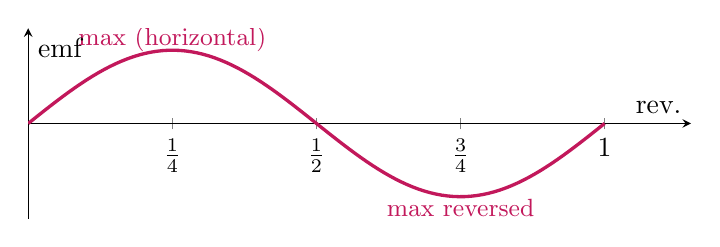
\begin{tikzpicture}
\begin{axis}[width=10cm,height=4cm,axis lines=middle,xmin=0,xmax=1.15,ymin=-1.3,ymax=1.3,
  xtick={0.25,0.5,0.75,1},xticklabels={$\frac14$,$\frac12$,$\frac34$,1},ytick=\empty,xlabel={rev.},ylabel={emf}]
\addplot[anscol,very thick,domain=0:1,samples=100] {sin(deg(2*pi*x))};
\node[font=\small,anscol] at (axis cs:0.25,1.15) {max (horizontal)};
\node[font=\small,anscol] at (axis cs:0.75,-1.15) {max reversed};
\end{axis}\end{tikzpicture}\\\small Zero at 0, $\frac12$, 1 rotation (coil vertical); maximum at $\frac14$ and $\frac34$ (coil horizontal).}
\item Why does the emf vary from zero to maximum during a rotation? \mk{2M}
\answer[3]{The emf depends on how fast the flux through the coil changes. When the coil is vertical (plane $\perp$ field) the flux is maximum but changing slowest, so the emf is zero. When it is horizontal (plane $\parallel$ field) the flux is changing fastest, so the emf is maximum.}
\item How is an AC generator converted into a DC generator? \mk{2M}
\answer[3]{Replace the two full slip rings by two half (split) rings. After every half rotation the ends of the coil change brushes, so the current in the external circuit always flows in the same direction (DC).}
\end{enumerate}

\exhead{D}{Textbook application}{\tb\ \asbadge{AS7}\ \badge{2M}}
Give a few applications of Faraday's law of induction in daily life. \mk{2M}
\answer[4]{Electric generators in power stations; metal detectors at security checks; tape recorder heads; induction stoves; ATM/credit card readers; transformers; bicycle dynamo.}

\selfcheck{25}{
\item explain four applications of induction
\item explain levitation with AC and why DC fails
\item explain the AC generator, its emf graph and the DC version}

% =====================================================================
\clearpage
\section*{\sffamily\color{ecblue}One-mark rapid fire}
{\small Answer in one word or one line. Target \textbf{8 minutes} for 25 questions.}\hfill Time taken: \rule{1.6cm}{0.3pt}\qquad Score: \rule{1cm}{0.3pt} / 25
\vspace{4pt}
\renewcommand{\arraystretch}{1.55}
\begin{multicols}{2}
\begin{enumerate}[itemsep=5pt]
\item Discovered the magnetic effect of current? \blank[2cm]{Oersted}
\item Unit of magnetic flux? \blank[2cm]{weber}
\item Unit of flux density? \blank[2cm]{tesla}
\item 1 T in N, A, m? \blank[2cm]{N/(A m)}
\item $\Phi$ for a plane $\parallel B$? \blank[2cm]{zero}
\item Field lines of a straight wire? \blank[2cm]{circles}
\item Current $\odot$: field lines are? \blank[2cm]{anticlockwise}
\item Rule for field of a wire? \blank[2cm]{thumb rule}
\item Anticlockwise current face is? \blank[2cm]{N pole}
\item Coil that acts like a bar magnet? \blank[2cm]{solenoid}
\item Force on a charge moving $\parallel B$? \blank[2cm]{zero}
\item Formula for force on a charge? \blank[2cm]{$qvB\sin\theta$}
\item Radius of path of a charge? \blank[2cm]{$mv/Bq$}
\item Force on a current $\perp B$? \blank[2cm]{$ILB$}
\item Motor converts? \blank[2cm]{elec.\ $\to$ mech.}
\item Reverses current in a motor? \blank[2cm]{split rings}
\item Faraday's law formula? \blank[2cm]{$\Delta\Phi/\Delta t$}
\item Law giving induced current direction? \blank[2cm]{Lenz's law}
\item Lenz's law is based on? \blank[2cm]{energy cons.}
\item Motional emf? \blank[2cm]{$Blv$}
\item Emf when coil plane $\perp B$ (generator)? \blank[2cm]{zero}
\item Rings in an AC generator? \blank[2cm]{slip rings}
\item Generator converts? \blank[2cm]{mech.\ $\to$ elec.}
\item Stove using induction? \blank[2cm]{induction stove}
\item Current reversing periodically? \blank[2cm]{AC}
\end{enumerate}
\end{multicols}

% =====================================================================
\clearpage
\section*{\sffamily\color{ecblue}Score boosters}
\subsection*{\sffamily Anatomy of a full-marks 4-mark answer}
{\small Example question: \emph{Explain the working of an electric motor.}}\par\vspace{2pt}
\renewcommand{\arraystretch}{1.5}
\begin{tabularx}{\linewidth}{>{\bfseries\sffamily\small}p{2.6cm}X>{\small}p{2.7cm}}
\toprule
\rowcolor{ecteal!15}Part & \textbf{What to write} & \textbf{Why it matters}\\
\midrule
1. Principle & A current-carrying coil in a field experiences a force ($F=ILB$). & Scores the concept mark.\\
2. Diagram & Coil ABCD between N and S, split rings, brushes, battery; arrows for current. & Diagrams carry marks.\\
3. Forces & AB and CD: equal, opposite forces $\Rightarrow$ couple $\Rightarrow$ rotation. & Shows you know why.\\
4. Commutator & Split rings reverse current every half turn $\Rightarrow$ continuous rotation. & Key idea examiners look for.\\
5. Energy & Electrical energy $\to$ mechanical energy. & Closes the answer.\\
\bottomrule
\end{tabularx}

\subsection*{\sffamily Keywords the examiner looks for}
\renewcommand{\arraystretch}{1.35}
\begin{tabularx}{\linewidth}{>{\bfseries\small}p{3.8cm}>{\small}X}
\toprule
Oersted & compass deflects $\cdot$ current produces field\\
Field lines & tangent gives direction $\cdot$ crowded = strong $\cdot$ closed loops\\
Straight wire & concentric circles $\cdot$ right hand thumb rule\\
Force & $qvB\sin\theta$ $\cdot$ $ILB\sin\theta$ $\cdot$ zero when parallel $\cdot$ right hand rule\\
Motor & couple $\cdot$ split rings $\cdot$ brushes $\cdot$ electrical to mechanical\\
Faraday & change of flux $\cdot$ rate of change $\cdot$ induced emf\\
Lenz & opposes the change $\cdot$ conservation of energy\\
Generator & rotating coil $\cdot$ slip rings $\cdot$ zero/maximum emf $\cdot$ mechanical to electrical\\
\bottomrule
\end{tabularx}

\begin{examtip}[Mistakes that cost marks]
\begin{multicols}{2}\small
\begin{itemize}[leftmargin=4mm,itemsep=1pt]
\item Field lines without arrows.
\item $\theta$ measured from the plane, not the normal, in $\Phi=BA\cos\theta$.
\item Forgetting $F=0$ when parallel to $B$.
\item Not reversing the force for an electron.
\item Using cm or cm$^2$ without converting.
\item Forgetting $N$ in $\varepsilon=N\Delta\Phi_0/\Delta t$.
\item Slip rings in a motor (it has split rings).
\item No energy argument in Lenz's law.
\end{itemize}
\end{multicols}
\end{examtip}

\subsection*{\sffamily Formula sheet \normalfont\small(cover the right column and test yourself)}
\renewcommand{\arraystretch}{1.7}
\begin{tabularx}{\linewidth}{>{\bfseries\small}p{5.3cm}X}
\toprule
\rowcolor{ecred}\textcolor{white}{Quantity} & \textcolor{white}{\textbf{Formula / unit}}\\
\midrule
Flux density & $B=\dfrac{\Phi}{A}$ \quad tesla = Wb/m$^2$\\
Flux & $\Phi=BA\cos\theta$ \quad weber\\
Force on a charge & $F=qvB\sin\theta$\\
Circular motion & $r=\dfrac{mv}{Bq}$,\quad $T=\dfrac{2\pi m}{Bq}$\\
Force on a current & $F=ILB\sin\theta$\\
Faraday's law & $\varepsilon=\dfrac{\Delta\Phi}{\Delta t}$;\quad $\varepsilon=N\dfrac{\Delta\Phi_0}{\Delta t}$\\
Motional emf & $\varepsilon=Blv$\\
\bottomrule
\end{tabularx}

\subsection*{\sffamily Diagram practice tracker}
{\small Draw each diagram three times on separate days. Tick when you can draw it from memory in under 4 minutes.}\par
\renewcommand{\arraystretch}{1.4}
\begin{tabularx}{\linewidth}{X c c c}
\toprule
\textbf{Diagram} & \textbf{Try 1} & \textbf{Try 2} & \textbf{Try 3}\\
\midrule
Field lines of a bar magnet & \tick & \tick & \tick\\
Field of a straight wire ($\odot$ and $\otimes$) & \tick & \tick & \tick\\
Field of a solenoid with N and S & \tick & \tick & \tick\\
Right hand rule for force & \tick & \tick & \tick\\
Electric motor with split rings & \tick & \tick & \tick\\
Faraday's activity (magnet, coil, galvanometer) & \tick & \tick & \tick\\
AC generator and emf graph & \tick & \tick & \tick\\
\bottomrule
\end{tabularx}

% =====================================================================
\clearpage
\section*{\sffamily\color{ecblue}Chapter test}
\begin{tcolorbox}[wbox,colback=ecblue!5,colframe=ecblue]
\sffamily\small\textbf{Time: 1 hour 30 minutes \hfill Maximum marks: 40}\\[2pt]
\rmfamily Section I: 6 questions $\times$ 1 mark. Section II: 5 questions $\times$ 2 marks. Section III: 4 questions $\times$ 4 marks, each with an internal choice. Section IV: 8 multiple choice questions $\times$ 1 mark.
\end{tcolorbox}

\exhead{Section I}{}{\badge{6 $\times$ 1 = 6}}
\begin{enumerate}
\item What is the SI unit of magnetic flux density? \answer[1]{Tesla (Wb/m$^2$).}
\item State Lenz's law. \answer[1]{The induced current opposes the change in flux producing it.}
\item What is the force on a current-carrying wire kept parallel to a magnetic field? \answer[1]{Zero.}
\item Which device converts mechanical energy into electrical energy? \answer[1]{Generator.}
\item Write the formula for motional emf. \answer[1]{$\varepsilon=Blv$.}
\item Name the rule used to find the direction of the field around a straight wire. \answer[1]{Right hand thumb rule.}
\end{enumerate}

\exhead{Section II}{}{\badge{5 $\times$ 2 = 10}}
\begin{enumerate}[resume]
\item Why does a TV picture get distorted when a magnet is brought near it? \answer[3]{The picture is made by moving electrons; the magnet's field exerts a force on them and deflects them.}
\item A 0.5 m wire carries 2 A perpendicular to a field of 0.4 T. Find the force. \answer[2]{$F=ILB=2\times0.5\times0.4=0.4$ N.}
\item A coil of 50 turns has its flux per turn changed by 0.02 Wb in 0.1 s. Find the induced emf. \answer[2]{$\varepsilon=\frac{50\times0.02}{0.1}=10$ V.}
\item Are magnetic field lines closed? Explain. \answer[3]{Yes: circles round a wire; for a solenoid/magnet the lines go N $\to$ S outside and S $\to$ N inside.}
\item A coil and a magnet move together in the same direction at the same speed. Is a current induced? Why? \answer[3]{No: no relative motion, so no change of flux.}
\end{enumerate}

\exhead{Section III}{}{\badge{4 $\times$ 4 = 16}}
\begin{enumerate}[resume]
\item Explain with two activities that a current-carrying wire produces a magnetic field.\\
\textbf{OR}\quad Describe an activity to show that a current-carrying wire experiences a force in a magnetic field.
\answer[8]{See Unit 3, Exercise D or Unit 5, Exercise E.}
\item Derive $F=ILB$ for a straight wire in a magnetic field.\\
\textbf{OR}\quad Derive $r=\dfrac{mv}{Bq}$ and $T=\dfrac{2\pi m}{Bq}$ for a charge moving perpendicular to a field.
\answer[8]{See Unit 5, Exercise A or Unit 4, Exercise B.}
\item Derive $\varepsilon=Blv$ using conservation of energy.\\
\textbf{OR}\quad State Faraday's law and explain it with an activity.
\answer[8]{See Unit 6, Exercise C or Exercise F1.}
\item Explain the working of an electric motor with a diagram.\\
\textbf{OR}\quad Explain the working of an AC generator with the graph of emf for one rotation.
\answer[8]{See the anatomy table in Score boosters (motor) or Unit 7, Exercise C.}
\end{enumerate}

\exhead{Section IV}{}{\badge{8 $\times$ 1 = 8}}
\begin{enumerate}[resume]
\mcq{Which converts electrical energy into mechanical energy?}{motor}{battery}{generator}{switch}{A}
\mcq{The force on a wire perpendicular to a uniform field is}{0}{$ILB$}{$2ILB$}{$ILB/2$}{B}
\mcq{One tesla is equal to}{N/C}{N/(A m)}{A/m}{N/(A s)}{B}
\mcq{Unit of magnetic flux is}{dyne}{oersted}{gauss}{weber}{D}
\mcq{No force acts on a current-carrying conductor kept}{parallel to the field}{perpendicular to the field}{in the field}{away from the field}{A}
\mcq{Current flows anticlockwise in a coil as you see it. The face towards you is}{S pole}{N pole}{neither}{both}{B}
\mcq{In an AC generator the emf is maximum when the plane of the coil is}{perpendicular to $B$}{parallel to $B$}{at $45^\circ$}{at rest}{B}
\mcq{The time period of a charge moving in a circle in a uniform field depends on}{its speed}{the radius}{$m$, $q$ and $B$}{none}{C}
\end{enumerate}

\vspace{6pt}
\begin{tcolorbox}[wbox,colback=ecgold!10,colframe=ecorange,title={\faChartLine\ My test result}]
\renewcommand{\arraystretch}{1.6}
\begin{tabularx}{\linewidth}{X c c c c c}
Section & I & II & III & IV & \textbf{Total}\\
Marks & \rule{0.9cm}{0.3pt}\,/6 & \rule{0.9cm}{0.3pt}\,/10 & \rule{0.9cm}{0.3pt}\,/16 & \rule{0.9cm}{0.3pt}\,/8 & \rule{0.9cm}{0.3pt}\,/40\\
\end{tabularx}
\end{tcolorbox}

% =====================================================================
\clearpage
\section*{\sffamily\color{ecblue}Mistake log}
{\small Write every question you got wrong. Redo it after one week without looking at the answer.}\par\vspace{4pt}
\renewcommand{\arraystretch}{2.5}
\begin{tabularx}{\linewidth}{|p{1.4cm}|X|X|c|}
\hline
\rowcolor{ecblue!12}\textbf{Unit / Q} & \textbf{What I wrote} & \textbf{The correct idea} & \textbf{Redone}\\\hline
\logrow\logrow\logrow\logrow\logrow\logrow\logrow\logrow\logrow\logrow\logrow\logrow\logrow\logrow
\end{tabularx}

\end{document}
"
\documentclass[11pt,a4paper]{article}
\usepackage[a4paper,margin=17mm,top=20mm,bottom=20mm,headsep=6mm]{geometry}
\usepackage[T1]{fontenc}
\usepackage{newtxtext,newtxmath}
\usepackage{amsmath}
\usepackage{graphicx}
\usepackage{tikz}
\usetikzlibrary{arrows.meta,calc,decorations.markings}
\usepackage[american]{circuitikz}
\usepackage{pgfplots}
\pgfplotsset{compat=1.18}
\usepackage[most]{tcolorbox}
\usepackage{booktabs,array,tabularx,multicol}
\usepackage[table]{xcolor}
\usepackage{enumitem}
\usepackage{fontawesome5}
\usepackage[normalem]{ulem}
\usepackage{fancyhdr}
\usepackage{xparse}
\graphicspath{{figures/}}

% ---------------- edition switch ----------------
\newif\ifanswers
\ifdefined\withanswers\answerstrue\fi

% ---------------- colours (same as the classroom deck) ----------------
\definecolor{ecblue}{HTML}{1F4E9A}
\definecolor{ecteal}{HTML}{0E8C8C}
\definecolor{ecorange}{HTML}{E8710A}
\definecolor{ecred}{HTML}{C62828}
\definecolor{ecgreen}{HTML}{2E7D32}
\definecolor{ecpurple}{HTML}{6A1B9A}
\definecolor{ecgold}{HTML}{F9A825}
\definecolor{ecnavy}{HTML}{0D2B5E}
\definecolor{anscol}{HTML}{C2185B}
\definecolor{rulecol}{HTML}{9AA7BD}

\setlength{\parindent}{0pt}
\setlength{\parskip}{3pt}
\setlist{itemsep=3pt,topsep=3pt}
\setlist[enumerate,1]{label=\textbf{\arabic*.},leftmargin=7mm}

% ---------------- header / footer ----------------
\pagestyle{fancy}
\fancyhf{}
\renewcommand{\headrulewidth}{0.4pt}
\fancyhead[L]{\small\sffamily\color{ecblue}Magnetic Effects of Electric Current \;$\cdot$\; Workbook}
\fancyhead[R]{\small\sffamily\ifanswers\textcolor{anscol}{\textbf{ANSWER KEY}}\;$\cdot$\;\fi Class X Physical Science}
\fancyfoot[C]{\small\sffamily\thepage}
\fancyfoot[R]{\ifanswers\else\scriptsize\sffamily\color{gray}Name: \rule{3.5cm}{0.3pt}\fi}

% ---------------- building blocks ----------------
\newcommand{\badge}[1]{\tikz[baseline=(b.base)]\node[fill=ecgold,text=black,rounded corners=2.5pt,
  inner sep=2pt,font=\sffamily\scriptsize\bfseries](b){#1};}
\newcommand{\asbadge}[1]{\tikz[baseline=(b.base)]\node[draw=ecteal,text=ecteal,rounded corners=2.5pt,
  inner sep=1.6pt,font=\sffamily\scriptsize\bfseries](b){#1};}
\newcommand{\tb}{\tikz[baseline=(b.base)]\node[fill=ecblue,text=white,rounded corners=2.5pt,
  inner sep=1.8pt,font=\sffamily\scriptsize\bfseries](b){Textbook};}
\newcommand{\imp}[1]{\textcolor{ecred}{\textbf{#1}}}
\newcommand{\key}[1]{\textcolor{ecblue}{\textbf{#1}}}
\newcommand{\mk}[1]{\hfill\badge{#1}}
\newcommand{\tick}{\faSquare[regular]}
\newcommand{\logrow}{ & & & \tick\\\hline}
\newcommand{\bx}[1]{[\,\makebox[1em]{\ifanswers\textcolor{anscol}{\textbf{#1}}\fi}\,]}

% blank for a word or phrase
\newcommand{\blank}[2][2.8cm]{\ifanswers\leavevmode{\color{anscol}\bfseries\uline{#2}}\else\rule[-2pt]{#1}{0.5pt}\fi}
% blank inside mathematics
\newcommand{\mblank}[2][1.8cm]{\ifanswers\leavevmode{\color{anscol}\ensuremath{#2}}\else\ensuremath{\underline{\hspace{#1}}}\fi}
% ruled writing lines
\newcommand{\writelines}[1]{\par\foreach\n in {1,...,#1}{\vspace*{7.2mm}\noindent{\color{rulecol}\rule{\linewidth}{0.4pt}}\par}\vspace{1mm}}
% answer box in key, ruled lines in student edition
\newtcolorbox{anskey}{enhanced,breakable,colback=anscol!4,colframe=anscol!70,boxrule=0.5pt,arc=1.5mm,
  left=5pt,right=5pt,top=3pt,bottom=3pt,fontupper=\small,before skip=4pt,after skip=6pt}
\NewDocumentCommand{\answer}{O{3} +m}{\ifanswers\begin{anskey}#2\end{anskey}\else\writelines{#1}\fi}
% drawing space: grid box for students, model diagram in key
\NewDocumentCommand{\drawbox}{m +m}{\ifanswers\begin{anskey}\centering #2\end{anskey}\else
  \begin{tcolorbox}[enhanced,height=#1,colback=white,colframe=rulecol,boxrule=0.5pt,arc=1mm,
    interior code={\fill[white] (interior.south west) rectangle (interior.north east);
    \draw[step=5mm,gray!18] (interior.south west) grid (interior.north east);}]
  \end{tcolorbox}\fi}
% MCQ: question, four options, correct letter
\NewDocumentCommand{\mcq}{m m m m m m}{\item #1\hfill\textbf{[\,\makebox[1.2em]{\ifanswers\textcolor{anscol}{#6}\fi}\,]}\\[1pt]
  \begin{tabular}{@{}p{0.47\linewidth}p{0.47\linewidth}@{}}A) #2 & B) #3\\ C) #4 & D) #5\end{tabular}}
% true/false
\NewDocumentCommand{\tf}{m m m}{\item #1\hfill\textbf{[\,\makebox[1.2em]{\ifanswers\textcolor{anscol}{#2}\fi}\,]}
  \ifanswers\ifx&#3&\else\\{\small\textcolor{anscol}{Correct: #3}}\fi\fi}

% boxes
\tcbset{wbox/.style={enhanced,breakable,boxrule=0.8pt,arc=2mm,left=6pt,right=6pt,top=3pt,bottom=4pt,
  fonttitle=\sffamily\bfseries\small,before skip=6pt,after skip=6pt}}
\newtcolorbox{recall}{wbox,colback=ecblue!5,colframe=ecblue,title={\faBolt\ Recall in 60 seconds}}
\newtcolorbox{examtip}[1][Exam tip]{wbox,colback=ecgold!12,colframe=ecorange,title={\faStar\ #1}}
\newtcolorbox{worked}[1][Worked example]{wbox,colback=ecgreen!5,colframe=ecgreen,title={\faCheckCircle\ #1}}
\newtcolorbox{hots}[1][Think deeper (HOTS)]{wbox,colback=ecpurple!5,colframe=ecpurple,title={\faBrain\ #1}}

% colour strip
\newcommand{\ecstrip}[2]{\tikz{\foreach \c [count=\i] in {ecnavy,ecblue,ecteal,ecgreen,ecgold,ecorange,ecred}
  \fill[\c] ({(\i-1)*#1/7},0) rectangle ++(#1/7,#2);}}

% unit banner
\newcounter{unit}
\NewDocumentCommand{\unit}{m m}{\clearpage\stepcounter{unit}%
  \begin{tcolorbox}[enhanced,colback=ecblue,colframe=ecblue,arc=0mm,boxrule=0pt,left=8pt,top=6pt,bottom=6pt,
    before skip=0pt,after skip=0pt]
  \sffamily\color{white}{\small UNIT \theunit}\\[1pt]{\LARGE\bfseries #1}\hfill{#2}
  \end{tcolorbox}\par\nointerlineskip
  \ecstrip{\linewidth}{0.14}\par\vspace{4pt}}
% exercise heading
\newcommand{\exhead}[3]{\par\vspace{8pt}{\sffamily\bfseries\color{ecblue}\large #1\quad #2}\hfill{#3}\par
  \vspace{-4pt}{\color{ecblue!40}\rule{\linewidth}{0.6pt}}\par\vspace{2pt}}
% end-of-unit self check
\NewDocumentCommand{\selfcheck}{m +m}{\par\vspace{8pt}\begin{tcolorbox}[wbox,colback=ecteal!6,colframe=ecteal,
  title={\faClipboardCheck\ Self check}]
  \begin{minipage}[t]{0.68\linewidth}\small\textbf{I can \dots}\\[-2pt]
  \begin{itemize}[label=\tick,leftmargin=6mm,itemsep=0pt]#2\end{itemize}\end{minipage}\hfill
  \begin{minipage}[t]{0.28\linewidth}\centering\small\textbf{My score}\\[4pt]
  {\Large\rule{1.2cm}{0.4pt} / #1}\\[6pt]\scriptsize Redo every question you got wrong on the \textbf{Mistake log} page.\end{minipage}
  \end{tcolorbox}}

\ctikzset{bipoles/length=1.0cm}
\definecolor{fieldc}{HTML}{0097A7}
\tikzset{cur/.style={-{Stealth[length=5pt]},ecred,thick},acur/.style={-{Stealth[length=5pt]},anscol,thick},
  fl/.style={fieldc,thick,postaction={decorate},decoration={markings,mark=at position #1 with {\arrow{Stealth[length=5pt]}}}},fl/.default=0.5,
  afl/.style={anscol,thick,postaction={decorate},decoration={markings,mark=at position #1 with {\arrow{Stealth[length=5pt]}}}},afl/.default=0.5,
  flab/.style={font=\sffamily\small,inner sep=1.5pt},fptr/.style={-{Stealth[length=4pt]},ecred,thick}}
\newcommand{\outpage}[2][0.18]{\draw[thick,fill=white] #2 circle (#1); \fill #2 circle (#1*0.28);}
\newcommand{\inpage}[2][0.18]{\draw[thick,fill=white] #2 circle (#1);
  \draw[thick] ($#2+(-#1*0.6,-#1*0.6)$) -- ($#2+(#1*0.6,#1*0.6)$) ($#2+(-#1*0.6,#1*0.6)$) -- ($#2+(#1*0.6,-#1*0.6)$);}
\newcommand{\figlab}[3]{\begin{tikzpicture}
  \node[inner sep=0,anchor=south west] (im) at (0,0) {\includegraphics[#2]{#1}};
  \begin{scope}[x={(im.south east)},y={(im.north west)}]#3\end{scope}\end{tikzpicture}}

\begin{document}

% =====================================================================
% COVER
% =====================================================================
\thispagestyle{empty}
\begin{tikzpicture}[remember picture,overlay]
  \fill[ecblue] (current page.north west) rectangle ([yshift=-9cm]current page.north east);
  \foreach \c [count=\i] in {ecnavy,ecblue,ecteal,ecgreen,ecgold,ecorange,ecred}
    \fill[\c] ([yshift=-9cm-(\i-1)*0.18cm]current page.north west) rectangle
              ([yshift=-9cm-\i*0.18cm]current page.north east);
  \node[white,font=\sffamily\large\bfseries,anchor=west] at ([xshift=1.8cm,yshift=-2.0cm]current page.north west)
     {CLASS X \;$\cdot$\; PHYSICAL SCIENCE \;$\cdot$\; CHAPTER 10};
  \node[white,font=\sffamily\fontsize{36}{40}\selectfont\bfseries,anchor=west] at ([xshift=1.7cm,yshift=-3.8cm]current page.north west) {Magnetic Effects of};
  \node[white,font=\sffamily\fontsize{36}{40}\selectfont\bfseries,anchor=west] at ([xshift=1.7cm,yshift=-5.4cm]current page.north west) {Electric Current};
  \node[ecgold,font=\sffamily\LARGE\bfseries,anchor=west] at ([xshift=1.8cm,yshift=-7.3cm]current page.north west)
     {Student Workbook\ifanswers\ \textcolor{white}{--} \textcolor{white}{Answer Key}\fi};
  \node[anchor=north east] at ([xshift=-1.2cm,yshift=-10.8cm]current page.north east) {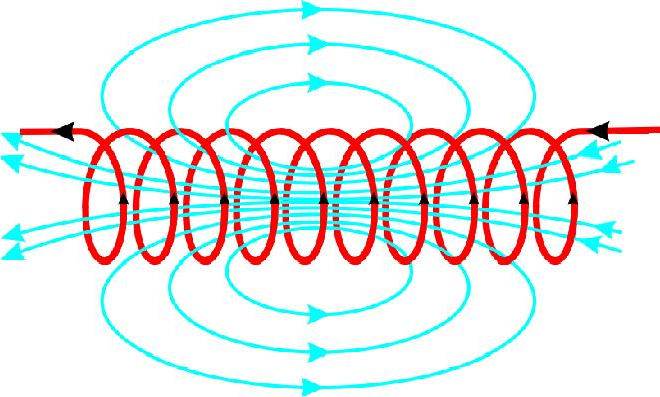
\includegraphics[height=3.8cm]{solenoid_field.png}};
  \node[anchor=north west,text width=9.4cm,font=\sffamily,align=left] at ([xshift=1.8cm,yshift=-10.8cm]current page.north west) {%
    {\large\bfseries Practise the way the exam asks.}\\[6pt]
    \small Every topic of the chapter, turned into questions you answer in this book:
    fill in the blanks, label and draw field lines, apply the hand rules, complete the
    derivation, solve the numerical, explain the reason. Each unit ends with a self check,
    and the book ends with a full 40-mark chapter test.\\[10pt]
    \faStar\ Marks badges: \badge{1M} \badge{2M} \badge{4M}\\[4pt]
    \faStar\ Academic standards: \asbadge{AS1} concept \asbadge{AS3} experiment \asbadge{AS5} diagram \asbadge{AS7} application\\[4pt]
    \faStar\ \tb\ marks every question from \emph{Improve your learning}};
  \node[anchor=south west,font=\sffamily] at ([xshift=1.8cm,yshift=2.2cm]current page.south west) {%
    \renewcommand{\arraystretch}{2.1}
    \begin{tabular}{@{}l@{\quad}p{8.5cm}@{}}
    \textbf{Name} & \hrulefill\\
    \textbf{Class / Section} & \hrulefill\\
    \textbf{Roll No.} & \hrulefill\\
    \textbf{School} & \hrulefill\\
    \end{tabular}};
\end{tikzpicture}
\null\clearpage

% =====================================================================
\section*{\sffamily\color{ecblue}How to use this workbook}
\begin{enumerate}[label=\textcolor{ecorange}{\faArrowRight},leftmargin=6mm]
\item Read the \textbf{Recall in 60 seconds} box first. If a point feels new, go back to the textbook page before you start.
\item Answer in the book, in pen. Do the questions \textbf{without} looking at the textbook, then check.
\item Numericals: \emph{formula $\rightarrow$ values in SI units (m, m$^2$, A, T) $\rightarrow$ answer with unit}.
\item Field-line diagrams: draw in pencil, put \textbf{arrows on every line}, mark N and S, $\odot$ and $\otimes$.
\item For every direction question, write which \textbf{rule} you used (thumb rule, right hand rule, Lenz's law).
\item Fill in the \textbf{Self check} after each unit; copy mistakes into the \textbf{Mistake log}.
\end{enumerate}

\subsection*{\sffamily\color{ecblue}What the exam asks from this chapter}
\renewcommand{\arraystretch}{1.35}
\begin{tabularx}{\linewidth}{>{\bfseries\sffamily}p{1.6cm}X}
\toprule
\rowcolor{ecblue}\textcolor{white}{Marks} & \textcolor{white}{\textbf{\sffamily Typical questions}}\\
\midrule
1 mark & Units (weber, tesla), one-line laws, energy change in motor/generator, force when parallel to $B$, MCQs.\\
2 marks & Direction of current/field/force from a figure, pole of a coil, TV distortion, closed field lines, short numericals on $B=\Phi/A$, $F=ILB$, $\varepsilon=Blv$, $\varepsilon=N\Delta\Phi/\Delta t$.\\
4 marks & Activities: current produces a field; force on a wire; Faraday's law. Working of motor and generators. Derivation of $\varepsilon=Blv$, $F=ILB$, $r=mv/Bq$. Lenz's law with energy argument. Levitation.\\
Diagrams & Field lines of bar magnet, straight wire, solenoid; right hand rules; coil in a field; motor; Faraday's activity; AC generator and emf graph.\\
\bottomrule
\end{tabularx}

\subsection*{\sffamily\color{ecblue}My progress tracker}
\renewcommand{\arraystretch}{1.55}
\begin{tabularx}{\linewidth}{>{\sffamily}l X c c c}
\toprule
\rowcolor{ecteal!15}\textbf{Unit} & \textbf{Topic} & \textbf{Score} & \textbf{Confidence} & \textbf{Revised on}\\
\midrule
1 & Oersted, magnetic field and field lines & \rule{1.3cm}{0.3pt} & \tick\,\tick\,\tick & \rule{1.6cm}{0.3pt}\\
2 & Magnetic flux and flux density & \rule{1.3cm}{0.3pt} & \tick\,\tick\,\tick & \rule{1.6cm}{0.3pt}\\
3 & Fields of a wire, coil and solenoid & \rule{1.3cm}{0.3pt} & \tick\,\tick\,\tick & \rule{1.6cm}{0.3pt}\\
4 & Force on a moving charge & \rule{1.3cm}{0.3pt} & \tick\,\tick\,\tick & \rule{1.6cm}{0.3pt}\\
5 & Force on a current; electric motor & \rule{1.3cm}{0.3pt} & \tick\,\tick\,\tick & \rule{1.6cm}{0.3pt}\\
6 & Induction: Faraday, Lenz, motional emf & \rule{1.3cm}{0.3pt} & \tick\,\tick\,\tick & \rule{1.6cm}{0.3pt}\\
7 & Applications, levitation, generators & \rule{1.3cm}{0.3pt} & \tick\,\tick\,\tick & \rule{1.6cm}{0.3pt}\\
-- & One-mark rapid fire & \rule{1.3cm}{0.3pt} & \tick\,\tick\,\tick & \rule{1.6cm}{0.3pt}\\
-- & Chapter test (40 marks) & \rule{1.3cm}{0.3pt} & \tick\,\tick\,\tick & \rule{1.6cm}{0.3pt}\\
\bottomrule
\end{tabularx}
{\small Confidence: tick one box for ``shaky'', two for ``fine'', three for ``I can teach it''.}

% =====================================================================
\unit{Magnetic field and field lines}{\badge{1M}\ \badge{2M}\ \badge{4M}}
% =====================================================================
\begin{recall}
\begin{itemize}[leftmargin=5mm,itemsep=0pt]
\item \key{Oersted (1820)}: a compass needle under a wire deflects when current flows $\Rightarrow$ a current produces a magnetic field.
\item A \key{magnetic field} is the region around a magnet where its force acts without contact. It has \textbf{strength} and \textbf{direction} and is three-dimensional.
\item \key{Field lines} are imaginary; the \textbf{tangent} gives the direction; crowded lines = strong field. Outside a magnet they go N $\to$ S. Uniform field: parallel, equally spaced lines.
\end{itemize}
\end{recall}

\exhead{A}{Fill in the blanks}{\asbadge{AS1}\ \badge{1M}}
\begin{enumerate}
\item The scientist who first showed that a current deflects a compass needle was \blank{Oersted}.
\item The direction of the field at a point is given by the \blank{tangent} to the field line at that point.
\item Field lines are \blank{crowded} near the poles, where the field is \blank{strong}.
\item A field whose strength and direction are the same everywhere is called a \blank{uniform} field.
\item Outside a bar magnet field lines go from \blank[1.5cm]{N} to \blank[1.5cm]{S}.
\end{enumerate}

\exhead{B}{True or false}{\asbadge{AS1}\ \badge{1M}}
{\small Write T or F. If false, correct it on the line below.}
\begin{enumerate}
\tf{Field lines of a magnet can cross each other.}{F}{They never cross; at a crossing the field would have two directions, which is impossible.}
\ifanswers\else\writelines{1}\fi
\tf{The magnetic field of a bar magnet exists only in the plane of the paper.}{F}{It is three-dimensional; it surrounds the magnet in all directions.}
\ifanswers\else\writelines{1}\fi
\tf{Far from a magnet a compass needle points almost north--south.}{T}{}
\ifanswers\else\writelines{1}\fi
\end{enumerate}

\exhead{C}{Label the Oersted apparatus}{\asbadge{AS5}\ \badge{2M}}
\begin{center}
\figlab{oersted_setup.png}{width=0.62\linewidth}{
\draw[fptr] (0.18,1.12) node[flab,anchor=south]{(a) \blank[2.3cm]{copper wire}} -- (0.36,0.82);
\draw[fptr] (0.85,1.12) node[flab,anchor=south]{(b) \blank[2.3cm]{battery}} -- (0.66,0.78);
\draw[fptr] (0.20,0.05) node[flab,anchor=north]{(c) \blank[2.3cm]{compass}} -- (0.40,0.60);
\draw[fptr] (0.72,0.05) node[flab,anchor=north]{(d) \blank[2.3cm]{key}} -- (0.54,0.40);}
\end{center}
\vspace{6pt}
\begin{enumerate}
\item What happens to the needle when the key is closed? What does it prove? \mk{2M}
\answer[3]{The needle deflects. When the key is opened it returns to the north--south direction. This proves that a current-carrying wire produces a magnetic field around it: electricity and magnetism are related.}
\end{enumerate}

\exhead{D}{Draw field lines}{\asbadge{AS5}\ \badge{2M}}
Draw at least six field lines of the bar magnet below, with arrows. \mk{2M}
\begin{center}
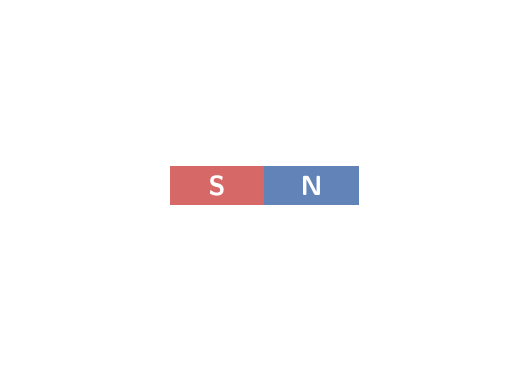
\begin{tikzpicture}
\fill[ecred!70] (-1.2,-0.25) rectangle (0,0.25); \fill[ecblue!70] (0,-0.25) rectangle (1.2,0.25);
\node[white,font=\sffamily\bfseries] at (-0.6,0) {S}; \node[white,font=\sffamily\bfseries] at (0.6,0) {N};
\ifanswers
\foreach \h in {0.8,1.4,2.1}{
  \draw[afl=0.5] (1.2,0.1) .. controls (2.5,\h) and (-2.5,\h) .. (-1.2,0.1);
  \draw[afl=0.5] (1.2,-0.1) .. controls (2.5,-\h) and (-2.5,-\h) .. (-1.2,-0.1);}
\draw[afl=0.5] (1.2,0) -- (3,0); \draw[afl=0.5] (-3,0) -- (-1.2,0);
\else
\draw[white] (-3,-2) rectangle (3,2);
\fi
\end{tikzpicture}
\end{center}

\exhead{E}{Short answers}{\tb\ \asbadge{AS1}\ \badge{2M}}
\begin{enumerate}
\item Are magnetic field lines closed? Explain. \mk{2M}
\answer[4]{Yes. Around a straight wire they are complete circles. For a solenoid (and a bar magnet) the lines outside go from N to S and continue inside from S to N, so every line is a closed loop.}
\item How can you find the strength and the direction of a magnetic field using field lines? \mk{2M}
\answer[3]{Direction: the tangent to the field line at the point (the way a compass needle points). Strength: how close the lines are; crowded lines mean a strong field, widely spaced lines a weak field.}
\end{enumerate}

\selfcheck{19}{
\item describe Oersted's experiment and its conclusion
\item state the properties of field lines
\item draw the field lines of a bar magnet with arrows}

% =====================================================================
\unit{Magnetic flux and flux density}{\badge{1M}\ \badge{2M}}
% =====================================================================
\begin{recall}
\begin{itemize}[leftmargin=5mm,itemsep=0pt]
\item \key{Magnetic flux} $\Phi$: number of field lines through a plane held perpendicular to the field. Unit \imp{weber (Wb)}.
\item \key{Flux density} $B=\dfrac{\Phi}{A}$ (area perpendicular to the field). Unit \imp{Wb/m$^2$ = tesla (T)}.
\item Plane tilted so its normal makes $\theta$ with $B$: effective area $A\cos\theta$, so \imp{$\Phi=BA\cos\theta$}. Plane parallel to $B$: $\Phi=0$.
\end{itemize}
\end{recall}

\exhead{A}{Fill in the blanks}{\asbadge{AS1}\ \badge{1M}}
\begin{enumerate}
\item The SI unit of magnetic flux is the \blank{weber}.
\item The SI unit of magnetic flux density is the \blank{tesla}, which equals \blank{Wb/m$^2$}.
\item Magnetic flux density is also called magnetic \blank{induction}.
\item The flux through a plane held parallel to the field is \blank[1.5cm]{zero}.
\end{enumerate}

\exhead{B}{Complete the derivation of $\Phi=BA\cos\theta$}{\asbadge{AS1}\ \badge{2M}}
\noindent
\begin{minipage}[c]{0.38\linewidth}\centering
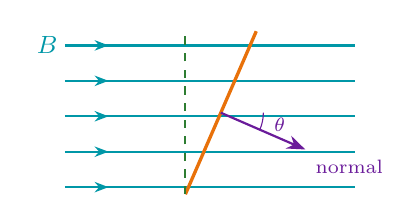
\begin{tikzpicture}[scale=0.9]
\foreach \y in {0.2,0.7,1.2,1.7,2.2} \draw[fl=0.15] (-0.5,\y) -- (3.6,\y);
\node[font=\small\bfseries,fieldc] at (-0.75,2.2) {$B$};
\draw[very thick,ecorange] (1.2,0.1) -- (2.2,2.4);
\coordinate (C) at (1.7,1.25);
\draw[-{Stealth},thick,ecpurple] (C) -- ($(C)+(-23.5:1.3)$) node[below right,font=\scriptsize]{normal};
\draw[ecpurple] ($(C)+(0.6,0)$) arc (0:-23.5:0.6); \node[font=\scriptsize,ecpurple] at ($(C)+(-12:0.85)$) {$\theta$};
\draw[thick,dashed,ecgreen] (1.2,0.1) -- (1.2,2.4);
\end{tikzpicture}\\{\small edge view of a plane of area $A$}
\end{minipage}\hfill
\begin{minipage}[c]{0.58\linewidth}
(1) $B$ uses the area \blank{perpendicular} to the field:\\ \hspace*{6mm}$B=\dfrac{\Phi}{A_\perp}$\\[4pt]
(2) The effective area perpendicular to the field is $A_\perp=\mblank{A\cos\theta}$.\\[4pt]
(3) So $B=\mblank[2.2cm]{\dfrac{\Phi}{A\cos\theta}}$ and $\Phi=\mblank[2.2cm]{BA\cos\theta}$.\\[4pt]
(4) $\theta=0^\circ$: $\Phi=\mblank{BA}$;\quad $\theta=90^\circ$: $\Phi=\mblank{0}$.
\end{minipage}

\exhead{C}{Numericals}{\asbadge{AS7}\ \badge{2M}}
\begin{worked}[Worked example: 0.02 Wb crosses 0.4 m$^2$ normally]
$B=\dfrac{\Phi}{A}=\dfrac{0.02}{0.4}=0.05$ T.\quad \textbf{Always} convert cm$^2$ to m$^2$ (1 cm$^2=10^{-4}$ m$^2$).
\end{worked}
\begin{enumerate}
\item $B=0.8$ T passes normally through a loop of area 0.05 m$^2$. Find the flux. \mk{2M}
\answer[2]{$\Phi=BA=0.8\times0.05=0.04$ Wb.}
\item The same loop is turned so that its normal makes $60^\circ$ with the field. Find the new flux. \mk{2M}
\answer[2]{$\Phi=BA\cos60^\circ=0.04\times\frac12=0.02$ Wb.}
\item A flux of $6\times10^{-4}$ Wb passes normally through 20 cm$^2$. Find $B$. \mk{2M}
\answer[3]{$A=20\times10^{-4}=2\times10^{-3}$ m$^2$. $B=\dfrac{6\times10^{-4}}{2\times10^{-3}}=0.3$ T.}
\end{enumerate}

\selfcheck{15}{
\item define magnetic flux and flux density with units
\item derive $\Phi=BA\cos\theta$ and use its special cases
\item convert areas to m$^2$ in numericals}

% =====================================================================
\unit{Fields of a wire, a coil and a solenoid}{\badge{1M}\ \badge{2M}\ \badge{4M}}
% =====================================================================
\begin{recall}
\begin{itemize}[leftmargin=5mm,itemsep=0pt]
\item \key{Straight wire}: field lines are concentric circles. \textbf{Right hand thumb rule}: thumb along current, curled fingers give the field. Out of the page $\odot$ $\Rightarrow$ anticlockwise; into the page $\otimes$ $\Rightarrow$ clockwise.
\item \key{Circular coil}: field at the centre is perpendicular to the plane of the coil. Curl fingers along the current, thumb gives $B$. Anticlockwise current (as seen) $\Rightarrow$ that face is \textbf{N}.
\item \key{Solenoid}: behaves like a bar magnet; outside N $\to$ S, inside S $\to$ N; lines are closed loops.
\end{itemize}
\end{recall}

\exhead{A}{Draw the field lines}{\asbadge{AS5}\ \badge{2M}}
Draw three field lines with arrows around each wire. \mk{2M}
\begin{center}
\begin{tabular}{c@{\hspace{2cm}}c}
\begin{tikzpicture}
\ifanswers\foreach \r in {0.5,0.9,1.3} \draw[anscol,thick,postaction={decorate},decoration={markings,mark=at position 0.25 with {\arrow{Stealth[length=5pt]}},mark=at position 0.75 with {\arrow{Stealth[length=5pt]}}}] (0,0) circle (\r);
\else\draw[white] (-1.4,-1.4) rectangle (1.4,1.4);\fi
\outpage{(0,0)}
\end{tikzpicture} &
\begin{tikzpicture}
\ifanswers\foreach \r in {0.5,0.9,1.3} \draw[anscol,thick,postaction={decorate},decoration={markings,mark=at position 0.25 with {\arrowreversed{Stealth[length=5pt]}},mark=at position 0.75 with {\arrowreversed{Stealth[length=5pt]}}}] (0,0) circle (\r);
\else\draw[white] (-1.4,-1.4) rectangle (1.4,1.4);\fi
\inpage{(0,0)}
\end{tikzpicture}\\
(1) current out of the page & (2) current into the page\\
\ifanswers{\small\color{anscol}anticlockwise}\fi & \ifanswers{\small\color{anscol}clockwise}\fi\\
\end{tabular}
\end{center}

\exhead{B}{Direction questions from the textbook}{\tb\ \asbadge{AS1}\ \badge{1M}\ \badge{2M}}
\noindent
\begin{minipage}[t]{0.22\linewidth}\centering
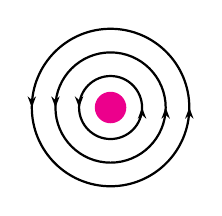
\begin{tikzpicture}[scale=0.5]
\foreach \r in {0.8,1.4,2.0} \draw[thick,postaction={decorate},decoration={markings,mark=at position 0.0 with {\arrow{Stealth[length=4pt]}},mark=at position 0.5 with {\arrow{Stealth[length=4pt]}}}] (0,0) circle (\r);
\fill[magenta] (0,0) circle (0.4);
\end{tikzpicture}\\{\small fig-Q1}
\end{minipage}\hfill
\begin{minipage}[t]{0.75\linewidth}
\begin{enumerate}
\item Field lines around a wire are shown in fig-Q1 (anticlockwise). What is the direction of the current? \mk{1M}
\answer[2]{Out of the page (towards the reader), by the right hand thumb rule.}
\end{enumerate}
\end{minipage}\\[6pt]
\begin{minipage}[t]{0.22\linewidth}\centering
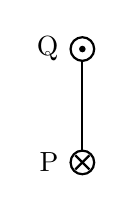
\begin{tikzpicture}[scale=0.6]
\draw[thick] (0,-1) -- (0,1);
\outpage[0.25]{(0,1.2)} \node[left] at (-0.3,1.2) {Q};
\inpage[0.25]{(0,-1.2)} \node[left] at (-0.3,-1.2) {P};
\end{tikzpicture}\\{\small fig-Q3}
\end{minipage}\hfill
\begin{minipage}[t]{0.75\linewidth}
\begin{enumerate}[start=2]
\item A coil is kept perpendicular to the page. At P the current flows into the page, at Q it comes out (fig-Q3). What is the direction of the field due to the coil? \mk{2M}
\answer[3]{At the centre, the wire at P (into page, clockwise field) gives a field to the right; the wire at Q (out of page, anticlockwise field) also gives a field to the right. So the field is along the axis of the coil, from left to right, perpendicular to the plane of the coil.}
\end{enumerate}
\end{minipage}\\[6pt]
\begin{minipage}[t]{0.22\linewidth}\centering
\begin{tikzpicture}[scale=0.55]
\draw[thick,postaction={decorate},decoration={markings,mark=at position 0.25 with {\arrow{Stealth[length=5pt]}},mark=at position 0.75 with {\arrow{Stealth[length=5pt]}}}] (0,0) circle (1);
\end{tikzpicture}\\{\small fig-Q4}
\end{minipage}\hfill
\begin{minipage}[t]{0.75\linewidth}
\begin{enumerate}[start=3]
\item The current in a coil flows as in fig-Q4 (anticlockwise as you see it). What pole is formed at this face? \mk{1M}
\answer[2]{North pole: curling the right-hand fingers anticlockwise, the thumb (field) points towards the viewer.}
\end{enumerate}
\end{minipage}

\exhead{C}{Label the solenoid}{\asbadge{AS5}\ \badge{2M}}
In the figure the current enters at the right end and leaves at the left. Mark the N and S ends and the direction of the field inside.
\begin{center}
\figlab{solenoid_field.png}{width=0.55\linewidth}{
\node[font=\sffamily\bfseries] at (-0.06,0.5) {\ifanswers\textcolor{anscol}{N}\else\fbox{\phantom{N}}\fi};
\node[font=\sffamily\bfseries] at (1.06,0.5) {\ifanswers\textcolor{anscol}{S}\else\fbox{\phantom{S}}\fi};
\ifanswers\draw[-{Stealth[length=6pt]},anscol,very thick] (0.75,0.5) -- (0.25,0.5) node[midway,below=6pt,font=\small]{inside: S $\to$ N};\fi}
\end{center}

\exhead{D}{Experiment}{\tb\ \asbadge{AS3}\ \badge{4M}}
Explain with the help of two activities that a current-carrying wire produces a magnetic field. \mk{4M}
\answer[12]{\textbf{Activity 1 (Oersted):} a wire stretched through the slits of two sticks is connected to a battery through a key; a compass is placed below it. When the key is closed the needle deflects; when it is opened the needle returns to N--S.\\
\textbf{Activity 4:} a vertical wire passes through a hole in a plank; 6--10 compass needles are placed on a circle around it. When the current flows, the needles set along tangents to the circle; iron filings sprinkled around form concentric circles.\\
\textbf{Conclusion:} the wire produces a magnetic field whose lines are concentric circles around it; the direction is given by the right hand thumb rule.}

\selfcheck{20}{
\item draw the field of a straight wire for both current directions
\item find the pole of a coil face from the current direction
\item describe the field of a solenoid and why its lines are closed loops}

% =====================================================================
\unit{Force on a moving charge}{\badge{1M}\ \badge{2M}\ \badge{4M}}
% =====================================================================
\begin{recall}
\begin{itemize}[leftmargin=5mm,itemsep=0pt]
\item A magnet distorts the picture on a CRT TV: the field exerts a force on the moving electrons.
\item \imp{$F=qvB\sin\theta$}; $F=qvB$ when $v\perp B$; $F=0$ when $v\parallel B$ or $v=0$.
\item Direction: right hand rule (forefinger $v$, middle finger $B$, thumb $F$), for a \textbf{positive} charge; reverse it for an electron. $F$ is always perpendicular to both $v$ and $B$.
\item A charge moving $\perp B$ goes round a circle: $r=\dfrac{mv}{Bq}$, $T=\dfrac{2\pi m}{Bq}$.
\end{itemize}
\end{recall}

\exhead{A}{Fill in the blanks}{\asbadge{AS1}\ \badge{1M}}
\begin{enumerate}
\item The force on a charge moving parallel to the field is \blank[1.5cm]{zero}.
\item The magnetic force is always perpendicular to both the \blank{velocity} and the \blank{field}.
\item For an electron, the direction of force is \blank{opposite} to that found for a positive charge.
\item The magnetic force on a charge moving $\perp B$ acts as the \blank{centripetal} force.
\end{enumerate}

\exhead{B}{Complete the derivation}{\asbadge{AS1}\ \badge{4M}}
A charge $q$ of mass $m$ moves with speed $v$ perpendicular to a uniform field $B$.\\[4pt]
(1) Magnetic force: $F=\mblank{qvB}$ \quad(since $\sin90^\circ=\mblank[1cm]{1}$).\\[4pt]
(2) This force is always perpendicular to the velocity, so the path is a \blank{circle}.\\[4pt]
(3) Centripetal force = magnetic force: \quad $\mblank{\dfrac{mv^2}{r}}=qvB$ \quad$\Rightarrow$\quad $r=\mblank[2cm]{\dfrac{mv}{Bq}}$\\[4pt]
(4) Time period $T=\dfrac{2\pi r}{v}=\mblank[2.2cm]{\dfrac{2\pi m}{Bq}}$, which does \blank{not} depend on the speed.

\exhead{C}{Numericals}{\asbadge{AS7}\ \badge{2M}}
\begin{enumerate}
\item A charge of $2\times10^{-6}$ C moves at $3\times10^4$ m/s perpendicular to $B=0.5$ T. Find the force. \mk{2M}
\answer[2]{$F=qvB=2\times10^{-6}\times3\times10^4\times0.5=3\times10^{-2}$ N.}
\item The same charge moves at $30^\circ$ to the field. Find the force. \mk{2M}
\answer[2]{$F=qvB\sin30^\circ=0.03\times\frac12=1.5\times10^{-2}$ N.}
\item A proton ($m=1.67\times10^{-27}$ kg, $q=1.6\times10^{-19}$ C) moves at $10^6$ m/s perpendicular to $B=1$ T. Find the radius of its path. \mk{2M}
\answer[3]{$r=\dfrac{mv}{Bq}=\dfrac{1.67\times10^{-27}\times10^6}{1\times1.6\times10^{-19}}=1.04\times10^{-2}$ m $\approx1$ cm.}
\end{enumerate}

\exhead{D}{Short answers}{\tb\ \asbadge{AS1}\ \badge{2M}}
\begin{enumerate}
\item Why does the picture appear distorted when a bar magnet is brought close to the screen of a television? \mk{2M}
\answer[3]{The picture on a CRT screen is made by a beam of fast-moving electrons. The magnet's field exerts a force $F=qvB\sin\theta$ on them, which changes their path, so they strike the wrong spots and the picture is distorted.}
\item State the right hand rule for the direction of force on a positive charge. \mk{2M}
\answer[3]{Stretch the thumb, forefinger and middle finger of the right hand mutually perpendicular. If the forefinger points along the velocity (or current) and the middle finger along the field, the thumb gives the direction of the force.}
\end{enumerate}

\selfcheck{25}{
\item use $F=qvB\sin\theta$ including the zero-force cases
\item find the direction of force with the right hand rule, and reverse it for electrons
\item derive $r=mv/Bq$ and $T=2\pi m/Bq$}

% =====================================================================
\unit{Force on a current; electric motor}{\badge{1M}\ \badge{2M}\ \badge{4M}}
% =====================================================================
\begin{recall}
\begin{itemize}[leftmargin=5mm,itemsep=0pt]
\item A current is moving charge, so a current-carrying wire in a field feels a force: \imp{$F=ILB\sin\theta$}; $F=ILB$ when $I\perp B$; $F=0$ when $I\parallel B$.
\item Activity 8: a wire in a horseshoe magnet is deflected; reversing the current or the poles reverses the deflection.
\item \key{Motor}: forces on opposite sides of a coil are equal and opposite (net force 0) but form a \textbf{couple} that rotates the coil. \textbf{Split rings} and brushes reverse the current every half turn. Electrical $\to$ mechanical energy.
\end{itemize}
\end{recall}

\exhead{A}{Complete the derivation of $F=ILB$}{\asbadge{AS1}\ \badge{4M}}
(1) Force on one charge moving with drift velocity $v$ perpendicular to $B$: $F_0=\mblank{qvB}$.\\[4pt]
(2) Total charge in the length $L$ inside the field is $Q$: $F=\mblank{QvB}$ \dots(1)\\[4pt]
(3) Time to cross length $L$: $t=\dfrac{L}{v}$, so $v=\mblank{\dfrac{L}{t}}$ \dots(2)\\[4pt]
(4) Put (2) in (1): $F=\mblank[2.2cm]{\dfrac{Q}{t}LB}$ \dots(3)\\[4pt]
(5) Since $\dfrac{Q}{t}=\mblank[1cm]{I}$, \quad $F=\mblank[1.6cm]{ILB}$. At an angle $\theta$: $F=\mblank[2cm]{ILB\sin\theta}$.

\exhead{B}{Numericals}{\tb\ \asbadge{AS7}\ \badge{2M}}
\begin{enumerate}
\item \tb\ An 8 N force acts on a 20 cm conductor placed perpendicular to a magnetic field. The current is 40 A. Find the magnetic field induction. \mk{2M}
\answer[3]{$L=0.2$ m. $B=\dfrac{F}{IL}=\dfrac{8}{40\times0.2}=1$ T.}
\item A wire 0.5 m long carries 4 A at $30^\circ$ to a field of 0.2 T. Find the force. \mk{2M}
\answer[2]{$F=ILB\sin30^\circ=4\times0.5\times0.2\times\frac12=0.2$ N.}
\end{enumerate}

\exhead{C}{Direction of force}{\tb\ \asbadge{AS1}\ \badge{2M}}
\noindent
\begin{minipage}[c]{0.3\linewidth}\centering
\begin{tikzpicture}[scale=0.6]
\foreach \x in {-2,...,2}{\foreach \y in {-1,...,1}{\node[font=\small] at (\x*0.6,\y*0.8) {$\times$};}}
\draw[line width=2pt] (0,-1.3) -- (0,1.6);
\draw[cur] (0.35,0.1) -- (0.35,1.3) node[right]{$i$};
\node at (-1.5,-1.4) {$B$};
\end{tikzpicture}\\{\small fig-Q5}
\end{minipage}\hfill
\begin{minipage}[c]{0.67\linewidth}
A straight wire carrying current $i$ upward is kept perpendicular to a field directed into the page; length $L$ is in the field. Find the magnitude and direction of the force. \mk{2M}
\answer[3]{Magnitude $F=iLB$ (since $\theta=90^\circ$). Right hand rule: forefinger up ($i$), middle finger into the page ($B$) $\Rightarrow$ thumb points to the \textbf{left}. The force acts to the left, in the plane of the page.}
\end{minipage}

\exhead{D}{Motor}{\asbadge{AS1}\ \asbadge{AS5}\ \badge{4M}}
\noindent
\begin{minipage}[c]{0.38\linewidth}\centering
\begin{tikzpicture}[scale=0.8]
\foreach \y in {-1.6,-0.8,0,0.8,1.6} \draw[fl=0.08] (-2.4,\y) -- (2.4,\y);
\node[font=\small\bfseries,fieldc] at (2.6,1.9) {$B$};
\draw[ecred,line width=2pt] (-1,-1.2) -- (-1,1.2) -- (1,1.2) -- (1,-1.2) -- cycle;
\draw[cur] (-1.25,-0.5) -- (-1.25,0.5); \draw[cur] (1.25,0.5) -- (1.25,-0.5);
\node[below left] at (-1,-1.2) {A}; \node[above left] at (-1,1.2) {B};
\node[above right] at (1,1.2) {C}; \node[below right] at (1,-1.2) {D};
\end{tikzpicture}
\end{minipage}\hfill
\begin{minipage}[c]{0.6\linewidth}
\begin{enumerate}
\item The force on AB is directed \blank{into the page} and on CD \blank{out of the page}.\mk{1M}
\item The net force on the coil is \blank[1.5cm]{zero}, yet the coil \blank{rotates} because the two forces form a \blank{couple}. \mk{1M}
\item Why is the current reversed every half turn, and which part does it? \mk{2M}
\answer[3]{After half a turn the forces would turn the coil back, so it would only rock to and fro. The split rings (commutator), rotating with the coil, swap brushes every half turn, reversing the current so the rotation continues in the same direction.}
\end{enumerate}
\end{minipage}

\exhead{E}{Experiment}{\tb\ \asbadge{AS3}\ \badge{4M}}
How do you verify experimentally that a current-carrying conductor experiences a force when kept in a magnetic field? \mk{4M}
\answer[10]{\textbf{Materials:} wooden plank, two split sticks, copper wire, 9 V battery, switch, horseshoe magnet.\\
\textbf{Procedure:} pass the wire through the splits of the sticks and connect it to the battery through the switch. Close the switch and bring the horseshoe magnet so the wire lies between its poles.\\
\textbf{Observation:} the wire is deflected (pushed up or down). Reversing the poles of the magnet, or the direction of the current, reverses the deflection.\\
\textbf{Conclusion:} a current-carrying conductor in a field experiences a force $F=ILB$; its direction is given by the right hand rule.}

\selfcheck{27}{
\item derive $F=ILB$ from $F=qvB$
\item find the direction of force on a wire with the right hand rule
\item explain the working of a motor, including split rings}

% =====================================================================
\unit{Induction: Faraday, Lenz and motional emf}{\badge{1M}\ \badge{2M}\ \badge{4M}}
% =====================================================================
\begin{recall}
\begin{itemize}[leftmargin=5mm,itemsep=0pt]
\item \key{Electromagnetic induction}: a current is induced in a coil when the flux through it changes (relative motion of magnet and coil).
\item \key{Faraday's law}: $\varepsilon=\dfrac{\Delta\Phi}{\Delta t}$; for $N$ turns $\varepsilon=N\dfrac{\Delta\Phi_0}{\Delta t}$.
\item \key{Lenz's law}: the induced current opposes the change in flux (conservation of energy). N pole approaching $\Rightarrow$ near face of coil becomes N.
\item \key{Motional emf}: $\varepsilon=Blv$ for a conductor of length $l$ moving with speed $v$ perpendicular to $B$.
\end{itemize}
\end{recall}

\exhead{A}{Activity 9: what does the galvanometer show?}{\asbadge{AS3}\ \badge{1M}}
\renewcommand{\arraystretch}{1.7}
\begin{tabularx}{\linewidth}{>{\small}X>{\small}X}
\toprule
\rowcolor{ecblue}\textcolor{white}{\textbf{Action}} & \textcolor{white}{\textbf{Galvanometer}}\\
\midrule
Magnet held at rest inside the coil & \blank{no deflection}\\
N pole pushed towards the coil & \blank{deflects one way}\\
N pole pulled away from the coil & \blank{deflects the opposite way}\\
S pole pushed towards the coil & \blank{deflects opposite to N pushed in}\\
Magnet pushed in faster & \blank{larger deflection}\\
\bottomrule
\end{tabularx}

\exhead{B}{Fill in the blanks}{\asbadge{AS1}\ \badge{1M}}
\begin{enumerate}
\item The current produced by changing flux is called the \blank{induced current}.
\item Lenz's law is a consequence of the conservation of \blank{energy}.
\item When the N pole of a magnet approaches a coil, the face of the coil nearer to it becomes a \blank[1.5cm]{north} pole.
\item $\varepsilon=Blv$ is called the \blank{motional emf}.
\end{enumerate}

\exhead{C}{Complete the derivation of $\varepsilon=Blv$}{\asbadge{AS1}\ \badge{4M}}
A cross wire of length $l$ lies on two parallel conductors in a uniform field $B$. It is moved a distance $s$ in time $\Delta t$ and a current $I$ flows.\\[4pt]
(1) Force of the field on the cross wire: $F=\mblank{BIl}$ \dots(8)\\[4pt]
(2) Work done by us in moving it: $W=Fs=\mblank{BIls}$ \dots(9)\\[4pt]
(3) Change in flux as the loop area changes by $ls$: $\Delta\Phi=\mblank{Bls}$ \dots(10) \;$\Rightarrow W=\mblank{I\,\Delta\Phi}$\\[4pt]
(4) Dividing by $\Delta t$: $P=\dfrac{W}{\Delta t}=\mblank{\dfrac{I\Delta\Phi}{\Delta t}}$; comparing with $P=\varepsilon I$ gives $\varepsilon=\mblank{\dfrac{\Delta\Phi}{\Delta t}}$\\[4pt]
(5) Also $P=Fv=\mblank{BIlv}$ (since $\dfrac{s}{\Delta t}=v$). So $\varepsilon I=BIlv$ \;$\Rightarrow\;\varepsilon=\mblank[1.6cm]{Blv}$

\exhead{D}{Numericals}{\tb\ \asbadge{AS7}\ \badge{2M}}
\begin{worked}[Worked example (textbook): 400 turns, flux per turn rises by 0.001 Wb in 0.1 s]
$\varepsilon=N\dfrac{\Delta\Phi_0}{\Delta t}=\dfrac{400\times0.001}{0.1}=4$ V. While the flux stays constant (0.1 s to 0.3 s), $\varepsilon=0$.
\end{worked}
\begin{enumerate}
\item \tb\ Find the length of a conductor moving at 10 m/s perpendicular to a field of 0.8 T if it induces an emf of 8 V. \mk{2M}
\answer[2]{$l=\dfrac{\varepsilon}{Bv}=\dfrac{8}{0.8\times10}=1$ m.}
\item The flux per turn in a coil of 100 turns falls from 0.05 Wb to 0.01 Wb in 0.2 s. Find the induced emf. \mk{2M}
\answer[3]{$\Delta\Phi_0=0.04$ Wb. $\varepsilon=\dfrac{100\times0.04}{0.2}=20$ V.}
\item A 1.5 m rod moves at 2 m/s perpendicular to $B=0.4$ T. Find the emf. \mk{2M}
\answer[2]{$\varepsilon=Blv=0.4\times1.5\times2=1.2$ V.}
\end{enumerate}

\exhead{E}{Figure questions}{\tb\ \asbadge{AS1}\ \asbadge{AS2}\ \badge{2M}}
\noindent
\begin{minipage}[c]{0.3\linewidth}\centering
\begin{tikzpicture}[scale=0.55]
\draw[magenta,thick] (0,0) ellipse (0.45 and 1.5);
\fill[gray!60] (1.4,-0.22) rectangle (4,0.22); \node[font=\small] at (1.7,0) {N};
\draw[-{Stealth}] (3.4,0.7) -- (1.8,0.7);
\end{tikzpicture}\\{\small fig-Q2}
\end{minipage}\hfill
\begin{minipage}[c]{0.67\linewidth}
\begin{enumerate}
\item A bar magnet with its N pole facing a coil moves towards it (fig-Q2). What happens to the flux through the coil? Which way does the induced current flow as seen from the magnet? \mk{2M}
\answer[3]{The flux through the coil increases. By Lenz's law the near face becomes N to repel the magnet, so the induced current is anticlockwise as seen from the magnet.}
\end{enumerate}
\end{minipage}\\[6pt]
\begin{minipage}[c]{0.3\linewidth}\centering
\begin{tikzpicture}[scale=0.55]
\fill[gray!60] (-3,-0.22) rectangle (-0.6,0.22); \node[font=\small] at (-0.9,0) {N};
\draw[-{Stealth}] (-2.4,0.7) -- (-0.8,0.7) node[right,font=\small]{$v$};
\draw[magenta,thick] (1,0) ellipse (0.45 and 1.5);
\draw[-{Stealth}] (0.6,1.9) -- (1.6,1.9) node[right,font=\small]{$v$};
\end{tikzpicture}\\{\small fig-Q6}
\end{minipage}\hfill
\begin{minipage}[c]{0.67\linewidth}
\begin{enumerate}[start=2]
\item \tb\ The coil and the bar magnet both move in the same direction with the same speed (fig-Q6). What happens? \mk{2M}
\answer[3]{There is no relative motion between the magnet and the coil, so the flux through the coil does not change. No emf is induced and no current flows.}
\end{enumerate}
\end{minipage}

\exhead{F}{Long answers}{\tb\ \asbadge{AS1}\ \asbadge{AS3}\ \badge{4M}}
\begin{enumerate}
\item Explain Faraday's law of induction with the help of an activity. \mk{4M}
\answer[10]{\textbf{Activity:} connect a coil to a galvanometer. Push the N pole of a bar magnet into the coil: the needle deflects. Hold it still: no deflection. Pull it out: the needle deflects the other way. With the S pole the deflections reverse. Moving the coil instead of the magnet gives the same result; faster motion gives a larger deflection.\\
\textbf{Law:} whenever the magnetic flux linked with a closed coil changes, an emf (and current) is induced. The induced emf equals the rate of change of flux: $\varepsilon=\dfrac{\Delta\Phi}{\Delta t}$; for $N$ turns, $\varepsilon=N\dfrac{\Delta\Phi_0}{\Delta t}$.}
\item State Lenz's law and show that it follows from the conservation of energy. \mk{4M}
\answer[9]{\textbf{Law:} the induced current flows in a direction that opposes the change in flux producing it.\\
\textbf{Energy argument:} push the N pole towards a coil. If the induced current made the near face S, it would attract the magnet, which would speed up by itself while electrical energy was also produced: energy from nothing, which is impossible. So the near face must be N and repel the magnet; we must do work to push it, and this work becomes electrical energy. Pulling the magnet away, the near face becomes S and attracts it, again opposing the motion.}
\item What experiment do you suggest to understand Faraday's law? What instruments are required? Give suggestions for good results and precautions. \mk{4M}
\answer[9]{\textbf{Experiment:} Activity 9 (magnet moved in and out of a coil connected to a galvanometer).\\
\textbf{Instruments:} coil of many turns of insulated copper wire, strong bar magnet, sensitive galvanometer, connecting wires.\\
\textbf{For good results:} use more turns, a stronger magnet and faster motion.\\
\textbf{Precautions:} tight connections; keep the galvanometer away from the magnet; check the zero before starting; move the magnet along the axis of the coil; do not drop the magnet.}
\end{enumerate}

\selfcheck{44}{
\item describe Activity 9 and state Faraday's law
\item state Lenz's law and give the energy argument
\item derive $\varepsilon=\Delta\Phi/\Delta t$ and $\varepsilon=Blv$
\item solve induced-emf numericals with $N$ turns}

% =====================================================================
\unit{Applications, levitation and generators}{\badge{1M}\ \badge{2M}\ \badge{4M}}
% =====================================================================
\begin{recall}
\begin{itemize}[leftmargin=5mm,itemsep=0pt]
\item Applications of induction: security metal detectors, tape recorder heads, induction stoves, ATM card readers.
\item \key{Levitation}: AC in a coil around an iron core $\Rightarrow$ changing flux through a metal ring $\Rightarrow$ induced current opposes it $\Rightarrow$ repulsion balances the ring's weight. With DC the ring only jumps at switch on/off.
\item \key{AC generator}: coil rotated in a field; full \textbf{slip rings}; emf zero when the coil is vertical, maximum when horizontal; reverses every half turn. \key{DC generator}: half (split) rings keep the output in one direction. Mechanical $\to$ electrical energy.
\end{itemize}
\end{recall}

\exhead{A}{Match the following}{\asbadge{AS1}\ \badge{1M}}
\renewcommand{\arraystretch}{1.3}
\begin{tabularx}{\linewidth}{@{}l l c X@{}}
\toprule
& \textbf{Column A} & & \textbf{Column B}\\
\midrule
1. & Induction stove & \bx{c} & a) Induced current in a large coil triggers an alarm\\
2. & Security check & \bx{a} & b) Magnetised tape moves past a small coil\\
3. & Tape recorder & \bx{b} & c) Induced current heats a metal pan\\
4. & Electric motor & \bx{e} & d) Mechanical energy into electrical energy\\
5. & Generator & \bx{d} & e) Electrical energy into mechanical energy\\
\bottomrule
\end{tabularx}

\exhead{B}{Levitation}{\asbadge{AS1}\ \asbadge{AS7}\ \badge{2M}\ \badge{4M}}
\begin{enumerate}
\item Why does the metal ring levitate when AC is used? \mk{4M}
\answer[8]{The ring is at rest, so the net force on it is zero: an upward force balances its weight. AC changes in size and direction continuously, so the flux through the ring keeps changing and a current is induced in it (Faraday). By Lenz's law this current opposes the change, so the ring's lower face always has the same polarity as the coil's upper face (e.g.\ coil top S, ring bottom S). The repulsion provides the upward force that holds the ring up.}
\item What happens if DC is used instead of AC? Why? \mk{2M}
\answer[3]{The ring jumps up only when the switch is closed (and again when it is opened) and then falls back, because the flux through the ring changes only at those instants. With a steady current there is no change of flux, no induced current and no repulsion.}
\end{enumerate}

\exhead{C}{AC generator}{\asbadge{AS1}\ \asbadge{AS5}\ \badge{2M}\ \badge{4M}}
\begin{enumerate}
\item Sketch the emf produced by an AC generator over one rotation, starting with the coil vertical. Mark where the emf is zero and maximum. \mk{2M}
\drawbox{4.5cm}{\begin{tikzpicture}
\begin{axis}[width=10cm,height=4cm,axis lines=middle,xmin=0,xmax=1.15,ymin=-1.3,ymax=1.3,
  xtick={0.25,0.5,0.75,1},xticklabels={$\frac14$,$\frac12$,$\frac34$,1},ytick=\empty,xlabel={rev.},ylabel={emf}]
\addplot[anscol,very thick,domain=0:1,samples=100] {sin(deg(2*pi*x))};
\node[font=\small,anscol] at (axis cs:0.25,1.15) {max (horizontal)};
\node[font=\small,anscol] at (axis cs:0.75,-1.15) {max reversed};
\end{axis}\end{tikzpicture}\\\small Zero at 0, $\frac12$, 1 rotation (coil vertical); maximum at $\frac14$ and $\frac34$ (coil horizontal).}
\item Why does the emf vary from zero to maximum during a rotation? \mk{2M}
\answer[3]{The emf depends on how fast the flux through the coil changes. When the coil is vertical (plane $\perp$ field) the flux is maximum but changing slowest, so the emf is zero. When it is horizontal (plane $\parallel$ field) the flux is changing fastest, so the emf is maximum.}
\item How is an AC generator converted into a DC generator? \mk{2M}
\answer[3]{Replace the two full slip rings by two half (split) rings. After every half rotation the ends of the coil change brushes, so the current in the external circuit always flows in the same direction (DC).}
\end{enumerate}

\exhead{D}{Textbook application}{\tb\ \asbadge{AS7}\ \badge{2M}}
Give a few applications of Faraday's law of induction in daily life. \mk{2M}
\answer[4]{Electric generators in power stations; metal detectors at security checks; tape recorder heads; induction stoves; ATM/credit card readers; transformers; bicycle dynamo.}

\selfcheck{25}{
\item explain four applications of induction
\item explain levitation with AC and why DC fails
\item explain the AC generator, its emf graph and the DC version}

% =====================================================================
\clearpage
\section*{\sffamily\color{ecblue}One-mark rapid fire}
{\small Answer in one word or one line. Target \textbf{8 minutes} for 25 questions.}\hfill Time taken: \rule{1.6cm}{0.3pt}\qquad Score: \rule{1cm}{0.3pt} / 25
\vspace{4pt}
\renewcommand{\arraystretch}{1.55}
\begin{multicols}{2}
\begin{enumerate}[itemsep=5pt]
\item Discovered the magnetic effect of current? \blank[2cm]{Oersted}
\item Unit of magnetic flux? \blank[2cm]{weber}
\item Unit of flux density? \blank[2cm]{tesla}
\item 1 T in N, A, m? \blank[2cm]{N/(A m)}
\item $\Phi$ for a plane $\parallel B$? \blank[2cm]{zero}
\item Field lines of a straight wire? \blank[2cm]{circles}
\item Current $\odot$: field lines are? \blank[2cm]{anticlockwise}
\item Rule for field of a wire? \blank[2cm]{thumb rule}
\item Anticlockwise current face is? \blank[2cm]{N pole}
\item Coil that acts like a bar magnet? \blank[2cm]{solenoid}
\item Force on a charge moving $\parallel B$? \blank[2cm]{zero}
\item Formula for force on a charge? \blank[2cm]{$qvB\sin\theta$}
\item Radius of path of a charge? \blank[2cm]{$mv/Bq$}
\item Force on a current $\perp B$? \blank[2cm]{$ILB$}
\item Motor converts? \blank[2cm]{elec.\ $\to$ mech.}
\item Reverses current in a motor? \blank[2cm]{split rings}
\item Faraday's law formula? \blank[2cm]{$\Delta\Phi/\Delta t$}
\item Law giving induced current direction? \blank[2cm]{Lenz's law}
\item Lenz's law is based on? \blank[2cm]{energy cons.}
\item Motional emf? \blank[2cm]{$Blv$}
\item Emf when coil plane $\perp B$ (generator)? \blank[2cm]{zero}
\item Rings in an AC generator? \blank[2cm]{slip rings}
\item Generator converts? \blank[2cm]{mech.\ $\to$ elec.}
\item Stove using induction? \blank[2cm]{induction stove}
\item Current reversing periodically? \blank[2cm]{AC}
\end{enumerate}
\end{multicols}

% =====================================================================
\clearpage
\section*{\sffamily\color{ecblue}Score boosters}
\subsection*{\sffamily Anatomy of a full-marks 4-mark answer}
{\small Example question: \emph{Explain the working of an electric motor.}}\par\vspace{2pt}
\renewcommand{\arraystretch}{1.5}
\begin{tabularx}{\linewidth}{>{\bfseries\sffamily\small}p{2.6cm}X>{\small}p{2.7cm}}
\toprule
\rowcolor{ecteal!15}Part & \textbf{What to write} & \textbf{Why it matters}\\
\midrule
1. Principle & A current-carrying coil in a field experiences a force ($F=ILB$). & Scores the concept mark.\\
2. Diagram & Coil ABCD between N and S, split rings, brushes, battery; arrows for current. & Diagrams carry marks.\\
3. Forces & AB and CD: equal, opposite forces $\Rightarrow$ couple $\Rightarrow$ rotation. & Shows you know why.\\
4. Commutator & Split rings reverse current every half turn $\Rightarrow$ continuous rotation. & Key idea examiners look for.\\
5. Energy & Electrical energy $\to$ mechanical energy. & Closes the answer.\\
\bottomrule
\end{tabularx}

\subsection*{\sffamily Keywords the examiner looks for}
\renewcommand{\arraystretch}{1.35}
\begin{tabularx}{\linewidth}{>{\bfseries\small}p{3.8cm}>{\small}X}
\toprule
Oersted & compass deflects $\cdot$ current produces field\\
Field lines & tangent gives direction $\cdot$ crowded = strong $\cdot$ closed loops\\
Straight wire & concentric circles $\cdot$ right hand thumb rule\\
Force & $qvB\sin\theta$ $\cdot$ $ILB\sin\theta$ $\cdot$ zero when parallel $\cdot$ right hand rule\\
Motor & couple $\cdot$ split rings $\cdot$ brushes $\cdot$ electrical to mechanical\\
Faraday & change of flux $\cdot$ rate of change $\cdot$ induced emf\\
Lenz & opposes the change $\cdot$ conservation of energy\\
Generator & rotating coil $\cdot$ slip rings $\cdot$ zero/maximum emf $\cdot$ mechanical to electrical\\
\bottomrule
\end{tabularx}

\begin{examtip}[Mistakes that cost marks]
\begin{multicols}{2}\small
\begin{itemize}[leftmargin=4mm,itemsep=1pt]
\item Field lines without arrows.
\item $\theta$ measured from the plane, not the normal, in $\Phi=BA\cos\theta$.
\item Forgetting $F=0$ when parallel to $B$.
\item Not reversing the force for an electron.
\item Using cm or cm$^2$ without converting.
\item Forgetting $N$ in $\varepsilon=N\Delta\Phi_0/\Delta t$.
\item Slip rings in a motor (it has split rings).
\item No energy argument in Lenz's law.
\end{itemize}
\end{multicols}
\end{examtip}

\subsection*{\sffamily Formula sheet \normalfont\small(cover the right column and test yourself)}
\renewcommand{\arraystretch}{1.7}
\begin{tabularx}{\linewidth}{>{\bfseries\small}p{5.3cm}X}
\toprule
\rowcolor{ecred}\textcolor{white}{Quantity} & \textcolor{white}{\textbf{Formula / unit}}\\
\midrule
Flux density & $B=\dfrac{\Phi}{A}$ \quad tesla = Wb/m$^2$\\
Flux & $\Phi=BA\cos\theta$ \quad weber\\
Force on a charge & $F=qvB\sin\theta$\\
Circular motion & $r=\dfrac{mv}{Bq}$,\quad $T=\dfrac{2\pi m}{Bq}$\\
Force on a current & $F=ILB\sin\theta$\\
Faraday's law & $\varepsilon=\dfrac{\Delta\Phi}{\Delta t}$;\quad $\varepsilon=N\dfrac{\Delta\Phi_0}{\Delta t}$\\
Motional emf & $\varepsilon=Blv$\\
\bottomrule
\end{tabularx}

\subsection*{\sffamily Diagram practice tracker}
{\small Draw each diagram three times on separate days. Tick when you can draw it from memory in under 4 minutes.}\par
\renewcommand{\arraystretch}{1.4}
\begin{tabularx}{\linewidth}{X c c c}
\toprule
\textbf{Diagram} & \textbf{Try 1} & \textbf{Try 2} & \textbf{Try 3}\\
\midrule
Field lines of a bar magnet & \tick & \tick & \tick\\
Field of a straight wire ($\odot$ and $\otimes$) & \tick & \tick & \tick\\
Field of a solenoid with N and S & \tick & \tick & \tick\\
Right hand rule for force & \tick & \tick & \tick\\
Electric motor with split rings & \tick & \tick & \tick\\
Faraday's activity (magnet, coil, galvanometer) & \tick & \tick & \tick\\
AC generator and emf graph & \tick & \tick & \tick\\
\bottomrule
\end{tabularx}

% =====================================================================
\clearpage
\section*{\sffamily\color{ecblue}Chapter test}
\begin{tcolorbox}[wbox,colback=ecblue!5,colframe=ecblue]
\sffamily\small\textbf{Time: 1 hour 30 minutes \hfill Maximum marks: 40}\\[2pt]
\rmfamily Section I: 6 questions $\times$ 1 mark. Section II: 5 questions $\times$ 2 marks. Section III: 4 questions $\times$ 4 marks, each with an internal choice. Section IV: 8 multiple choice questions $\times$ 1 mark.
\end{tcolorbox}

\exhead{Section I}{}{\badge{6 $\times$ 1 = 6}}
\begin{enumerate}
\item What is the SI unit of magnetic flux density? \answer[1]{Tesla (Wb/m$^2$).}
\item State Lenz's law. \answer[1]{The induced current opposes the change in flux producing it.}
\item What is the force on a current-carrying wire kept parallel to a magnetic field? \answer[1]{Zero.}
\item Which device converts mechanical energy into electrical energy? \answer[1]{Generator.}
\item Write the formula for motional emf. \answer[1]{$\varepsilon=Blv$.}
\item Name the rule used to find the direction of the field around a straight wire. \answer[1]{Right hand thumb rule.}
\end{enumerate}

\exhead{Section II}{}{\badge{5 $\times$ 2 = 10}}
\begin{enumerate}[resume]
\item Why does a TV picture get distorted when a magnet is brought near it? \answer[3]{The picture is made by moving electrons; the magnet's field exerts a force on them and deflects them.}
\item A 0.5 m wire carries 2 A perpendicular to a field of 0.4 T. Find the force. \answer[2]{$F=ILB=2\times0.5\times0.4=0.4$ N.}
\item A coil of 50 turns has its flux per turn changed by 0.02 Wb in 0.1 s. Find the induced emf. \answer[2]{$\varepsilon=\frac{50\times0.02}{0.1}=10$ V.}
\item Are magnetic field lines closed? Explain. \answer[3]{Yes: circles round a wire; for a solenoid/magnet the lines go N $\to$ S outside and S $\to$ N inside.}
\item A coil and a magnet move together in the same direction at the same speed. Is a current induced? Why? \answer[3]{No: no relative motion, so no change of flux.}
\end{enumerate}

\exhead{Section III}{}{\badge{4 $\times$ 4 = 16}}
\begin{enumerate}[resume]
\item Explain with two activities that a current-carrying wire produces a magnetic field.\\
\textbf{OR}\quad Describe an activity to show that a current-carrying wire experiences a force in a magnetic field.
\answer[8]{See Unit 3, Exercise D or Unit 5, Exercise E.}
\item Derive $F=ILB$ for a straight wire in a magnetic field.\\
\textbf{OR}\quad Derive $r=\dfrac{mv}{Bq}$ and $T=\dfrac{2\pi m}{Bq}$ for a charge moving perpendicular to a field.
\answer[8]{See Unit 5, Exercise A or Unit 4, Exercise B.}
\item Derive $\varepsilon=Blv$ using conservation of energy.\\
\textbf{OR}\quad State Faraday's law and explain it with an activity.
\answer[8]{See Unit 6, Exercise C or Exercise F1.}
\item Explain the working of an electric motor with a diagram.\\
\textbf{OR}\quad Explain the working of an AC generator with the graph of emf for one rotation.
\answer[8]{See the anatomy table in Score boosters (motor) or Unit 7, Exercise C.}
\end{enumerate}

\exhead{Section IV}{}{\badge{8 $\times$ 1 = 8}}
\begin{enumerate}[resume]
\mcq{Which converts electrical energy into mechanical energy?}{motor}{battery}{generator}{switch}{A}
\mcq{The force on a wire perpendicular to a uniform field is}{0}{$ILB$}{$2ILB$}{$ILB/2$}{B}
\mcq{One tesla is equal to}{N/C}{N/(A m)}{A/m}{N/(A s)}{B}
\mcq{Unit of magnetic flux is}{dyne}{oersted}{gauss}{weber}{D}
\mcq{No force acts on a current-carrying conductor kept}{parallel to the field}{perpendicular to the field}{in the field}{away from the field}{A}
\mcq{Current flows anticlockwise in a coil as you see it. The face towards you is}{S pole}{N pole}{neither}{both}{B}
\mcq{In an AC generator the emf is maximum when the plane of the coil is}{perpendicular to $B$}{parallel to $B$}{at $45^\circ$}{at rest}{B}
\mcq{The time period of a charge moving in a circle in a uniform field depends on}{its speed}{the radius}{$m$, $q$ and $B$}{none}{C}
\end{enumerate}

\vspace{6pt}
\begin{tcolorbox}[wbox,colback=ecgold!10,colframe=ecorange,title={\faChartLine\ My test result}]
\renewcommand{\arraystretch}{1.6}
\begin{tabularx}{\linewidth}{X c c c c c}
Section & I & II & III & IV & \textbf{Total}\\
Marks & \rule{0.9cm}{0.3pt}\,/6 & \rule{0.9cm}{0.3pt}\,/10 & \rule{0.9cm}{0.3pt}\,/16 & \rule{0.9cm}{0.3pt}\,/8 & \rule{0.9cm}{0.3pt}\,/40\\
\end{tabularx}
\end{tcolorbox}

% =====================================================================
\clearpage
\section*{\sffamily\color{ecblue}Mistake log}
{\small Write every question you got wrong. Redo it after one week without looking at the answer.}\par\vspace{4pt}
\renewcommand{\arraystretch}{2.5}
\begin{tabularx}{\linewidth}{|p{1.4cm}|X|X|c|}
\hline
\rowcolor{ecblue!12}\textbf{Unit / Q} & \textbf{What I wrote} & \textbf{The correct idea} & \textbf{Redone}\\\hline
\logrow\logrow\logrow\logrow\logrow\logrow\logrow\logrow\logrow\logrow\logrow\logrow\logrow\logrow
\end{tabularx}

\end{document}
